%%%%% Single page layout:
%%%%% ----------------------------------------------------
\documentclass[12pt, a4paper]{report}
\setlength\textwidth{160mm}
\setlength\textheight{247mm}
\setlength\oddsidemargin{0mm}
\setlength\evensidemargin{0mm}
\setlength\topmargin{0mm}
\setlength\headsep{0mm}
\setlength\headheight{0mm}
\let\openright=\clearpage
\usepackage[utf8]{inputenc}

%%% Additional useful packages
%%% ----------------------------------------------------------------
\usepackage{array}
\usepackage{amsmath}  
\usepackage{amssymb}
\usepackage{amsfonts}       
\usepackage{amsthm}      
\usepackage{algorithm2e}
\usepackage{algorithmic}
\usepackage{bm}
\usepackage[mathscr]{euscript}
\usepackage{graphicx}       
\usepackage{psfrag}         
\usepackage{fancyvrb}    
\usepackage{float}
\usepackage[square,sort,comma,numbers]{natbib}        
\usepackage{bbding}         
\usepackage{dcolumn}        
\usepackage{booktabs} 
\usepackage{multirow}
\usepackage{paralist}       
\usepackage{indentfirst}    
\usepackage[nottoc,notlof,notlot]{tocbibind}
\usepackage{url}
\usepackage{tabularx}
\usepackage{subcaption}
\usepackage[unicode]{hyperref}
\hypersetup{pdftitle=LiDAR obstacle detection and avoidance, 
            pdfauthor=Alojz Gomola,
            colorlinks=false,
            urlcolor=blue,
            pdfstartview=FitH,
            pdfpagemode=UseOutlines,
            pdfnewwindow,
            breaklinks
          }
\usepackage{array}
\newcolumntype{L}[1]{>{\raggedright\let\newline\\\arraybackslash\hspace{0pt}}m{#1}}
\newcolumntype{C}[1]{>{\centering\let\newline\\\arraybackslash\hspace{0pt}}m{#1}}
\newcolumntype{R}[1]{>{\raggedleft\let\newline\\\arraybackslash\hspace{0pt}}m{#1}}         

\newcommand{\FIGDIR}{./Pics}    %%% directory containing figures
\newcommand{\twolinecellr}[2][r]{%
  \begin{tabular}[#1]{@{}r@{}}#2\end{tabular}}
\theoremstyle{plain}
\newtheorem{theorem}{Theorem}
\newtheorem{lemma}[theorem]{Lemma}
\newtheorem{proposition}[theorem]{Proposition}

\theoremstyle{plain}
\newtheorem{definition}{Definition}
\newtheorem{problem}{Problem}
\newtheorem{example}{Example}
\newtheorem{assumption}{Assumption}

\theoremstyle{remark}
\newtheorem*{corollary}{Corollary}
\newtheorem*{note}{Note}



\newenvironment{dokaz}{
  \par\medskip\noindent
  \textit{Proof}.
}{
\newline
\rightline{\SquareCastShadowBottomRight}
}


%\bibliographystyle{plainnat}     %% Author (year) style
\bibliographystyle{unsrt}        %% [number] style
\setcitestyle{square}


\title{FEUP research plan}
\author{Alojz Gomola}
\date{May 2016}

%%%%% ------------------------------------------------------------
\DefineVerbatimEnvironment{PCinout}{Verbatim}{fontsize=\small, frame=single}



\newcommand{\R}{\mathbb{R}}
\newcommand{\N}{\mathbb{N}}

\DeclareMathOperator{\pr}{\textsf{P}}
\DeclareMathOperator{\E}{\textsf{E}\,}
\DeclareMathOperator{\var}{\textrm{var}}
\DeclareMathOperator{\sd}{\textrm{sd}}


\newcommand{\T}[1]{#1^\top}        

\newcommand{\goto}{\rightarrow}
\newcommand{\gotop}{\stackrel{P}{\longrightarrow}}
\newcommand{\maon}[1]{o(n^{#1})}
\newcommand{\abs}[1]{\left|{#1}\right|}
\newcommand{\dint}{\int_0^\tau\!\!\int_0^\tau}
\newcommand{\isqr}[1]{\frac{1}{\sqrt{#1}}}
\newcommand{\norm}[1]{\left\lVert#1\right\rVert}


\newcommand{\pulrad}[1]{\raisebox{1.5ex}[0pt]{#1}}
\newcommand{\mc}[1]{\multicolumn{1}{c}{#1}}

\begin{document}

%Title page 
\pagestyle{empty}
\begin{center}

%header
{FACULDADE DE ENGENHARIA DA UNIVERSIDADE DO PORTO}

\vspace{3cm}
{\LARGE\bfseries Optimal Control of Unmanned Air Vehicles with Obstacle Avoidance Capabilities in
Partially Known Environment}\\
\vspace{1cm}
{\LARGE Exam report}

\vspace{1cm}
{\LARGE Alojz Gomola}


\vspace{5cm}
\centerline{\mbox{
\includegraphics[width=60mm]{\FIGDIR/feuplogo.eps}}}


\vspace{2cm}
{\LARGE Doutoramento em Matemática Aplicada}

\vspace{1.5cm}
\begin{tabular}{rl}  
\noalign{\vspace{2mm}}
Supervisors: & Dr. Fernando Manuel Ferreira Lobo Pereira\\
\noalign{\vspace{2mm}}
& Dr. João Tasso de Figueiredo Borges de Sousa\\ 
\end{tabular}

\vspace{2cm}
{January 31,2017}
\end{center}

\newpage
\openright

\pagestyle{plain}
\setcounter{page}{1}

\tableofcontents


%%% List of figures
\newpage
\listoffigures

%%% List of tables
\newpage
\listoftables
\chapter*{Nomenclature}
\noindent
This chapter describe used symbols (\ref{tab:symbols}), acronyms (\ref{tab:acronym}) and organizations (\ref{tab:organizations}) mentioned in work. It is recommended to review this chapter before reading work.
\begin{table}[H]
    \centering
    \begin{tabularx}{\textwidth}{|l||X|}
    \hline
    Acronym & Meaning\\ \hline\hline
    UAV & Unmanned Aerial Vehicle\\ \hline
    UAS & Unmanned Autonomous System(including naval vehicles)\\ \hline
    RPAS & Remotely Piloted Aerial System(lesser degree of autonomy)\\ \hline
    LOS & Line Of Sight\\ \hline
    VLOS & Visual Line Of Sight\\ \hline
    BLOS & Behind Line Of Sight\\ \hline
    SAA & Sense And Avoid\\ \hline
    DAA & Detect And Avoid \\ \hline
    CD\&R & Collision Detection and Resolution\\ \hline
    RTK & Real-Time Kinematik\\ \hline
    GPS & Global Positioning System\\ \hline
    IMU & Internal Measurement Unit\\ \hline
    LiDAR &  Light Detection and Ranging \\ \hline
    ADS-B & Automatic Dependent Surveillance – Broadcast\\ \hline
    LTI & Linear Time Invariant\\ \hline
    LTV & Linear Time Varying\\ \hline
    NTI & Non-linear Time Invariant\\ \hline
    NTV & Non-linear Time Varying\\ \hline
    \end{tabularx}
    \caption{List of Acronyms}
    \label{tab:acronym}
\end{table}

\begin{table}[H]
    \centering
    \begin{tabularx}{\textwidth}{|l||X|}
    \hline
    Acronym & Organization name \\ \hline\hline
    EASA & European Aviation Safety Agency \\ \hline 
    JARUS&  Joint Authorities for Regulation of Unmanned Systems\\ \hline
    LSTS & Laboratório de Sistemas e Tecnologia Subaquática\\ \hline
    FEUP &Faculdade de Engenharia da Universidade do Porto\\ \hline
    ITK & Institutt for teknisk kybernetikk NTNU\\ \hline
    NTNU& Norges teknisk-naturvitenskapelige universitet\\ \hline
    IST & Instituto Superior Técnico - Universidade de Lisboa\\ \hline
    HWI & Honeywell international\\ \hline
    \end{tabularx} 
    \caption{List of Organizations}
    \label{tab:organizations}
\end{table}

\begin{table}[H]
    \centering
    \begin{tabularx}{\textwidth}{|l||X|}
    \hline
    Symbol & Explanation \\ \hline\hline
    $A,B,C,D,\dots$ & Capital letters are used for matrixes\\\hline
    $A(\dots),B(\dots),\dots$ & Functional matrixes, $(\dots)$ denotes parameters\\\hline
    $f(\dots),g(\dots),\dots$ & Vector or scalar functions $(\dots)$ denotes parameters\\\hline
    $\vec{f}(\dots),\vec{g}(\dots),\dots$ & Implicit vector functions, when equation contains both types of scalar and vector functions.\\\hline
    $t,x,y,z,\dots$ & Vector or scalar coeficients \\\hline
    $\vec{x},\vec{o},\vec{g},\dots$ & Implicit vectors, when function containst both vec types of scalar and vector coeficients.\\\hline
    $\theta,\varphi$ & Greek letters denoting angles in radians\\\hline
    $\mathscr{O}$ & Set of known obstacles $o_i\in\mathscr{O}$ where each obstacle $o_i$ is parametrized.\\\hline
    $\mathscr{D}$ & Threat set of obstacles endangering vehicle\\\hline
    $\mathscr{R},R$ & Reach set (Invariant if not stated other), defines safe space where vehicle can move without intermediate or future crash.\\\hline
    $\mathscr{F}$ & Partially known space, space examined by vehicle during flight.\\\hline
    $\mathscr{O},\bar{\mathscr{O}}$ & Obstacle space, space occupied by obstacle.\\\hline
    $\mathscr{U},\bar{\mathscr{U}}$& Uncertain space, space hidden behind obstacle or unexplored space.\\\hline
    $\omega$ & Control input function, defining current control input of system\\\hline
    $\Omega$ & Control strategy, set of continuous control input functions $\omega_i\in\Omega$ which does not lead vehicle to crash in known space $\mathscr{F}$\\\hline
    $\gamma$ & Voting algorithm, deciding most feasible control input $\omega_i$ from control strategy $\Omega$\\\hline
    \textnormal{atan2} & $\arctan$ function normalizing angle around adjacent line in interval $(-\pi,\pi]$\\ \hline 

    \end{tabularx} 
    \caption{List of symbols}
    \label{tab:symbols}
\end{table}
\chapter{Introduction}\label{ch:introduction}

\section{Objectives of the report}\noindent
This work concerns the use of dynamic optimization - optimal control and calculus of variations - techniques to address the problem of optimally controlling an Unmanned Aircraft Vehicle (UAV) in an uncertain environment. Special emphasis will be placed in avoiding collision with obstacles.

Modern day avoidance systems are based on rule system implementation \cite{benjamin2006navigation}. Rule systems are technical bridge between law and implementation. These rules are putting additional high level constraints to optimal control problem.  Rich constraint programming languages have been developed for expressing and combining constraints and specifying search procedures at a high level of abstraction. Local search approaches to combinatorial optimization are able to deliver optimal control to vehicles \cite{hentenryck2009constraint}. The first of approaches delivered in constrained search are given \cite{grefenstette1986optimization}. All mentioned approaches revolves around keeping optimum principle in high level control in partially known environment. Methods varies from logical programming applications to performance based search. Software engineering methods for abstract path searching can be response for optimal path problem \cite{korf1985depth}.

Solution to given abstract problem consist of interdisciplinary usage of various method:
\begin{enumerate}
    \item\textit{Rule engine application} - rules impact decision making of overall system, this part of control system is viewed as event based control.
    \item\textit{Path switching} - events given by rules can impact path switching, previously optimal path may not be viable, therefore new optimal path needs to be derived in near real-time conditions. Decision making can be viewed as part of artificial intelligence field. 
    \item\textit{Higher level optimality principle} - higher level of control mechanism is used to abstract from controlled plant and enables fast optimal path calculation
    \item\textit{Lower level optimality principle}- standard low level control mechanism guarantying optimal execution of higher level control commands.
\end{enumerate}

\newpage
\section{Motivation}\noindent
Problem of obstacle avoidance can be applied to any type if vehicle \textit{ground, aerial or marine}. Obstacle avoidance can be separated into two categories. \textit{Three dimensional avoidance} for aerial and subsurface marine vehicles  and \textit{Two dimensional avoidance} for ground and surface marine vehicles. This work focus on \textit{Three dimensional avoidance} with partially known boundaries. Results of this work can be applied to both categories of \textit{subsurface marine} and \textit{aerial} vehicles. The only difference is that in \textit{subsurface marine} obstacle avoidance boundary of water surface exists. Boundary of \textit{water floor} and \textit{ground bed} are similar, despite fact that vehicles dynamics is different. Example of marine vehicle obstacle avoidance can be found in \cite{benjamin2006navigation}. Example of vehicle avoidance equipment can be found in \cite{chey1986vehicle}. There exists representations where Sonar and LiDAR Inputs are exchangeable \cite{fiorini1998motion}. 
\noindent
Optimal path planning in partially known environment is critical for following reasons:
\begin{enumerate}
    \item \textit{Safety guarantee} - guarantee safety of vehicle and prevent it destruction.
    \item \textit{Energy consumption} - prolong vehicle operational capabilities to maximal extent.
\end{enumerate}
Main motivation is  \textit{energy consumption aspect}. Path planning for UAV with focus on low energy consumption is given by \cite{bortoff2000path}. Some of the works are taking inspiration form  nature, like \cite{ma2007improved}. Other was specialized on predictive control in urban environment \cite{singh2001trajectory}. Proposition for optimal control problem to optimal parameter problem is given by \cite{hull1997conversion}. This proposition is key enabler for conversion of optimal control problem in continuous time to discrete parameter problem. 
\noindent
The problem of many optimal control approaches mentioned beforehead is that they are using optimum principle in continuous time. This work focus on The proposed approach combines abstract sensing technology with techniques based on controlled invariance in discrete time. Sensors fusion provides a abstract representation of the world in the field of view of the sensors. Controlled invariance techniques provide a characterization of flight envelopes that by design avoid obstacles under reasonable assumptions. 
\begin{figure}[H]
    \centering
    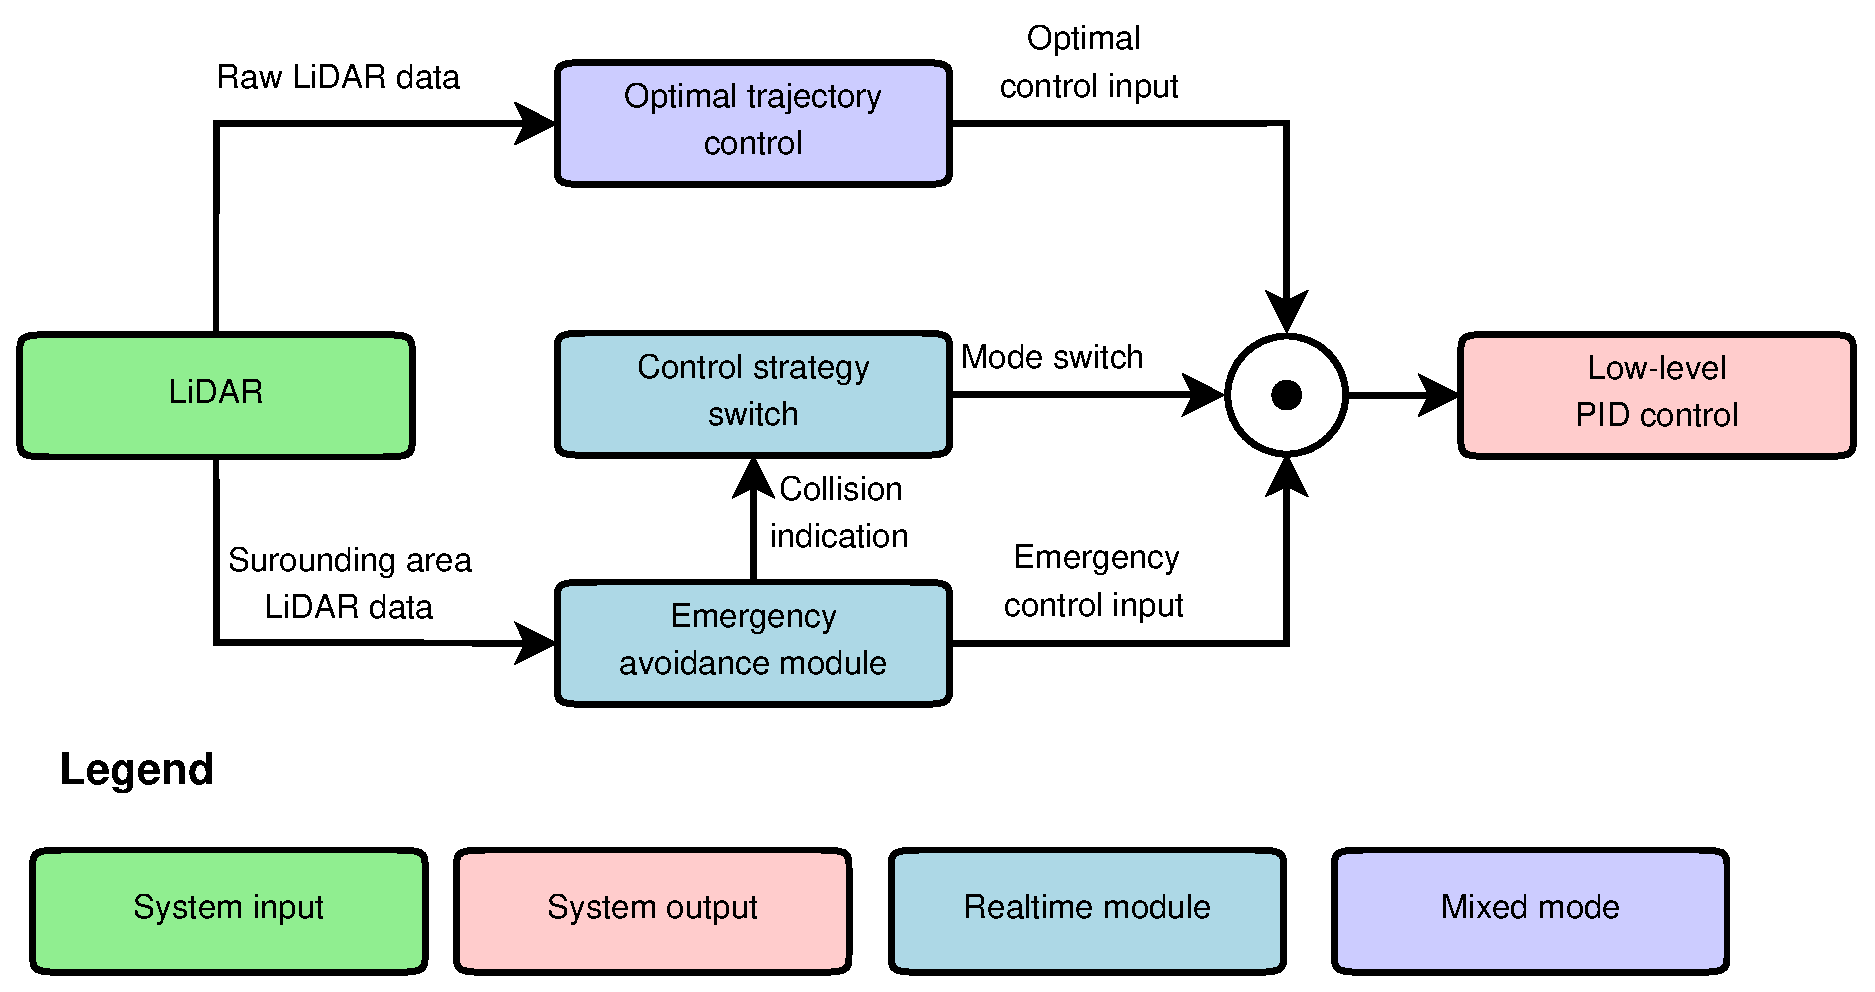
\includegraphics[width=10cm]{Pics/35_ControlConcept.eps}
    \caption{Control concept scheme}
    \label{fig:ControlConcept}
\end{figure}
\noindent
The approach presents a nested solution to control design depicted in Figure \ref{fig:ControlConcept}. There is a nominal trajectory for the UAV that may be generated by an  \textit{Optimal trajectory control} module. Sensor will continuously scan the environment for obstacles. If an obstacle crosses a pre-computed safety zone then an \textit{Emergency avoidance module} is invoked to override the trajectory tracking controller. \textit{Emergency avoidance module} is invoked and keeps vehicle at semi-optimal avoidance path, with premise that vehicle will return to original planned path. The safety zone is computed using invariance techniques based on reach set computations. When the obstacle no longer presents a threat (i.e., it does not belong to the safety zone) control is returned to \textit{Optimal trajectory control} module. This nested control approach entails  a \textit{Control strategy switch} will override control input of system and starts avoidance maneuver to achieve \textit{reactive avoidance}.
%\textit{UAV} is usually used for two types of missions, or rather \textit{operation types}:
%\begin{enumerate}
%    \item \textit{Delivery} - deliver usable point from point A to point B.
%    \item \textit{Surveillance} - fly trough defined area. 
%\end{enumerate}
%It is expected that UAV returns from mission unharmed. 
%\section{Approach}



\section{Goals}\noindent
Main goals of this work is to provide following artefacts, which will contribute to complex obstacle avoidance system:
\begin{enumerate}
    \item\textit{Optimal control translation from higher to lower level} - translation of high level commands to lower level continious signal. This is one of main goal of the thesis
    \item\textit{Control architecture for optimal control} - provide control framework architecture combining event based, discrete time higher level optimal control and continuous lower level optimal control.
    \item\textit{Decision frame for high level decisions} - outline decision frame for event based system in control switch (fig. \ref{fig:ControlConcept}).
\end{enumerate}
%\noindent
%The goal of the research is to develop an integrated approach to real-time obstacle detection and avoidance for Unmanned Air Vehicles (UAV) based on %\textit{LiDAR} technology. The approach concerns the solution of the following sub-problems:
%\begin{enumerate}
%    \item \textit{Obstacle detection and sensor fusion} - processing \textit{LiDAR} data into an unified and compact data representation for obstacle detection. 
%		
%    \item \textit{Real-time reactive obstacle avoidance} - identify safety problems and perform avoidance maneuvers with safety guarantees when collisions are possible and return control to nominal controller when collision is avoided.
%\end{enumerate}

\section{Organization of the report}\noindent
Report is organized in following manner:
\begin{itemize}
    \item\textit{Chapter \ref{ch:introduction}.} presents motivation, goals and objectives of report.
    \item\textit{Chapter \ref{ch:UAVControlProblem}.} defines control principle with emphasis to principle of optimality. It also outlines assumptions used for proof of concept.
    \item\textit{Chapter \ref{ch:stateofArt}.} provides overview of reach sets, movement automaton and other theoretical supplements used in this work.
    \item\textit{Chapter \ref{ch:problemFormulation3D}} provides problem formulation and it is addressing issues of optimal control.
    \item\textit{Chapter \ref{ch:controlapproach3D}} describes control approach in detail with used techniques with emphasis on optimal control.
    \item\textit{Chapter \ref{ch:controlapproach3D}.} revolves around control approach on higher level framework and movement automaton $\mathscr{MA}$ movements $\mathscr{m_i(t_i)}$ translation to continious signal.
    \item\textit{Chapter \ref{ch:simulationResults}.} is focused on simulation results of proposed optimal control approach, it outlines preliminaries of obstacle avoidance framework.
\end{itemize}


 






\chapter{The UAV control problem}\label{ch:UAVControlProblem}
\noindent This chapter specifies optimal control architecture for UAV and defines assumptions.
\section{The control problem}
\noindent \textit{Obstacle avoidance} in terms of control is complex optimisation problem with dynamic constraints. Movement constraints are mainly given by static uncharted obstacles and non-cooperative intruders. This work focus on uncharted obstacles. Non-cooperative intruders are omitted in this work. Usually multiple layer control concept is used. Control concept used for this work is in fig. \ref{fig:controlConceptIntro}.
\begin{figure}[H]
    \centering
    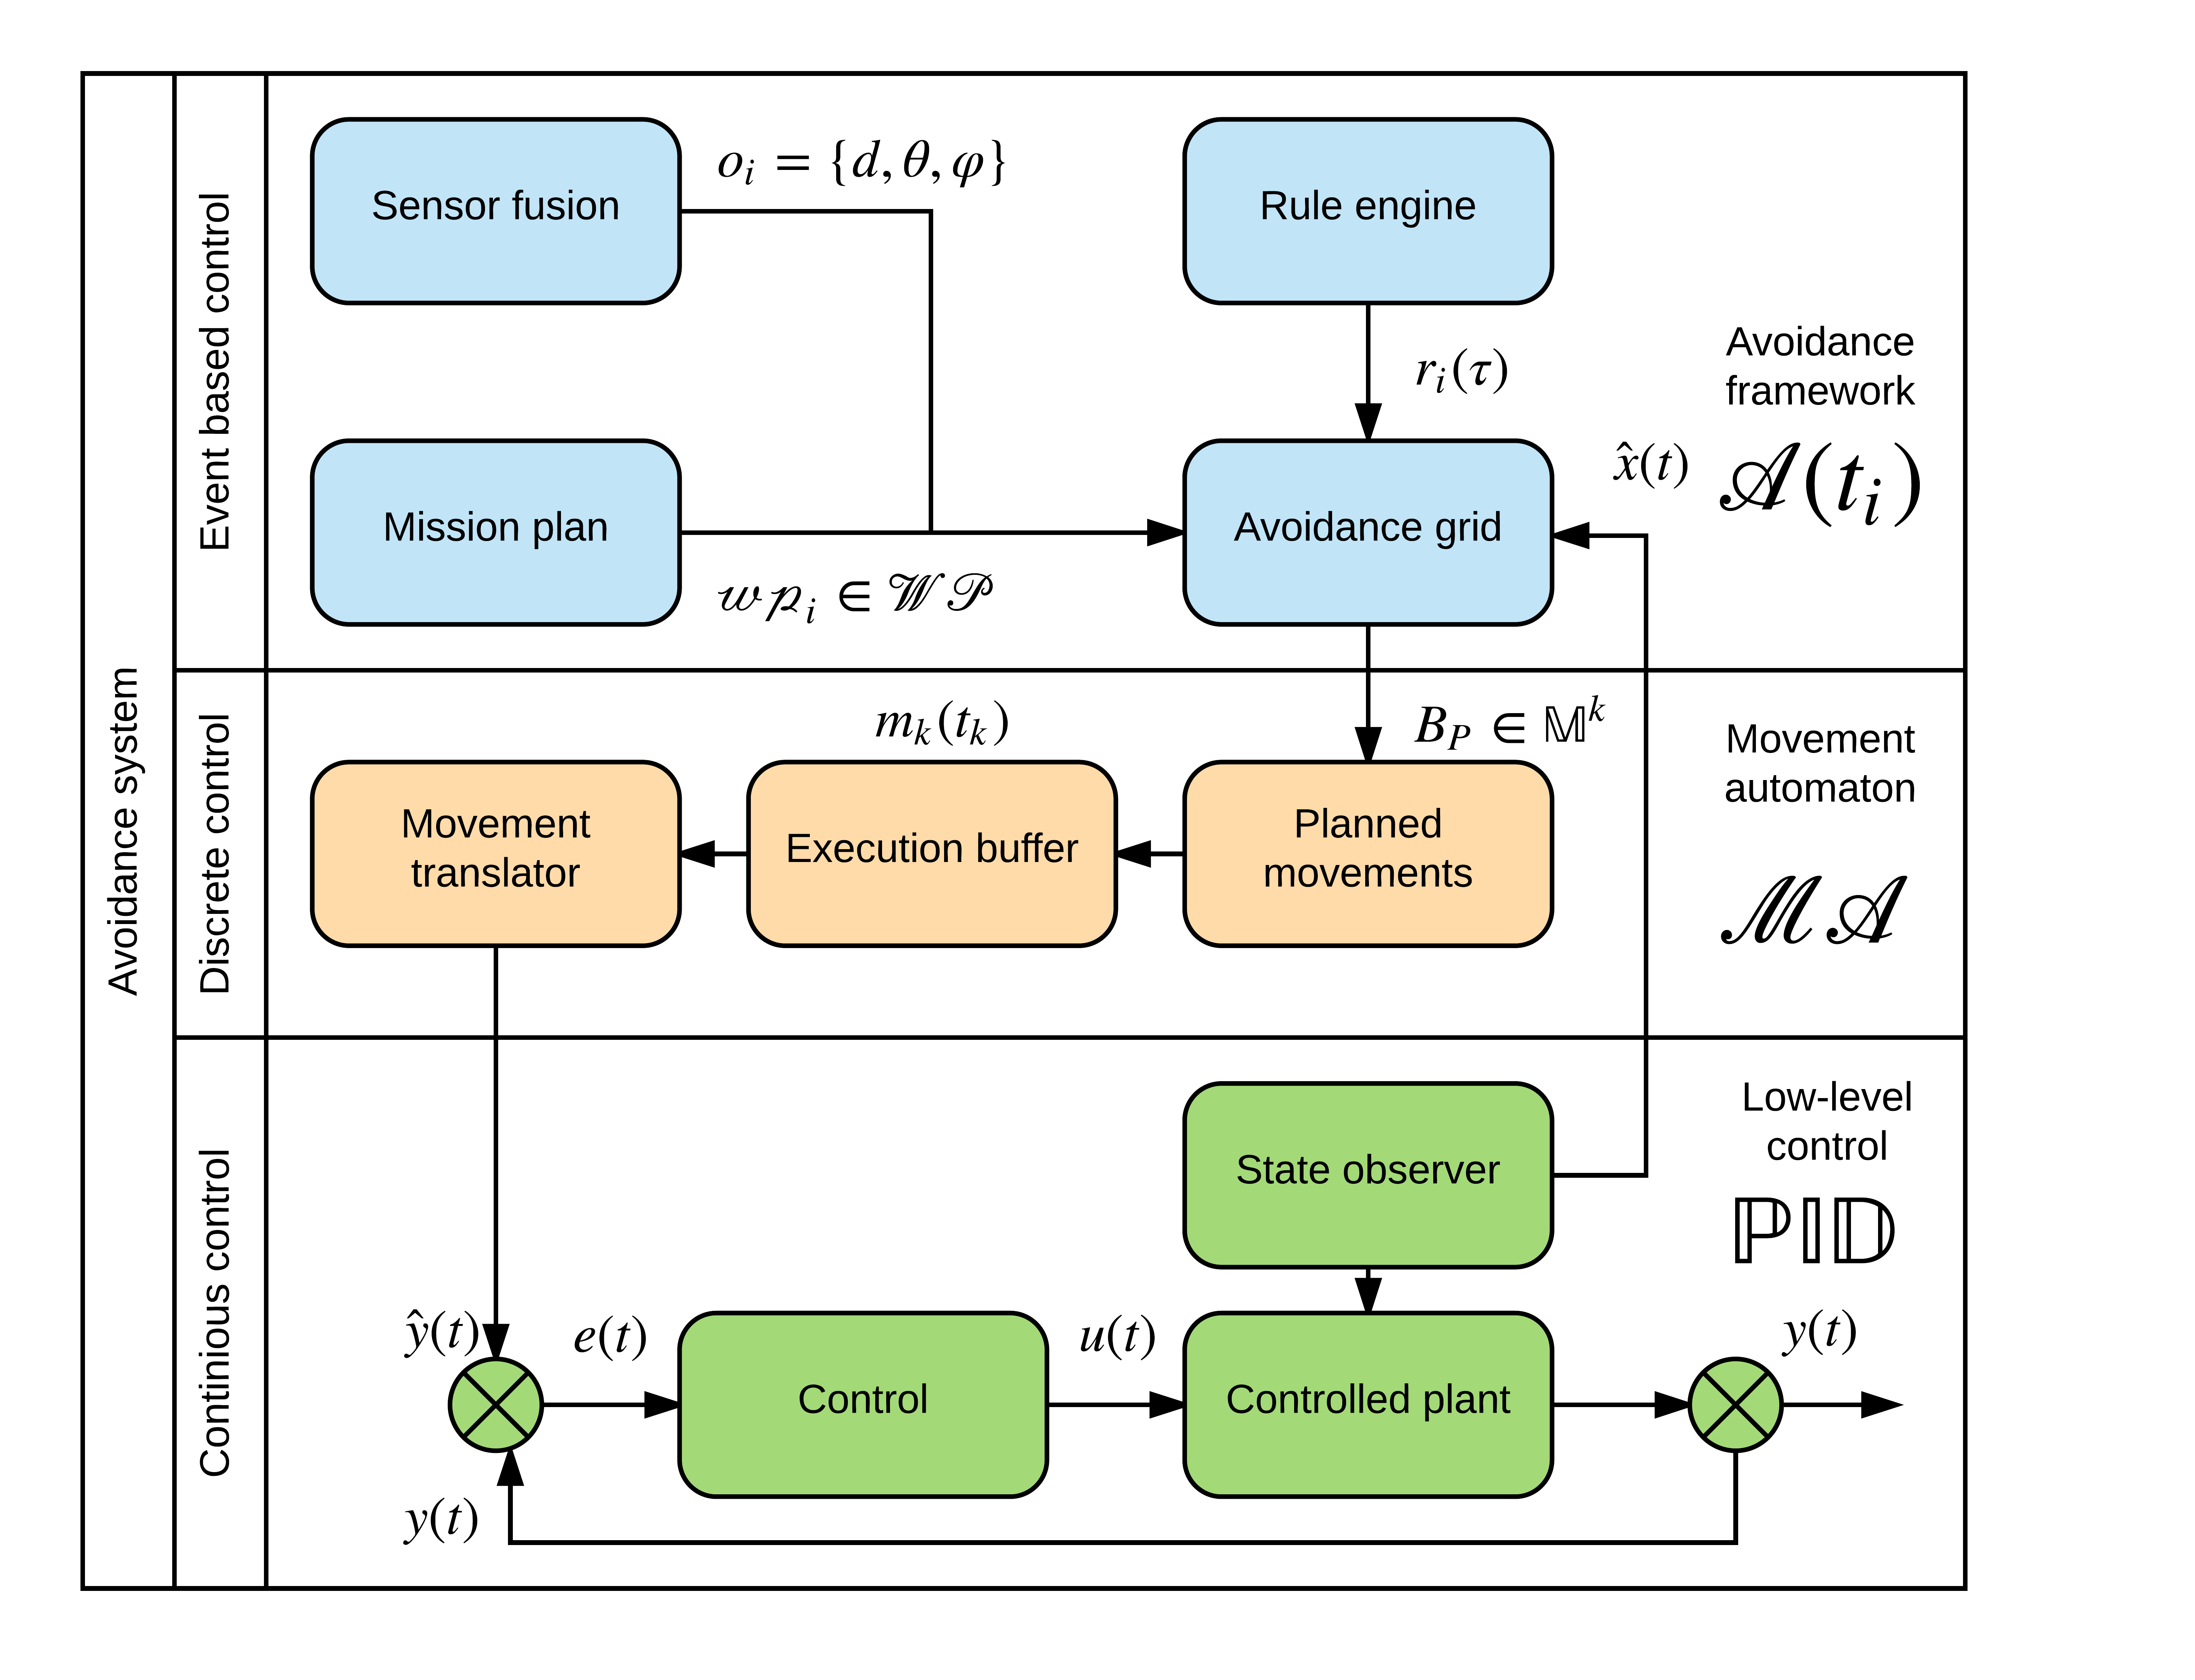
\includegraphics[width=.95\linewidth]{\FIGDIR/72_Control_Concept.png}
    \caption{Decision frame $\mathscr{D}(0)$.}
    \label{fig:controlConceptIntro}
\end{figure}

\noindent \textit{Event based control} module is responsible for high level decisions and mission execution. This module generates high level input commands which are optimal to given criterion. \textit{Event based control} consist from following artifacts:
\begin{enumerate}
    \item \textit{Sensor fusion} - fuses data from sensor system with observed system state $\hat{x}$, outputs detected obstacles $o_i\in\mathscr{O}$.
    \item \textit{Mission plan} - contains mission plan $\mathscr{WP}$, determines navigation goal waypoint $\mathscr{WP}_g$.
    \item \textit{Rule engine} - determines additional constraints for avoidance grid $\mathscr{A}(t_i)$, determines escape goal in avoidance grid $c_{i,j,k}$.
    \item \textit{Avoidance grid} - responsible for optimal path planning in partially known space, consumes observed system state $\hat{x}(t)$, rule engine decisions $r_i(\tau)$, obstacle set $o_i\in\mathscr{O}$ and goal waypoint $\mathscr{WP}_i$, produces avoidance command chain $B_p \in \mathbb{M}^k$.
\end{enumerate}

\noindent \textit{Discrete control} module is responsible for processing high level movement command chain $B_p \in \mathbb{M}^k$. It is implemented as special type of open hybrid automaton, movement automaton $\mathscr{MA}$. Movement automaton $\mathscr{MA}$ have following notable artifacts:
\begin{enumerate}
    \item \textit{Planned movements} - buffers planned movements from avoidance grid $B_P\in\mathbb{M}^k$, planed movements buffer can be extended by additional movements (normal situation) or filled with new movement chain(flush) in case of trajectory correction or avoidance. Planned movement is similar to FIFO stack.
    \item \textit{Execution buffer} - executes first command from \textit{planned movements}, based on previous movement $m_{k-1}(t_{(k-1)})$ and actual command $m_k(t_k)$ chain of movement primitives $\{p_1, \dots p_l\}$ is created. Chain of movement primitives $\{p_1, \dots p_l\}$ is forwarded to movement translator.
    \item \textit{Movement translator} - translates chain of movement primitives or other movement representation to:
    \begin{enumerate}[a.]
        \item \textit{Desired input signal $\hat{u}(t),t\in<t_{(k-1)},t_k)$,} - in case of \textit{open loop control}, in this case desired control signal is feed directly to \textit{controlled plant}.
        \item \textit{Desired output signal $\hat{y}(t),t\in<t_{(k-1)},t_k)$} - in case of \textit{closed loop control}, in this case desired output signal is feed to closed loop controller. If there is closed loop controller, there is possibility for low level optimisation of control.
    \end{enumerate}
\end{enumerate}

\noindent \textit{Continuous control} module is target for low level control optimisation techniques. It is expected that \textit{controlled plant} is observable at least at position and orientation state parameters. \textit{State observer} provides observed state within critical time frame. \textit{Continuous control} module is responsible for low level control of plant with following artifacts:
\begin{enumerate}
    \item \textit{Control} - standard closed loop control component, using error $e(t)$ as input and actuating unit signal $u(t)$ as output.
    \item \textit{Controlled plant} - controlled vehicle plant, can be subsurface marinal vehicle or aerial vehicle
    \item \textit{State observer} - observing state of controlled plant $\hat{x}(t)$.
\end{enumerate}

\subsection*{Trajectory optimization technique}
\noindent \textit{Trajectory} is constrained by set of waypoints $\mathscr{WP}$ and set of obstacles $\mathscr{O}$. Obstacle set $\mathscr{O}$ is constantly evolving, based on sensor system reading and area of interest (offline obstacle map). \textit{Trajectory search} in constantly changing environment is problem which needs to address following concurrent requirements:
\begin{enumerate}
    \item \textit{Calculation time} - avoidance trajectory calculation time must be shortest possible to assure optimal \textit{prediction window}.
    \item \textit{Estimation precision} - avoidance trajectory estimation must be precise enough to guarantee safety of predicted trajectory. Predicted trajectory with some estimation error, should not lead to vehicle crash. 
    \item \textit{Estimation optimality} - predicted trajectory should minimize optimality criterion or cost function $J(\circ)$.
\end{enumerate}
\noindent Discrete time optimisation techniques are used on obstacle avoidance framework $\mathscr{A}(t_i)$ in \textit{event based control} module.  Continuous optimisation techniques to increase movement automaton $\mathscr{MA}$ execution precision can be used in \textit{closed loop control}. Chosen optimisation techniques for movement chain optimisation is \textit{rapid exploration tree}. This optimisation technique is not trivial search technique and it demonstrates qualities of discrete time optimum search.

\subsection*{Type of sensory data and its processing}
\noindent \textit{LiDAR is main sensor}. There is planned addition for \textit{ADS-B} transceiver/receiver for moving cooperative obstacle SAA. LiDAR data are represented as positional vector $\vec{p}=[d,\theta,\varphi]$, where $d$ is distance to point, $\theta$ is horizontal offset angle and $\varphi$ is vertical offset angle in local coordinates frame. Only one matter point $\vec{p}$ is scanned at given scanning time $t_s$, in case of LiDAR sensor with one active scanner. 

LiDAR data for one LiDAR sweep at time interval $(t_s, t_e] $are given as series of points and scanning time pairs $\left\{\{\vec{p}_1\,t_s\},\{\vec{p}_2,t_2\},\dots,\{\vec{p}_n,t_e\}\right\}$. These points needs to be normalized at time $t_e$ in \textit{local coordinate frame} with center at vehicle position $[x_v,y_v,z_v]$ and rotated by vehicle orientation $[-\alpha_v,-\beta_v,-\gamma_v]$. One LiDAR sweep covers area given by scanning distance $[d_s,d_e]$, horizontal range $[\theta_s,\theta_e]$ and vertical range $[\varphi_s,\varphi_e]$. One LiDAR sweep covers rectangular conical cut in front of the scanning vehicle.

For global coordinates Earth geocentric reference model \textit{WGS-84} is used, therefore \textit{GPS} is considered as main source of position. In later stages mixed position mode using \textit{GLONASS} system can be incorporated. \textit{GLONASS} is using \textit{PG-90} reference model. Transformation between \textit{PG-90} and \textit{WGS-84} are mentioned in \cite{misra1996integrated}. For further mentions of \textit{global coordinate frame} reference frame \textit{WGS-84} is always used.

\textit{Obstacle map} is using global coordinate frame, where obstacles are represented by center of their mass $\vec{p}_c$ and protective range $r$. Obstacle body is then given by unit ball around $\mathscr{B}(\vec{p}_c,r)$.

\newpage\noindent\textit{Sensor fusion} is fusing following data sources in local coordinate frame of vehicle:
\begin{enumerate}
    \item \textit{LiDAR sensor sweep (approximated)} - based on LiDAR sensor reading point-cloud in front of vehicle is filtered by EKF \cite{blanc2005ekf}. Visibility space is then partitioned into \textit{free, obstacle} and \textit{uncertain} subspaces.
    \item \textit{Obstacle map (planned)} - based on known obstacle map, the obstacles in FOV range are selected and fused into vehicle`s local coordinate frame. Free space previously unoccupied by by obstacles is marked as \textit{map obstacle occupied}.
    \item \textit{Intruders (planned)} - based on ADS-B reading and LiDAR data processing moving cooperative and non-cooperative intruders are identified. Portions of free space occupied by intruders in expected reach time are then marked as \textit{intruder occupied}.
\end{enumerate}

\noindent Result of \textit{sensor fusion} is then used as base of \textit{avoidance frame} $\mathscr{A}(t_i)$ at time of avoidance $t_i$.

\subsection*{Obstacle avoidance}
\noindent \textit{Obstacle avoidance} is continuous process which is triggered by collision detection system. When \textit{Control strategy switch} changes mode to obstacle avoidance following steps are executed until return to optimal trajectory:
\begin{enumerate}
    \item \textit{Space assessment} - main contributor is sensor fusion giving space status in local coordinate frame. FOV is segmented into \textit{free} and \textit{occupied} space. 
    \item \textit{Reachable space determination} - decides which portions of \textit{free} space are accessible by vehicle control. Reach set $\mathscr{R}$ numeric or analytical approximation plays key role in this step.
    \item \textit{Goal of avoidance determination} - based on chain of rules $r(\tau)$ from \textit{Rule engine} module,current goal waypoint $\mathscr{WP}_g$ from \textit{Mission plan} module and reachable space $\mathscr{R}$ in \textit{Avoidance grid} module $\mathscr{A}(t_i)$ goal of avoidance $c_g$ is determined in FOV. 
    \item \textit{Avoidance trajectory determination} - based on determined avoidance goal and space constrained by $\mathscr{R}$ optimal movement chain $\left\{m_1(t_1),\dots,m_i(t_i)\right\}$ is generated. This process is main focus of this work and semi-optimality of movement planning, using movement automaton $\mathscr{MA}$ as main control input. Generated movement chain is optimal in FOV.
\end{enumerate}

\noindent Avoidance trajectory $\mathscr{T}(\vec{x}_i,t_i)$ generated for state $\vec{x}_i$ at decision time $t_i$. Executed movement buffer is given by chained avoidance frames $\mathscr{A}$ at decision times $t_{d_1},\dots,t_{d_n}$. Final chained trajectory $\mathscr{T}= \cup_{i=\{d_1,\dots,d_n\}} \mathscr{T}(\vec{x}_{i},t_i)$ is semi-optimal in known world and optimal in partially known world, due uncertainty \cite{kochenderfer2008encounter}.

\newpage\subsection*{Control switch strategy}
\noindent If planned trajectory is going to enter into \textit{uncertain}, \textit{obstacle} or \textit{occupied} space in FOV processed by \textit{Sensor fusion}. Then avoidance frame $\mathscr{A}(t_i)$ is created. Avoidance frame $\mathscr{A}(t_i)$ can be invoked by execution of rule $r_i(\tau)$ at time $\tau$ from \textit{Rule engine} module. In both cases \textit{Control strategy switch} (fig. \ref{fig:ControlConcept}). is triggered. 

\textit{Vehicle control} is given to \textit{Emergency avoidance module} consisting from: \textit{Avoidance grid} $\mathscr{A}(t_i)$ and \textit{Movement automaton} $\mathscr{MA}$. When control is switch from \textit{Optimal trajectory module} to \textit{Emergency avoidance module}, movement automaton buffer $B$ is flushed and replaced by emergency avoidance movement chain $\left\{m_1(t_1),\dots,m_i(t_i)\right\}$. Emergency avoidance movement chain is changed by avoidance grid $\mathscr{A}(t_i)$ at every decision time $t_d$.

When vehicle leaves dangerous area, emergency avoidance \textit{control switch} is active until vehicle returns to optimal track defined in \textit{Optimal trajectory} module.

\subsection*{Low level control}
\noindent \textit{Low level control} must be decoupled in order to implement movement automaton $\mathscr{MA}$. Various decoupling methods tor under-steered systems (less inputs than controlled variables) can be used, for example \cite{das2009dynamic}.

\section{Assumptions}
\noindent
The following assumptions are considered in this work:
\begin{assumption}{There is a real-time point cloud representation of LiDAR data}\label{ass:1}\end{assumption}
\noindent Point-cloud is main source of constraints and obstacles. Main constraint is terrain and uncharted obstacles. Vehicle is discovering world during flight.  

\begin{assumption}{There are no moving obstacles.}\label{ass:3}\end{assumption}
\noindent This condition will be later relaxed after full \textit{sensor fusion} implementation.

\begin{assumption}{Estimates of the state of the UAV are available.}\label{ass:4}\end{assumption}
\noindent This condition is can be interpreted in way, that \textit{State observer} module can observe vehicle position $[x_v,y_v,z_v]$ and orientation $[\alpha_v,\beta_v,\gamma_v]$ in real time. 

\begin{assumption}{The operational space does not contain 'traps' such as caves. 'Traps' arise because the field of view of the LiDAR does not include the whole space surrounding the UAV.}\label{ass:5}\end{assumption}
\noindent \textit{Convex traps} can not be addressed by this approach, due the insufficient rules in \textit{Rule engine} module. When \textit{convex trap} avoidance rules will be implemented into rule engine it will be possible to relax this assumption.

\begin{assumption}{There is a mission plan for the UAV consisting of a trajectory, which may be optimal or not.}\label{ass:6}\end{assumption}

\noindent Trajectory given by mission plan is not optimal, because it is just joint lines between waypoints. Dynamic of most system does not allow to follow this type of route, therefore route considering reach set of vehicle $\mathscr{R}$ needs to be calculated prior the mission execution or \textit{avoidance module} is used as route planning tool. 
\chapter{State of art}\label{ch:stateofArt}
\noindent
Cooperative and non cooperative Sense and Avoid (SAA) systems are key enablers for Unmanned Aircraft (UAV) to routinely access non-segregated airspace \cite{spriesterbach2013unmanned}. Both cooperative and non-cooperative SAA systems are being developed to address this integration requirement.
\noindent
The SAA capability is defined as the automatic detection of possible conflicts by the UAV platform under consideration and performing avoidance maneuver tasks to prevent the identified collisions. An analysis of the available SAA candidate technologies and the associated sensors for both cooperative and non-cooperative SAA systems is presented in \cite{muraru2011critical}. Non-cooperative Collision Detection and Resolution (CD\&R) for UAV is considered as one of the major challenges that needs to be addressed \cite{lai2012see} for the insertion of UAVs in non-segregated air space. As a result, a number of non-cooperative sensors for the SAA system have been adopted. Light Detection and Ranging (LIDAR)is used for detecting, warning and avoiding obstacles for low-level flying \cite{sabatini2014lidar}.
\noindent
An approach to the definition of encounter models and their applications to SAA strategies is presented in \cite{kochenderfer2008encounter} for both cooperative and non-cooperative scenarios.
\noindent
Since 2014, there is a visible strong political support for developing rules on drones but regulations are not harmonized yet. The European Aviation Safety Agency (EASA) has been tasked to develop a regulatory framework for drone operations and proposals for the regulation of "low-risk" UAV operations. In achieving this, EASA is working closely with the Joint Authorities for Regulation of Unmanned Systes (JARUS) \cite{jarus2016regulations}.
\newpage
\section{UAV motion model}
\noindent
This section strongly follows \cite{lee2011structure}.

\subsection{Continuous-time systems}
%This is very imprecise. A good notation is:
%1. u is the control function. It is a map from a time interval to \R^p, i.e., u:[0,T] \to %\R^p. Thus you could write u\in \C^p
%2. u(t) is the value (in \R^p) of the control function u. It is correct to write u(t)\in %\R^p

%You have to say what \C^p is. I guess that you mean the space of continuous functions. If this is the case, this specification is very unnatural since this space is too restrictive. Controls of interest usually have discontinuities.  More common is L^1 (space of integrable functions).

\noindent Consider a class of systems given by functions:
\begin{equation}
    \begin{split}
    S&: \vec{u}(t)  \to \vec{x}(\vec{x}_0,t) \\
    \vec{u}&(t): [0,T] \to \R^p \\
    \vec{u}&(t)\in \mathbb{R}^p , \vec{x}(t) \in \mathbb{R}^n \\
    \end{split}
\end{equation}
where $\vec{u}(t)$ and  $\vec{x}(\vec{x}_0,t)$ are a sets of continuous-time signals.
These are often called continuous-time systems because they operate on
continuous-time signals. Frequently, such systems can be defined by differential
equations that relate the input signal to the output signal.
A prototypical description of a controlled (there is a control input signal)
continuous-time system is:
\begin{equation}\label{eq:nonlinearsystem}
    \dot{x}(t) = f(t,x(t),u(t)), u(t) \in U(t)
\end{equation}
where $f:\mathbb{R}\times\mathbb{R}^n\times\mathbb{R}^p\to\mathbb{R}^n$
satisfies the conditions for existence
and uniqueness of the ordinary differential equation and $u$ is our control\cite{butcher1987numerical}.

\subsection{Discrete-time systems}
\noindent
\noindent Consider another class of systems given by functions
\begin{equation}
    \begin{split}
    S&: \vec{u}(k)  \to \vec{x}(k), \\
    k& \in \{0, t_s, 2.t_s, 3.t_s, \dots i.t_s\}, i \in \N^+\\
    \vec{u}&(k)\in \mathbb{R}^p , \vec{x}(k) \in \mathbb{R}^n\\
    \end{split}
\end{equation}
where $\vec{u}(k), \vec{x}(k)$ is a set of discrete-time signals. They can be represented by a function $f$ like $f:\{0, t_s, 2.t_s, 3.t_s, \dots i.t_s\} \to \R^n,  i \in \N^+$ where $t_s$ is sampling time and $i$ is discrete step \cite{shampine1997matlab}.

%Optimal control
\section{Optimal control}
\noindent These section show how to arrive at an optimal decision assuming that complete information is given. The phrase complete information is given means that the following requirements are met:
\begin{enumerate}
    \item The \textit{set of all permissible decisions} is known.
    \item The \textit{cost of each decision} is known.
\end{enumerate}
\noindent When these conditions are satisfied, the decisions can be ranked according to whether they incur greater or lesser cost. An optimal decision is then any decision which incurs the least cost among the set of permissible decisions. \newpage\noindent In order to model a \textit{decision-making situation} in mathematical terms, certain further requirements must be satisfied:
\begin{enumerate}
    \item The \textit{set of all decisions} can be adequately represented as a subset of a vector space with each vector representing a decision.
    \item The \textit{cost corresponding to these decisions} is given by a real-valued function.
\end{enumerate}
\noindent Distinction between the function which is to be optimized and the functions which describe the constraints, although convenient for presenting the mathematical theory, may be quite artificial in practice. For instance, suppose chosen durations of various traffic lights in a section of a city so as to achieve optimum traffic flow. One can suppose that we know the transportation needs of all the people in this section. Before one can begin to suggest a design, one will need a \textit{criterion} to determine what is meant by \textit{optimum traffic flow}. More abstractly, one need a \textit{criterion} by which one can compare different decisions, which in this case are different patterns of traffic-light durations. One way of doing this is to assign as \textit{cost to each decision} the total amount of time taken to make all the trips within this section. An alternative and equally plausible goal may be to minimize the maximum waiting time (that is the total time spent at stop lights) in each trip. Now it may happen that these two objective functions may be inconsistent in the sense that they may give rise to different orderings of the permissible decisions. Indeed, it may be the case that the optimum decision according to the first criterion may be lead to very long waiting times for a few trips, so that this decision is far from optimum according to the second criterion. We can then redefine the problem as minimizing the first cost function (total time for trips) subject to the constraint that the waiting time for any trip is less than some reasonable bound (say one minute). In this way, the second goal (minimum waiting time) has been modified and reintroduced as a constraint. This interchangeability of goal and constraints also appears at a deeper level in much of the mathematical theory. One will see that in most of the results the objective function and the functions describing the constraints are treated in the same manner.

Given model of a single decision-maker with complete information can be generalized along other important direction. The hypothesis of complete information can be relaxed by allowing that decision-making occurs in an \textit{uncertain environment}.

Let say a person wants to invest 1,000 EUR in the stock market. One wants to maximize his capital gains, and at the same time minimize the risk of losing his money. The two objectives are incompatible, since the stock which is likely to have higher gains is also likely to involve greater risk. The situation is different,the outcome (future stock prices) is uncertain. It is customary to model this uncertainty stochastically. Thus, the investor may assign probability 0.5 to the event that the price of shares in Glamor company increases by 100 EUR, probability 0.25 that the price is unchanged, and probability 0.25 that it drops by 100 EUR. A similar model is made for all the other stocks that the investor is willing to consider, and a decision problem can be formulated as follows. How should 1,000 EUR be invested so as to maximize the expected value of the capital gains subject to the constraint that the probability of losing more than 100 EUR is less than 0.1 ? Same problem can be encountered with trajectory formulation model.

If the uncertainties are modelled stochastically as in the example above, then in many cases the techniques presented in this work can be usefully applied to the resulting optimal decision  problem. To do justice to these decision-making situations, however, it is necessary to give great attention to the various ways in which the uncertainties can be modelled mathematically. It is necessary to finding equivalent but simpler formulations. For instance, it is of great significance to know that, given appropriate conditions, an optimal decision problem under uncertainty is equivalent to another optimal decision problem under complete information. (This result, known as the \textit{Certainty-Equivalence principle} in economics has been extended the \textit{Separation Theorem} in the control literature. \cite{wonham1968matrix}) Unfortunately, to be able to deal with these models, one will need a good background in Statistics and Probability Theory besides the material presented in this work. We can only refer the reader to the extensive literature on \textit{Statistical Decision Theory} \cite{savage1954problem,blackwell19541954} and on \textit{Stochastic Optimal Control}
\cite{meditch1969stochastic,kushner1971introduction}

\subsection{Problem formulation}\label{s:problemOptT}
\noindent The general problem is considered in the form (\ref{eq:p65}), for simplicity purpose sample time $t_i$ will be considered in this chapter as $i$, system state $\vec{x}(t_i)$ will be denoted as $x(i)$ and system input $\vec{u}(t_i)$ will be denoted as $u(i)$.
\begin{equation}\label{eq:p65}
    \begin{aligned}
    &\text{Maximize } \sum_{i=0}^{N-1}f_0(i,x(i),u(i))\\
    &\text{subject to:}\\
    &\textit{Dynamics: } x(i+1) - x(i) = f(i,x(i),u(i)),i=0,\dots, N-1\\
    &\textit{Initial condition: } q_0(x(0) \le 0, g_0(x(0)) = 0\\
    &\textit{Final condition: } q_N(x(N)\le 0, g_N(x(N))) = 0\\
    &\textit{State-space constraint: } q_i(x(i))\le 0,\quad i = 1,\dots,N-1\\
    &\textit{Control constraint: } h_i(u_i)\le 0,\quad i = 1,\dots,N-1\\
    \end{aligned}
\end{equation}

\noindent Here $x(i)\in\R^n$, $u(i) \in \R^p$, $f_0(i,\cdot,\cdot): \R^{n+p}\to \R$, $f(i,\cdot,\cdot):\R^{n+p}\to\R^n$, $q_i: \R^n\to\R^{m_i}$, $g_i:\R^n\to\R^{l_i}$, $h_i: \R^p\to\R^{s_i}$ are given differentiable functions. This notation follows control terminology, $x(i)$ is \textit{system state} at time $i$ and $u(i)$ is the \textit{control input} at time $i$.
Using theorem from \cite{wonham1968matrix}, one can construct Lagrangian function $L$ as follows:
\begin{equation}
    \begin{split}
    L&\left( x(0),\dots,x(N);u(0),\dots,u(N-1);p(0),\dots,p(N); \right. \\
    &\left. \lambda^0,\dots,\lambda^N;\alpha^0,\dots,\alpha^N;\gamma^0,\dots,\gamma^{N-1} \right) =\\
    &\sum_{i=0}^{N-1} f_0(i,x(i),u_i) - \left\{ \sum_{i=0}^{N-1} (p(i+1)^T (x(i+1)-x(i) - f(i,x(i),u(i))) \right. \\
    &\left. \sum_{i=0}^N (\lambda^i)^T q_i(x(i)) + (\lambda^0)^T g_n(x(N)) + \sum_{i=0}^{N-1} (\gamma^i)^T h_i(u(i)) \right\}
    \end{split}
\end{equation}
\noindent Suppose that \textit{Constraint qualification} is satisfied for (\ref{eq:p65}) and $x^*(0),\dots,x^*(N)$; $u^*(0),\dots,u(N-1)$ is an optimal solution. Then by using Kuhn-Tucker Theorem \cite{kampas2005tricks}, there exist $p^*(i)\in\R^N$ for $1\le i \le N$, $\lambda^{i_*} \ge 0 \in \R^,$ for $0\le i \le N$, $\alpha^{i_*}\in \R^{l_i}$ for $0\le i \le N$, and $\gamma^{i_*} \ge 0 \in \R^{s_i}$ such that:
\begin{enumerate}
\item The derivative of $L$ evaluated at these points vanishes.
\item $\lambda^{i_*}q_i(x^*(i))=0$ for $0\le i \le N$, $\gamma^{i_*}h_i(u^*(i))=0$ for $0 \ le i \le N-1$
\end{enumerate}
\newpage\noindent Differentiating $L$ with respect to $x(0)$ gives:
\begin{equation}\label{eq:p66a}
    \begin{split}
    f_{0x}&(0,x^*(0),u^*(0)) - \{-(p^*(1))^T-(p^*(1))^T f(0,x^*(0),u*(0))\\
    & + (\lambda^{0_*})^T q_{0x}(x^*(0)) + (\lambda^{0_*})^T g_{0x}(x^*(0))\} = 0
    \end{split}
\end{equation}
\begin{equation}\label{eq:p66b}
    \begin{split}
    p^*(0) - p^*(1) &= f_x(0,x^*(0),u^*(0))^T p^*(1)\\
    &+ f_{0x}(0,x^*(0),u^*(0))^T - q_{0x}(x^*(0))^T \lambda^{0_*}
    \end{split}
\end{equation}
\noindent where $p*(0)$ is defined as:
\begin{equation}\label{eq:p67}
    p^*(0) = g_{0x}(x^*(0))^T \lambda^{0_*}
\end{equation}
\noindent Differentiating $L$ with respect to $x(i)$, $1\le i \le N-1$ and rearranging terms gives:
\begin{equation}
    \begin{split}\label{eq:p68}
    p^*(i) - p^*(i+1) &= f_x(i,x^*(i),u^*(i))^T p^*(i+1)\\
    & + f_{0x}(i,x^*(i),u^*(i))^T - q_{ix}(x^*(i))^T \lambda^{N_*}
    \end{split}
\end{equation}
\noindent Differentiating $L$ with respect to $x(N)$ gives:
\begin{equation}\label{eq:p69}
    p^*(N) = -g_N(x^*(N))^T \alpha^{N_*} - q_{N_x}(x^*(N))^T \lambda^{N_*}
\end{equation}
\noindent For convenience $\alpha^{N_*}$ can be replaced by $-\alpha^{N_*}$, therefore differentiating $L$ with respect to $x(N)$ gives:
\begin{equation}
    p^*(N) = g_N(x^*(N))^T \alpha^{N_*} - q_{N_x}(x^*(N))^T \lambda^{N_*}
\end{equation}
\noindent Differentiating $L$ with respect to $u(i)$, $0\le i \le N-1$ gives:
\begin{equation}\label{eq:p610}
    f_{0u}(i,x^*(i),u^*(i))^T + f_u(i,x^*(i),u^*(i))^T p^*(i+l)- h_{iu}(u^*(i))^T \gamma^{i_*} = 0
\end{equation}
\noindent Hamiltonian function $H$ is given by:
\begin{equation}
    H(i,x,u,p) = f_0(i,x,u) + p^T f(i,x,u)
\end{equation}
\noindent The dynamic equations for $0 \le i \le N-1$ then become:
\begin{equation}
    x^*(i+1) - x^*(i) = H_p(i,x^*(i),u^*(i),p^*(i+1))^T
\end{equation}
\noindent The adjoint equations (\ref{eq:p66a}, \ref{eq:p66b}, \ref{eq:p68}) for $0 \le i \le N-1$ then become:
\begin{equation}
    p^*(i) - p^*(i+1) = H_x(i,x^*(i),u^*(i),p^*(i+1))^T - q_{ix}(x^*(i))^T \lambda^{i_*}
\end{equation}
\noindent Then (\ref{eq:p610}) becomes for $0 \le i \le N-1$ as follow:
\begin{equation}
    h_{iu}(u^*(i))^T \gamma^{i_*} = H_{u}(i,x^*(i),u^*(i),p^*(i+1))^T
\end{equation}
\noindent If dynamic equations of original solution are linearized for $0 \le i \le N-1$  following linear model is obtained:
\begin{equation}
    \delta x(i+1) - \delta x(i) = f_x(i,x^*(i),u^*(i))\delta x(i) + f_u (i,x^*(i),u^*(i))\delta u(i)
\end{equation}
\noindent Homogeneous part is given as:
\begin{equation}
    z(i+1)- z(i) = f_x(i, x^*(i),u^*(i)) z(i)
\end{equation}
\noindent Which has for it an adjoint system:
\begin{equation}\label{eq:p613}
    r(i) - r(i+1) = f_x(i, x^*(i),u^*(i))^T r(i+1)
\end{equation}
\noindent Since the homogeneous part of the linear difference equations (\ref{eq:p66a}, \ref{eq:p66b}, \ref{eq:p68}) is (\ref{eq:p613}), we call (\ref{eq:p66a}, \ref{eq:p66b}, \ref{eq:p68}), the adjoint equations, and the $p^*(i)$ are called \textit{adjoint variables}.

If the $f_0(i,\cdot,\cdot)$ for time $0 \le i \le N-1$ are concave and the remaining functions in (\ref{eq:p65}) are linear then \textit{Constraint Qualification} is satisfied and the necessary conditions are also sufficient. Furthermore in this case one can see from (\ref{eq:p613}) that $u^*(i)$ is an optimal solution of:
\begin{equation}
    \begin{split}
        &\text{Maximize } H(i,x^*(i),u,p^*(i+1)).\\
        &\text{Subject to } h_i(u)\le 0.
    \end{split}
\end{equation}
\noindent For this reason the result is sometimes called the \textit{maximum principle}.

The conditions (\ref{eq:p67}, \ref{eq:p69}) are called \textit{transversality conditions} for the following reason. Suppose $q_0 \equiv 0$, $q_N \equiv 0$ so that initial and final conditions read $g_0(x(0))=0$, $g_N(x(N))=0$ which describes surfaces of state space $\R^n$. Conditions (\ref{eq:p67},\ref{eq:p69}) become respectively $p*(0) = g_{0x}(x^*(0))^T \alpha^{0_*}$, $p^*(N)= g_{Nx}(x^*(N))^T \alpha^{N_*}$, which means that $p^*(0)$ and $p^*(N)$ are respectively orthogonal or transversal to the initial and final surfaces.

\subsection{Minimum Principle} 
\noindent Main reason of this section is to show some classical minimum principle which gives reader overview of minimum principle mechanics and its relations to discrete time mechanisms discussed in sections \ref{s:problemOptT} and \ref{s:dynap}.
The principle was first known as Pontryagin's minimum principle and its proof is historically based on minimizing the \textit{Pontryagin function} $H$. The initial application of this principle was to the maximization of the terminal speed of a rocket. However, as it was subsequently mostly used for minimization of a performance index it has here been referred to as the minimum principle. Pontryagin's book solved the problem of minimizing a performance index \cite{pontryagin1962matematicheskaya}.
\noindent
Here the necessary conditions are shown for minimization of a functional. Take x to be the state of the dynamical system with input u, such that:
\begin{equation}
    \dot {x}=f(x,u),\quad x(0)=x_{0},\quad u(t)\in U,\quad t\in [t_0,T]
\end{equation}
Where $U$ is the set of admissible controls and $T$ is the terminal  time of the system. The control $u\in U$ must be chosen for all $t\in [t_0,T]$ to minimize the objective functional $J$ which is defined by the application and can be abstracted as following equation:
\begin{equation}
    J=\Psi (x(T))+\int _{0}^{T}L(x(t),u(t))\,dt
\end{equation}
The constraints on the system dynamics can be adjoined to the \textit{integrand of cost function} $L$ by introducing time-varying Lagrange multiplier vector $\lambda$ , whose elements are called the costates of the system. This motivates the construction of the Pontryagin function $H$ defined for all $t\in [t_0,T]$ by equation:
\begin{equation}
    {\displaystyle H(x(t),u(t),\lambda (t))=\lambda ^{\rm {T}}(t)f(x(t),u(t))-L(x(t),u(t))\,}
\end{equation}
\newpage\noindent \textit{Pontryagin's minimum principle} states that the optimal state trajectory $x^{*}$, optimal control $u^{*}$, and corresponding Lagrange multiplier vector $\lambda^*$ must minimize the \textit{Pontryagin function} $H$ so that following condition holds:
\begin{enumerate}
    \item $H(x^{*}(t),u^{*}(t),\lambda ^{*}(t),t)\leq H(x^{*}(t),u,\lambda ^{*}(t),t)$ for all time $t\in [0,T]$ and for all permissible control inputs $u \in U$.
    \item $\Psi _{T}(x(T))+H(T)=0$ in addition to previous condition.
    \item ${-{\dot {\lambda }}^{\rm {T}}(t)=H_{x}(x^{*}(t),u^{*}(t),\lambda (t),t)=\lambda ^{\rm {T}}(t)f_{x}(x^{*}(t),u^{*}(t))+L_{x}(x^{*}(t),u^{*}(t))}$ must be\\ satisfied. If the final state $x(T)$ is not fixed (i.e., its differential variation is not zero), .
    \item ${-\lambda ^{\rm {T}}(T)=-\Psi _{x}(x(T))}$.
\end{enumerate}
These four conditions in (1.-4) are the necessary conditions for an optimal control.

\subsection{Dynamic programming as base for movement automaton}\label{s:dynap}
\noindent This section adds theoretical supplements to discrete time optimisation and open possibilities of movement automaton $\mathscr{MA}$ chain optimisation. Same notation as in section \ref{s:problemOptT} is used, discrete time $t_i$ is denoted as $i$, state vector $\vec{x}(t_i)$ is denoted as $x(i)$, input vector $\vec{u}(t_i)$ is denoted as $u(i)$.
\noindent Let consider problem formulation which neglects final conditions and state space constraints.
\begin{equation}\label{eq:p91}
    \begin{split}
        &\text{Maximize } \sum_{i=0}^{N-1} f_0(i,x(i),u(i)) + \Phi(x(N))\\
        &\text{Subject to: }\\
        &\textit{Dynamics: } x(i+1) = f(i,x(i),u(i)),\quad
        i = 0,1,\dots,N-1\\
        &\textit{Initial conditions: } x(0)= x_0\\
        &\textit{Control constraints: } u(i)\in\Omega_i,\quad i = 0,1,\dots
        , N-1
    \end{split}
\end{equation}
\noindent In (\ref{eq:p91}), the state $x(i)$ and the control $u(i)$ belong to arbitrary sets $X$ and $U$ respectively. $X$ and $U$ may be finite sets, or finite-dimensional vector spaces, or even infinite dimensional spaces. Initial state $x_0\in X$ is fixed. Control constraints $\Omega_i$ are fixed subsets of $U$. Finally cost function $f_0(i,\cdot,\cdot):X\times U \to \R$, $\Phi: X \to \R$, $f(i,\cdot,\cdot): X \times U \to X$ are fixed functions.


The main idea underlying \textit{dynamic programming} involves embedding the optimal control problem (\ref{eq:p91}), in which the system starts in state $x_0$ at time $0$, into a family of optimal control problems with the same dynamics, objective function, and control constraint as in (\ref{eq:p91}) but with different initial states and initial times. More precisely, for each $x \in X$ and $k$ between 0 and N - 1, consider the following
problem:
\begin{equation}\label{eq:p92}
    \begin{split}
        &\text{Maximize } \sum_{i=k}^{N-1} f_0(i,x(i),u(i)) + \Phi(x(N))\\
        &\text{Subject to: }\\
        &\textit{Dynamics: } x(i+1) =  f (i,x(i),u(i)), \quad i = k,k+1,\dots, N-1.\\
        &\textit{Initial conditions: } x(k)=x_k.\\
        &\textit{Control constraint: } u(i) \in \Omega,\quad i = k,k+1,\dots,N-1
    \end{split}
\end{equation}
\noindent Since the initial time $k$ and initial state $x$ are the only parameters in the problem above, index (\ref{eq:p92})$_{k,x}$ to distinguish between different problems.

\begin{lemma}\label{lem:p01}
Suppose $u^*(k),\dots,u^*(N-1)$ is an optimal control for (\ref{eq:p92})$_{k,x}$ and let $x^*(k) = x,x^*(k+1),\dots,x^*(N)$ be corresponding optimal trajectory $\mathscr{T}$. \\
Then for any $l,k \le l \le N-1$, control $u^*(l),\dots,u^*(N-1)$ is an optimal control for (\ref{eq:p92})$_{l,x^*(;)}$
\end{lemma}
\begin{dokaz}
Suppose that lemma \ref{lem:p01} is invalid. Then there exists control $\hat{u}(l),\hat{u}(l+1),\dots,\hat{u}(N-1)$ with corresponding trajectory $\mathscr{T} = x^*(l),\hat{x}(l+1),\dots,\hat{x}(N)$ such that:
\begin{equation}\label{eq:p93}
    \sum_{i=l}^{N-1} f_0(i,\hat{x}(i),\hat{u}(i)) + \Phi(\hat{x}(N)) > \sum_{i=l} f_0(i,x^*(i),u^x(i)) + \Phi(x^*(N))
\end{equation}
\noindent But then consider the control $\tilde{u}(k),\dots,\tilde{u}(N-1)$ given by:
\begin{equation}
    \tilde{u}(i)=
    \begin{cases}
        u^*(i), & i=k,\dots,l-1\\
        \hat{u}(i), & i=l,\dots,N-1
    \end{cases}
\end{equation}
\noindent The corresponding trajectory $\mathscr{T}$ starting at state $x$ and time $k$, is $\tilde{x}(k),\dots,\tilde{x}(N)$ is given by equation:
\begin{equation}
    \tilde{x}(i)=
    \begin{cases}
        x^*(i), & i=k,\dots,l\\
        \hat{x}(i), & i=l,\dots,N
    \end{cases}
\end{equation}
\noindent The value of the objective function corresponding to this control for the problem (\ref{eq:p92})$_{k,x}$ is given as:
\begin{equation}
    \begin{split}
        &\sum_{i=k}^{N-1} f_0(i,\tilde{x}(i),\tilde{u}(i))+ \Phi(\tilde{x}(N))\\
        & = \sum_{i=k}^{l-1} f_0(i,x^*(i),u^*(i)) + \sum_{i=l}^{N-1} f_0(i,\hat{x}(i),\hat{u}(i)) + \Phi(\hat{x}(N))\\
        & > \sum_{i=k}^{N-1} f_0(i,x^*(i),u^*(i)) + \Phi(x^*(N))
    \end{split}
\end{equation}
\noindent Equation (\ref{eq:p93}) shows that $u^*(k),\dots,u^*(N-1)$ can not be optimal for (\ref{eq:p92})$_{k,x}$, which contradicts the hypothesis. Therefore lemma is valid.
\end{dokaz}

\noindent From now on assume that an optimal solution for (\ref{eq:p92})$_{k,x}$ exists for all $0 \le k \le N-1$ and for all $x\in$. Let $V(k,x)$ be the maximum value of (9.2)$_{k,x}$. $V$ is \textit{maximum value function}.

\begin{theorem}\label{th:p01}
Define $V(N,\cdot)$ by $V(N,x)=\Phi(x)$. $V(k,x)$ satisfies backward recursion equation:
\begin{equation}\label{eq:p94}
    V(k,x) = \text{Max}\left\{f_0(k,x,u)+V(k_1,f(k,x,u))|u\in\Omega_k\right\}, 0 \le k \le N-1
\end{equation}
\end{theorem}
\begin{dokaz}
Let $x\in X$, let $u^*(k),\dots,u^*(N-1)$ be an optimal control for (\ref{eq:p92})$_{k,x}$, let $x^*(k)=x,\dots,x^*(N)$ be corresponding trajectory $\mathscr{T}^*$ and $x(k)= x,\dots,x(N)$ be another trajectory. Then following inequality holds:
\begin{equation}\label{eq:p95}
    \sum_{i=k}^{N-1} f_0(i,x^*(i),u^*(i)) + \Phi(x^*(N)) \ge \sum_{i=k}^{N-1} f_0(i, x(i), u(i)) + \Phi{x(N)}
\end{equation}
\noindent by lemma \ref{lem:p01} the left hand side of (\ref{eq:p95}) equals to:
\begin{equation}
    f_0(k,x,u^*(k)) + V(k+1,f(k,x^*,u^*(k)))
\end{equation}
\noindent On the other hand by the definition of $V$ following statement holds:
\begin{equation}
    \begin{split}
    &\sum_{i=k}^{N-1} f_0(i,x(o),u(i)) + \Phi(x(N)) =  f_0(k,x,u(k))\\
    +& \sum_{i=k+1}^{N} f_0(i,x(i),u(i)) \Phi(x(N)) \le f_0(k,x,u(k)) + V(k+1,f(k,x,u(k)))
    \end{split}
\end{equation}
\noindent With equality if and only if $u(k+1),\dots,u(N-1)$ is optimal for (\ref{eq:p92})$_{k+1,x(k+1)}$. Combining these two factors we get following inequality:
\begin{equation}
    \begin{split}
    &f_0(k,x,u^*(k)) + V(k+1,f(k,x,u^*(k)))\\
    \ge & f_0(k,x,u(k)) + V(k+1,f(k,x,u(k)))
    \end{split}
\end{equation}
\noindent for all $u(k)\in\Omega_k$ which is equivalent to equation (\ref{eq:p94}) form theorem.
\end{dokaz}

\begin{corollary}
Let  $u(k),\dots,u(N-1)$ be any control for problem (\ref{eq:p92})$_{k,x}$ and let $x(k) = x,\dots,x(N)$ be the corresponding trajectory. Then following equality holds tor all $k \le l \le N-1$  if and only if the control is optimal for (\ref{eq:p92})$_{k,x}$:
\begin{equation}
    V(l,x(l)) \le f_0(l,x(l),u(l)) + V(l+1,f(l,x(l),u(l))), \forall l, k \le l \le N-1
\end{equation}
\end{corollary}
\begin{corollary}
For $k=0,1,\dots,N-1$, let $\psi(k,\cdot): X\to \Omega_k$ be such that:
\begin{equation}
    \begin{split}
    & f_0(k,x,\psi(k,x))+ V(k+1,f(k,x,\psi(k,x)))\\
    =&\text{Max}\left\{f_0(k,x,u)+ V(k+1,f(k,x_u))|u\in\Omega_k\right\}
    \end{split}
\end{equation}
\noindent Then $\psi(k,\cdot), k = 0,\dots,N-1$ is an \textit{optimal feedback control}, therefore for any $k,x$ the control $u^*(k),\dots,u^*(N-1)$ defined by $u^*(l)=\psi(l,x^*,(l)), k \le l \le N-1$ is optimal for (\ref{eq:p92})$_{k,x}$: if following equation holds:
\begin{equation}\label{eq:pcol2}
    x^*(l+1)=f(l,x^*(l),\psi(l,x^*(l))), k \le l \le N-1, x^*(k)=x
\end{equation}
\end{corollary}
\noindent Theorem \ref{th:p01} and corollary (\ref{eq:pcol2}) are the main results of dynamic programming. The recursion equation (\ref{eq:p94}) allows to compute the value function and in evaluating the maximum in (\ref{eq:p94}) one can also obtain the optimum feedback control. Note that this feedback control $\psi$ is optimum for all initial conditions, However unless we can find a \textit{closed form} analytic solution to (\ref{eq:p94}), the dynamic programming formulation may necessitate a prohibitive amount of computation, since we would have to compute and store the values of $V$ and $\psi$ for all $k$ and $x$.

The most common application of \textit{Dynamic Programming} is application to problems in operation research where one can obtain “closed-form” analytic solutions to be recursion equation for the \textit{value function} \cite{re1962applied,wagner1969principles}. In the case of \textit{sequential decision-making under uncertainties}, where \textit{Sense\&Avoid} in full form belong, \textit{Dynamic Programming} is about the only available general method \cite{howard1960dynamic}. Larson \cite{larson1968state} has developed computational techniques which greatly increase the range of applicability of \textit{Dynamic Programming} where closed-form solutions are not available. These results can be reused in case of movement automaton $\mathscr{MA}$.

% REACH SETS
\section{Reach sets}

\subsection*{Definition}
\noindent
The reach set of a system described by a differential equation is the
set of all states that can be reached from an initial state within a given time
interval.
\noindent For general case consider the system described by equation (\ref{eq:nonlinearsystem}).

\begin{definition}[Reach set starting at a given point]\label{def:reachset01}
Suppose the initial position
and time $(\vec{x}_0, t_0)$ are given. The reach set $\mathscr{R}[\tau; t_0, \vec{x}_0]$ of system (\ref{eq:nonlinearsystem}) at time $\tau \ge t_0$, starting at position and time $(\vec{x}_0, t_0)$ is given by:
\begin{equation}
    \mathscr{R}[\tau, t_0, \vec{x}_0] = \bigcup \{\vec{x}(\tau):\vec{u}(s)\in U(s),s \in (t_0,\tau]\}
\end{equation}
\end{definition}
\noindent Reach set starting at given set can be used to determine reach set in case of hybrid system input control switch and it is defined as follow:
\begin{definition}[Reach set starting at a given set]
The reach set at time $\tau > t_0$ starting from set $X_0$ is defined as:
\begin{equation}
    \mathscr{R}[\tau, t_0, X_0] = \bigcup \{R[\tau, t_0, \vec{x}_0]:\vec{x}_0 \in X_0\}
\end{equation}
\end{definition}

\noindent Reach set for adversarial behavior can be used to calculate possible escape routes from pursuer and it is defined as follow:
\begin{definition}[Reach set under adversarial behavior]
Consider now the case of adversarial behavior, for system $\dot{x}=u,u\in \mathbb{B}$.
where $u(t)$ is our control and $v(t)$ is adversary control which is independent of $u(t)$, let $w(t)=u(t)- \arg_{v(t)\in V(t)}\sup_{{x} \in x(t)} v(t)$, which represents worst possible input change in given state and time, then reach set for system is represented as:
\begin{equation}
    \mathscr{R}[\tau; t_0, \vec{x}_0] = \bigcup \{\vec{x}(\tau):\vec{w}(s) \in W(s),s \in (t_0,\tau]\}
\end{equation}

\end{definition}

\noindent Reach set under constraints are usable to define state constrained systems in terms of dynamics and technical capabilities.
\begin{definition}[Reach set under state constraints]
Suppose the initial position
and time $(\vec{x}_0, t_0)$ and $x$ constraints are given $x(t) \in \mathbb{A} \subset \R^n, \dot{x}(t) \in \mathbb{B} \subset \R^n$. The reach set $\mathscr{R}[\tau, t_0, \vec{x}_0]$ of system (\ref{eq:nonlinearsystem}) at time $\tau \ge t_0$, starting at position and time $(\vec{x}_0, t_0)$ is given by:
\begin{equation}
    \mathscr{R}[\tau, t_0, \vec{x}_0] = \bigcup \{\vec{x}(\tau):\forall s\in (t_0,\tau], x(s) \in \mathbb{A}, \dot{x}(s) \in \mathbb{B}, \exists u(s) \in U(s)\}
\end{equation}
\end{definition}

\section{Occupied space}
\noindent Occupied pace representation is crucial in obstacle avoidance, this section introduces models and notations. Analytical geometry structures of sphere and ellipsoid are used to  determine closed occupied spaces.
\begin{definition}{Unit sphere (Unit ball) $\mathscr{B}(\vec{p},r)$} denotes occupied space in point $\vec{p} = [x_p,y_p,z_p]^T$ with radius $r$. Where point $\vec{b} = [x_b,y_b,z_b]$ belongs to sphere $\mathscr{B}(\vec{p},r)$ if and only if:
\begin{equation}
    (x_b-x_p)^2 + (y_b-y_p)^2 + (z_b-z_p)^2 \le r
\end{equation}    
\end{definition}
Definition of sphere $\mathscr{B}(\vec{p},r)$ is usually used to denote safety margin of vehicle $s_m$, where $s_m$ represents maximum radius to vehicle matter point from vehicle mass center. 
\begin{definition}{Spherical coating $\mathscr{C}(\vec{f}(\cdot),r)$} denotes occupied space of object which surface can be approximated by function $f(\cdot)$, with points of surface $\vec{p}=[x_p,y_p,z_p]^T\in\R^3$ and object inner points $\vec{i}=[x_i,y_i,i_p]^T\in \R^3$. Then spherical coating $\mathscr{C}(\vec{f}(\cdot),r)$ is defined as follows:
\begin{equation}
    \mathscr{C}(\vec{f}(\cdot),r) = \left\{\vec{b} \in \R^3: \vec{b}\in \bigcup_{\forall \vec{p} \in \vec{f}(\cdot)} \mathscr{B}(\vec{p},r), \nexists \vec{i}=\vec{b}  \right\}
\end{equation}
One can say that spherical coating is a closed,not compact set of points $\vec{b} = [x_b,y_b,z_b]$  where distance to closest surface point $\vec{p}$ is lesser or equal to coating radius $r$.    
\end{definition}
\noindent Calculation of spherical coating can be time consuming especially when surface function $\vec{f}(\cdot)$ is not smooth \cite{sommerville2016analytical}. Closest point problem has been formulated by Shamos \cite{shamos1975closest}.Closest point estimation with moving vehicle and with thick data flow can by solved by time optimal and deterministic approach, one of them have been presented by Bentley in \cite{bentley1980optimal}. Approach is based on closest point search in local planar coordinates which may be ideal for steam-line LiDAR data. 
Estimation of spherical coating is used in potential field avoidance methods. One most notable study was using spherical approximation based on obstacle center and mass distribution in space \cite{borenstein1991vector}. Potential field have their limitations in partially known environment, because it is hard to determine center of mass and mass distribution of obstacle from partial information \cite{koren1991potential}. Main source of object proportional estimation can be reused from camera based solutions like \cite{oberkampf1993iterative}. Other possible solution sources from fast clustering algorithms from Geographical Information Systems (GIS) for example \cite{zaiane2002clustering}.

\section{Movement automaton}
\noindent Movement automaton used as proxy between discrete command chain (movement chain) and control signal ($u(t)$). Movement automation is based on hybrid automaton.
\begin{definition} {Hybrid automaton $\mathscr{H}(Q,\R^n,f,\varphi,\rho)$} is well defined system representation consisting from following artifacts.
\begin{equation}
    \begin{aligned}
        Q &\equiv \textnormal{set of discrete states}\\
        \R^n &\equiv \textnormal{continuous state-space} \\
        f: Q\times \R^n \to \R^n & \equiv \textnormal{vector field}\\
        \varphi:Q\times \R^n \to Q & \equiv \textit{discrete transition}\\
        \rho : Q\times \R^n \to \R^n & \equiv\textit{reset map}\\
    \end{aligned}
\end{equation}
Discrete state $q_i \in Q$ represents system current state and impacts system behavioural equation and state. Continuous state $[x(t),u(t)]\in \R^n$ represents  system state from physical viewpoint (values of state variables and inputs in continuous space $\R^n$). Vector field $f$ assign to each discrete state $q_i \in Q$ system behavioral function $\dot{x} = f(x,u)$. Discrete transition $\varphi$ defines conditions to transit between two different states. Reset map $\rho$ defines system state or input change on reset conditions.
\end{definition} 

\begin{definition}{Trajectory primitive $\hat{t}(x_0,t_0,t_1)$} is defined on given time interval $(t_0,t_1]$ for system $\dot{x} = f(x,u)$ with initial state $x_0$ at $t_0$ and final state $x_1$ at $t_1$ as follow:
\begin{equation}
    \hat{t}(x_0,t_1,t_1) = \left\{ x\in\R^n: x = \Phi(t_0,\tau,x_0), \tau \in (t_0,t_1] \right\}
\end{equation}
Trajectory primitive can be viewed as ordered set of system trajectory positions, this set is infinite continuous and flat.    
\end{definition}

\begin{definition}{Trajectory equivalence.}
Let $\mathscr{T}$ be trajectory defined as ordered sequence of countable trajectory primitives:
\begin{equation}
    \mathscr{T} = \left\{ \bigcup_{i=0}^n \hat{t}_i(x_i,t_i,t_{i+1}) \right\}
\end{equation}
Trajectory $\mathscr{T}$ is time independent and contains at leas one trajectory primitive. Trajectory $\mathscr{T}_\alpha$ consist from $m\ge 1$ trajectory primitives and its smooth and continuous. Trajectory $\mathscr{T}_\beta$ consist from $n \ne m$ primitives and its smooth and continuous.  Trajectories $\mathscr{T}_\alpha \equiv \mathscr{T}_\beta$ if and only if:
\begin{equation}
    \forall x_i \in \mathscr{T}_\alpha \exists y_i \in \mathscr{T}_\beta: x_{i+1} \equiv y_{i+1}, i \in {0\dots k}
\end{equation}
Where $x_i$ and $y_i$ is i-th point of trajectorries in state space $\R^n$.
\end{definition}

\noindent Trajectory primitives and trajectory equivalence have been defined, therefore movement primitives and movement can be defined.

\begin{definition}{Movement primitive $p$} 
for system $\dot{x} = f(x,u)$ and time interval $(t_i,t_{i+1}]$ there is defined continuous input signal $u(t)$.
\begin{equation}
    p_i = u(t), t\in (t_i,t_{i+1}]
\end{equation}
\end{definition}

\noindent Movement primitives can be chained to give smooth input signal. if there is movement primitive $p_1$ and movement primitive $p_2$ they can be chained on time $\tau$ when $u_1(\tau) = u_2(\tau)$, therefore system state can be also chained $x_1(\tau) = x_2(\tau)$.
\begin{definition}{Movement m(t)} is defined as chain of movement primitives $\{p_1,p_2,\dots,p_n\}$. Movement is smooth function with existing derivation. 
\end{definition}
\noindent Movement is main building block of movement automaton, movement is defined by movement type and its duration, movement switching is possible when execution time allows movement chaining. Movements can be separated into two categories:
\begin{enumerate}
    \item \textit{Stationary movement} - movement signal is constant during time of movement execution
    \item \textit{Dynamic movement} - movement signal is evolving during time of movement execution.
\end{enumerate}
\begin{definition} {Movement automaton $\mathscr{MA}$}\label{def:movementAutomaton} for system defined by dynamics $\dot{x} = f(x,u)$ is a structure defined as follow:
\begin{equation}
    \begin{aligned}
    M&\equiv\textnormal{set of movements}\\
    u:M\times\R\to\R^m&\equiv\textnormal{input function evolution}\\
    \varphi:M\times M \times \R&\equiv\textnormal{movement transition map}\\
    B=M\times\R^2&\equiv\textnormal{movement buffer}\\
    \end{aligned}
\end{equation}
Movement $m_i\in M$ can be stationary or dynamic. Each movement in movement buffer has assigned duration $(t_i,t_{i+1}]\in\R^2$. Input function evolution $u(B,t)$ defines input evolution in given execution time $t = \tau+t_0, \tau\in(t_0,t_1]$.
Each movement $m_i$ in movement automaton $\mathscr{MA}$  is compliant with following rules:
\begin{enumerate}
    \item Each movement $m_i(t_{i},t_{i+1})$ has non zero duration.
    \item At switching time $\tau$ between movements $m_i$ and $m_{i+1}$, input function $u_i(\tau + t_i) = u_{i+1}(0)$.
    \item Each dynamic movement should be linking two static movement and vice-versa.
\end{enumerate}
\end{definition}

\section{LiDAR}
\noindent LiDAR (Light Detection And Ranging) is active form of remote sensing: information is obtained from a signal which is sent from a transmitter and reflected by a target, and detected by a receiver back at the source. Following types of information can be obtained:
\begin{enumerate}
\item \textit{Range to target} - topographic LiDAR or laser altimeter.
\item \textit{Chemical properties of target} - differential absorption LiDAR.
\item \textit{Velocity of target} - Doppler LiDAR.
\end{enumerate}

\noindent Chemical properties of target are out of scope. Velocity of  target seems as interesting property to investigate, but this type of LiDAR is usually used for meteorological measurements of wind currents \cite{martin2011meteorological}. Extended research in LiDAR as obstacle detection sensor has been executed by research group around Sabatini \cite{sabatini2014lidar} and Ramasy \cite{ramasamy2016lidar}. 

LiDAR output is represented as point cloud it is described by following definition.
\begin{definition}[Scanned point and Point-cloud]
Consider viewpoint $v$ as origin of $\R^3$ space in 
Let point $p \in P$ be defined in polar coordinates:
\begin{equation}
    p= [ d, \theta, \varphi, t ]^T
\end{equation}
Where $d$ is distance to scanner, $\theta$ is horizontal angle from origin, $\varphi$ is vertical angle to origin, $t$ is time of retrieval.\\

\noindent Point-cloud is set of points scanned in small enough time-frame, based on processing raw point data it can have following representations:
\begin{enumerate}
\item Local point-cloud - position of sensor is used as origin of space and points can be represented in orthogonal or planar representation. 
\item Global point-cloud -global position of sensor is used as reference to calculate global position of points.
\end{enumerate}
\end{definition}

Point-cloud is usually addressed as \textit{raw point-cloud} in case if its represented in Local planar coordinates. Other forms of point cloud require further processing and they are not feasible for real time obstacle detection and avoidance \cite{chen2007airborne}.

\begin{figure}[H]
    \begin{subfigure}{0.5\textwidth}
    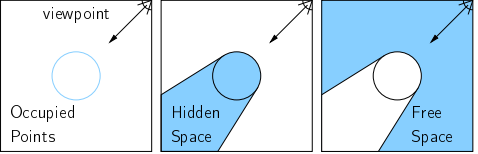
\includegraphics[width=0.9\linewidth]{\FIGDIR/10_Lidar_sets1.PNG} 
    \caption{Space type definitions}
    \label{fig:Spacetypes}
    \end{subfigure}
    \begin{subfigure}{0.5\textwidth}
    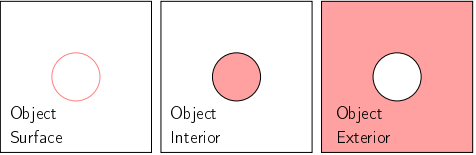
\includegraphics[width=0.9\linewidth]{\FIGDIR/11_Lidar_sets2.PNG}
    \caption{Object properties definitions}
    \label{fig:ObectProperties}
    \end{subfigure}
    \caption{Six spaces of interest \cite{yapo2008probabilistic}}
    \label{fig:Spaces of interests}
 \end{figure}
 
\noindent  Because of real-time obstacle avoidance it is necessary to introduce following terminology:
 \begin{enumerate}
 \item \textit{Occupied points} - points which have been detected by LiDAR (also addressed as visible points).
 \item \textit{Hidden space} - space which is hidden behind occupied points, from viewpoint it is uncertain what is in that space. 
 \item \textit{Free space} - space which is visible from viewpoint and it is not occupied by known objects.
 \item \textit{Object surface} - detected and undetected object surface
 \item \textit{Object interior} - occupied space by object.
 \item \textit{Object exterior} - free space around known objects.
 \end{enumerate}
 Existing method for space segregation \cite{yapo2008probabilistic} can yeld to following definition.
 \begin{definition}[Accessible space]\label{def:accessibleSpace}
    Consider known space $S$ as space explored by sensor (it can have different viewpoint along previous 3D trajectory).
    Intersection between \textit{object exterior} $S_E$ and \textit{free space}$S_F$ gives us \textit{Accessible space}.
    \begin{equation}
        S_A = S_E \cap S_F
    \end{equation}
 \end{definition}
 
 \noindent Accessible space $S_A$ (\ref{def:accessibleSpace}) is our bordering limitation for reachable space of system $R(\tau,t_0,\vec{x_0})$ (def. \ref{def:reachset01}.); 
\chapter {Detailed problem formulation}\label{ch:problemFormulation3D}
\section{Introduction}\noindent
Given a partially known world, a mission plan, and a small UAV equipped with a LiDAR sensor derive a safe and approach to real-time reactive obstacle avoidance strategy with a small computational footprint compatible with the low computational power available in small UAVs. The main application consists of terrain avoidance for low altitude flights. Following assumption holds:

\noindent
Following issues need to be addressed in practical implementation:
\begin{enumerate}
    \item \textit{Address thick data flow from LiDAR sensor} through Field Of Vision segmentation.
    \item \textit{Derive fast approximation of the reach space $R[\tau,t_0,\vec{x}_0]$ assessment} based on numeric approximation of linearized model.
    \item \textit{Real-time assessment of avoidance situation} based on reachable space $R[\tau,t_0,\vec{x}_0]$ and global goal $\mathscr{WP}_{goal}$.
    \item \textit{Determine escape route in reachable space $R[\tau,t_0,\vec{x}_0]$ search} via expanding search tree.
\end{enumerate}
\noindent
The integration of the proposed reactive obstacle avoidance framework into a UAV flight control framework is described next with reference to Figure \ref{fig:ControlConcept}, similar to $\mathscr{FOV}_{2D}$ and holds its validity:
\begin{itemize}
    \item The \textit{Emergency avoidance module} is invoked to override the trajectory tracking controller when a safety condition is violated.
    \item The \textit{Control strategy switch} will override control input of system and starts avoidance maneuver to achieve \textit{reactive avoidance}.
\end{itemize}
\newpage\noindent
Functional decomposition of the reactive obstacle avoidance framework similar to $\mathscr{FOV}_{2D}$ holds its validity:
\begin{enumerate}
    \item \textit{Obstacle Assessment} - FOV is separated into three subspaces: \textit{free space} – space which is directly visible from the vehicle and does not contain an obstacle, \textit{obstacle space} – space which is directly visible from vehicle and contains an obstacle and \textit{Uncertain space}  space in which direct visibility is hindered by obstacle.
    \item \textit{Reachable space assessment} –- free space can be divided into reachable space, which is reachable with system controls and unreachable space.
    \item \textit{Goal determination} –- within a reachable space local goal for path search is determined, safety margins and turn back maneuver are considered.
    \item \textit{Avoidance path}  calculation via an expanding search tree.
    \item \textit{Avoidance execution} via movement automaton.
\end{enumerate}

\section{Simple plane model}\label{sec:3DsimplisticplaneModel}
\noindent For avoidance theorem formulation in three dimensional space simplified rigid body kinematic model will be used. This model have decoupled roll, yaw and pitch angles which enables to provide simpler and more clean control (e.g movements can be simplified). 

\begin{equation}\label{eq:simple3dStatevector}
    \vec{x} = \left [ x_v,y_v,z_v,\alpha_v,\beta_v,\gamma_v \right ]^T
\end{equation}
State vector (\ref{eq:simple3dStatevector}) defined as positional state in euclidean position in right-hand euclidean space, where $x_v, y_v,z_v$ states, for latitude, longitude and altitude. Orientation angles for vehicle are $\alpha\beta,\gamma$ for roll, pitch, yaw angle.
\begin{equation}\label{eq:simple3dInputVector}
    \vec{u} = \left [ v, \omega_{\alpha_v}, \omega_{\beta_v},\omega_{\gamma_v}\right ]^T
\end{equation}
Input vector (\ref{eq:simple3dInputVector}) is defined as frontal velocity of vehicle $v$,orientation change in main axes as angular speed $\omega_{\alpha_v},\omega_{\beta_v},\omega_{\gamma_v}$
\begin{equation}\label{eq:simple3dvelocityDistribution}
    \begin{bmatrix}
    v_x\\
    v_y\\
    v_z\
    \end{bmatrix}
    = R_{XYZ}(\alpha_v,\beta_v,\gamma_v)
    \begin{bmatrix}
    v\\
    0\\
    0
    \end{bmatrix}
    =
    \begin{bmatrix}
        f_{v_x}(v,\alpha_v,\beta_v,\gamma_v)\\
        f_{v_y}(v,\alpha_v,\beta_v,\gamma_v)\\
        f_{v_z}(v,\alpha_v,\beta_v,\gamma_v)\\
    \end{bmatrix}
    =
    \begin{bmatrix}
         v\cos(\beta_v)\cos(\gamma_v)\\
         v\cos(\beta_v)\sin(\gamma_v)\\
         -v\sin(\beta_v)\\
    \end{bmatrix}
\end{equation}
Velocity distribution function (\ref{eq:simple3dvelocityDistribution}) is is defined trough standard rotation matrix (\ref{eq:xyzspaceRotationMatrix}) and frontal velocity $v$, final distributed velocity is time depending function with values $v_x$, $v_y$, $v_z$ given by functions $f_{v_x}(\dots)$, $f_{v_y}(\dots)$,$f_{v_z}(\dots)$. Final nonlinear model which have been derived from reference model \cite{stevens2015aircraft} is defined by (\ref{eq:simple3ddifferentialequations}).\\
\begin{equation}\label{eq:simple3ddifferentialequations}
    \begin{aligned}
        \dot{x}_v &= v_x  =f_{v_x}(v,\alpha_v,\beta_v,\gamma_v) = v\cos(\beta_v)\cos(\gamma_v)\\
        \dot{y}_v &= v_y  =f_{v_y}(v,\alpha_v,\beta_v,\gamma_v) = v\cos(\beta_v)\sin(\gamma_v)\\
        \dot{z}_v &= v_z  =f_{v_z}(v,\alpha_v,\beta_v,\gamma_v) = -v\sin(\beta_v)\\
        \dot{\alpha}_v &= \omega_{\alpha_v}\\
        \dot{\beta}_v &= \omega_{\beta_v}\\
        \dot{\gamma}_v &= \omega_{\gamma_v}\\
    \end{aligned}
\end{equation}   

\newpage
\section{Optimal trajectory planning}
\noindent Avoidance execution takes place in avoidance grid area $\mathscr{A}(t_d)$, where $t_d$ is decision time. Because Movement automaton $\mathscr{MA}$ is used to control plant, this problem can be addressed by discrete search function. Problem can be vaguely formulated as path finding in constrain-ted field of vision. Obstacles and system maneuverability is main constraint. For this part duality, between optimal path and reach sets will be relaxed. Reach set for this section guarantees only existence of trajectory. Reach set method used in section \ref{s:maxReachSet}. guarantees existence of minimal solution, because of reach set and trajectory duality.


\subsection{Optimal control problem formulation}
\noindent\textit{Performance functional} is given as standard cost function formulation for energy consumption line integral of trajectory $[x(t),y(t),z(t)]$ and line integral of steering input $[\beta_v(t),\gamma_v(t)]$  and for penalisation coefficients of steering $[c_\beta,c_\gamma]$ is in continuous time t given as: 
\begin{equation}\label{eq:j01}
    J_S(\vec{x},\vec{u})= \int_{t_0}^{\tau} \sqrt{\dot{x}_v(t)^2 + \dot{y}_v(t)^2 + \dot{z}_v(t)^2} + \sqrt{c_\beta\dot{\beta}_v(t)^2+c_\gamma\dot(\gamma)_v(t)^2} \quad \text{d}t
\end{equation}
For movement automaton sequence $B=\{m_1(t_1),\dots,m_k(t_k)\}$ the trajectory equivalence definition holds similarity property, therefore partially continuous signal generated by execution of movement buffer $B$ at movement automaton $\mathscr{MA}$ is equal to continuous signal given by $u(t)$. Moreover state in case continuous control $x(t)$ is equal to state generated by movement automaton $\mathscr{MA}$. One can rewrite (\ref{eq:j01}) for sequence of movements as $B=\{m_1(t_1),\dots,m_k(t_k)\}$ like follows:
\begin{equation}\label{eq:j02}
    J_S(\vec{x},\vec{u})= \sum_{k=1}^n \int_{t_{k-1}}^{t_{k}} \sqrt{\dot{x}_v(t)^2 + \dot{y}_v(t)^2 \quad \text{d}t + \dot{z}_v(t)^2} + \sqrt{c_\beta\dot{\beta}_v(t)^2+c_\gamma\dot(\gamma)_v(t)^2} \quad \text{d}t
\end{equation}
Execution of movements creates discrete time trail $\{\tau_0,\tau_1,\dots,\tau_k\}$, which marginalizes every time of movement execution start and end. Therefore movement $m_k(t_k)$ have execution period given as $(\tau_{k-1},\tau_k]$. Where $\tau_i$ is discete movement execution time. With some loss of precision one can rewrite (\ref{eq:j02}) as:
\begin{equation}\label{eq:j03}
    J_D(\vec{x},\vec{u}) = \sum_{k=1}^n \sqrt{\begin{aligned}
        &\left(x_v(\tau_{k})-x_V(\tau_{k-1)})\right)^2\\
        +&\left(y_v(\tau_{k})-y_V(\tau_{k-1)})\right)^2\\
        +&\left(z_v(\tau_{k})-z_V(\tau_{k-1)})\right)^2
    \end{aligned}}
    + \sum_{k=1}^n \sqrt{
    \begin{aligned}
        &c_\beta\left(\beta_v(\tau_{k})-\beta_v(\tau_{k-1})\right)^2\\
        +&c_\gamma\left(\gamma_v(\tau_{k})-\gamma_v(\tau_{k-1})\right)^2
    \end{aligned}}
\end{equation}
In given form equation $eq:j03$ uses only norm of distance and steering vectors differentials in execution time $t\in(\tau_{k-1},\tau_{k}]$. For unit movements $m_k\in M$ cost functional for trajectory $f(\dots)$ and cost functional for steering $g(\dots)$ can be proposed:
\begin{equation}\label{eq:j04}
    J_D(\vec{x},\vec{u}) = \sum_{k=1}^n f(m_k,\vec{x}_k,\vec{x}_{k-1}) + g(m_k,\vec{x}_k,\vec{x}_{k-1},c_\beta,c_\gamma)
\end{equation}
Functional $f(\dots)$ yields similar values for movement $m_k$ independent of his order in movement sequence $B$, therefore it can be approximated by mapping function $\hat{f}(mi)$:
\begin{equation}\label{eq:apff}
    f(m_k,\vec{x}_k,\vec{x}_{k-1})= \sqrt{\begin{aligned}
        &\left(x_v(\tau_{k})-x_V(\tau_{k-1)})\right)^2\\
        +&\left(y_v(\tau_{k})-y_V(\tau_{k-1)})\right)^2\\
        +&\left(z_v(\tau_{k})-z_V(\tau_{k-1)})\right)^2
    \end{aligned}}
    \sim \hat{f}(m_k)
\end{equation}
Functional $g(\dots)$ yields similar values for movement $m_k$ independent of his order in movement sequence $B$, therefore it can be approximated by mapping function $\hat{g}(m_k)$:
\begin{equation}\label{eq:apfg}
    g(m_k,\vec{x}_k,\vec{x}_{k-1},c_\beta,c_\gamma) = \sum_{i=1}^k \sqrt{
    \begin{aligned}
        &c_\beta\left(\beta_v(\tau_{k})-\beta_v(\tau_{k-1})\right)^2\\
        +&c_\gamma\left(\gamma_v(\tau_{k})-\gamma_v(\tau_{k-1})\right)^2
    \end{aligned}}
    \sim \hat{g}(m_k)
\end{equation}
Cost function (\ref{eq:j03}) is equivalent to cost function (\ref{eq:j04}). Transition period in simple systems like (\ref{eq:simple3ddifferentialequations}). \textit{Dynamic movement primitives} $p_i$ have minimal impact on system state $\vec{x}(t)$ and system input $\vec{u}(t)$ have minimal impact on movement cost $m_k(t_k)$ cost. With approximation functional $\hat{f}(\dots)$ (\ref{eq:apff}) and $\hat{g}(\dots)$ (\ref{eq:apfg}), cost function (\ref{eq:j04}) can be written as:
\begin{equation}\label{eq:j05}
    \hat{J}_D(\vec{x},\vec{u}) = \sum_{k=1}^n \hat{f}(m_k) + \hat{g}(m_k)
\end{equation}
For system given by (\ref{eq:simple3ddifferentialequations}) it is possible to show that continuous cost $J_S$ (\ref{eq:j01}), discrete cost $J_D$ (\ref{eq:j03}) and approximated discrete cost $\hat{J}_D$ (\ref{eq:j05})are equal:
\begin{equation}
    J_S(\vec{x},\vec{u}) \sim J_D(\vec{x},\vec{u})\sim \hat{J}_D(\vec{x},\vec{u}) = \sum_{k=1}^n \hat{f}(m_k) + \hat{g}(m_k)
\end{equation}

\noindent\textit{Constraints} are given by reachable space in avoidance grid $\mathscr{A}(t_0)$. Let $\mathscr{R}(t_0,\vec{x}_0)\subseteq \mathscr{A}(t_0)$ be reachable space at beginning of avoidance. Cell $c_g\in\mathscr{R}(t_0,\vec{x}_{0})$ is reachable cell and it has been determined as goal of avoidance. At initial state $\vec{x}(t_0)$ at decision time $t_d$. For trajectory $\mathscr{T}(B,c_0)$ there is sufficient control constraint given by $\mathscr{T}(B,t_0)\in \mathscr{R}(t_0)$. Therefore movement chain $B\in M^k$ given as series of movements $\{m_1(t_1),\dots,m_k(t_k)\}$ is constrained by following constraint:
\begin{equation}
    \left\{\mathscr{A}(t_0)-\mathscr{R}(t_0,\vec{x}_0)\right\} \cup \mathscr{T}(B,\vec{x}_0) = \{\},\quad B\in M^k
\end{equation}
\noindent Because cell $c_g$ is member subspace of reachable set $\mathscr{R}(t_0,\vec{x}_0)$. Trajectory existence from initial state $\vec{x}(t_0)$ to space occupied by goal cell $c_g$ is guaranteed.
\textit{Stop condition} for trajectory search is reaching center of cell $[x_c,y_c,z_c]$ with system position:
\begin{equation}
    \norm{[\vec{x}_g - \vec{x}(\tau_k)]} \le d_{stop},\quad \vec{x}(\tau_k)\in\mathscr{T}(x_0).
\end{equation}
Where $\vec{x}_g$, is center of cell $c_g$, $\vec{x}(\tau_k)$ is system position on trajectory $\mathscr{T}(B,\vec{x}_0)$ after execution of buffer $B={m_1,\dots,m_k}$ at time $\tau_k$.

\textit{Initial state} is equal to system initial state at time of decision $\vec{x}_0=\vec{x}(t_0)=\vec{x}(t_d)$. Initial input state is equal to input state at time of decision $\vec{u}_0=\vec{u}(t_0)=\vec{u}(t_d)$.

\textit{Control constraint} for system maximal steering angles are given: 
\begin{equation}
    \beta_v(t)\in [\beta_{min},\beta_{min}]    
\end{equation}
\begin{equation}
    \gamma_v(t)\in [\gamma_{min},\gamma_{min}]    
\end{equation}
\newpage\noindent \textit{Problem formulation} is stated like follow:
\begin{itemize}
    \item For system given by $\dot{x} = f(\vec{x},\vec{u})$ with initial state $x_0$ and control $\vec{u}_0$.
    \item Find optimal trajectory $\mathscr{T}(B,\vec{x}_0)$ which stays in reach set $\mathscr{R}(t_0,\vec{x}_0)$ and reaches goal cell $c_g$.
    \item Minimize cost functional $\hat{J}_D(\vec{x},\vec{u})$.
    \item With given control constraints and movement automaton $\mathscr{MA}$ as control.
\end{itemize}
Trajectory search problem can be simplified to movement buffer search $B\in M^k$ which holds constraints of state and input. 

\subsection{Minimum principle}
\noindent Reach set $\mathscr{R}(t_0,\vec{x}_0)$ guarantees that at least one solution exists. Reach set $\mathscr{R}(t_0,\vec{x}_0)$ is closed compact set within state space $\vec{x}\in\R^n$, therefore amount of trajectories $\mathscr{T}(B,\vec{x}_0)$ is finite. Not every trajectory $\mathscr{T}(B,\vec{x}_0)$ ends in goal cell $c_g\in\mathscr{A}(t_i)$. Each trajectory $\mathscr{T}$ is defined by buffer $B$, which contains chain of movements $\{m_1(t_1),\dots,m_k(t_k)\}$. Let say that $i$ is maximal count of movements to escape reach set $\mathscr{R}(t_0,\vec{x}_0)$. Then length of movement chain $B$ have following property:
\begin{equation}
    B=\{m_1(t_1),\dots,m_k(t_k)\},\quad|B|\le i
\end{equation}
With preposition that permutation set of movement buffers, in given constraint have finite count of members, e. g. is countable, standard permutation technique can be used to obtain  minimal trajectory. Depending on avoidance grid size $\mathscr{A}(t_i)$ this can take factorial amount of computation time.

Original cost function $\hat{J}_D$ (\ref{eq:j05}) does not contain terminal cost. If expected terminal cost is introduced standard A* search function can be used. Depending on implementation A* search can achieve logarithmic complexity and its more feasible for on-line optimisation. Let say that trajectory $\mathscr{T}(B,x_0)$ brings system to state $x(\tau_k)$, position of this state is given by $\vec{p}_v=[x_\tau,y_\tau,z_\tau]$ and center of goal cell $c_g$ is given as $\vec{p}_g=[x_g,y_g,z_g]$. then terminal cost of system at time $\tau_k$ is given:
\begin{equation}\label{eq:j06}
    J_T(\vec{x},\vec{u},c_g) = \norm{\vec{p}_v-\vec{p}_g}
\end{equation}
Final cost function is given as combination travel cost function $\hat{J}_D(\vec{x},\vec{u})$(\ref{eq:j05}) and terminal cost function $J_T(x,u,c_g)$ (\ref{eq:j05}). One can write final cost functional as:
\begin{equation} \label{eq:j07}
    J(\vec{x},\vec{u},c_g) = \norm{\vec{p}_v-\vec{p}_g} + \sum_{k=1}^n \hat{f}(m_k) + \hat{g}(m_k)
\end{equation}
Minimum principle implementation for (\ref{eq:j07}) cheapest path search is given by following section.

\subsection{Rapid exploraiton path search}
\noindent Rapid path exploration method is method for finding feasible paths in known environment based on limited system dynamics $\dot{x}=f(\vec{x},\vec{u})$ where input belongs to control  set $\vec{u}(t)\in U(T)$, example can be seen in figure \ref{fig:58rapidPathExploaation}.
\begin{figure}[H]
    \centering
    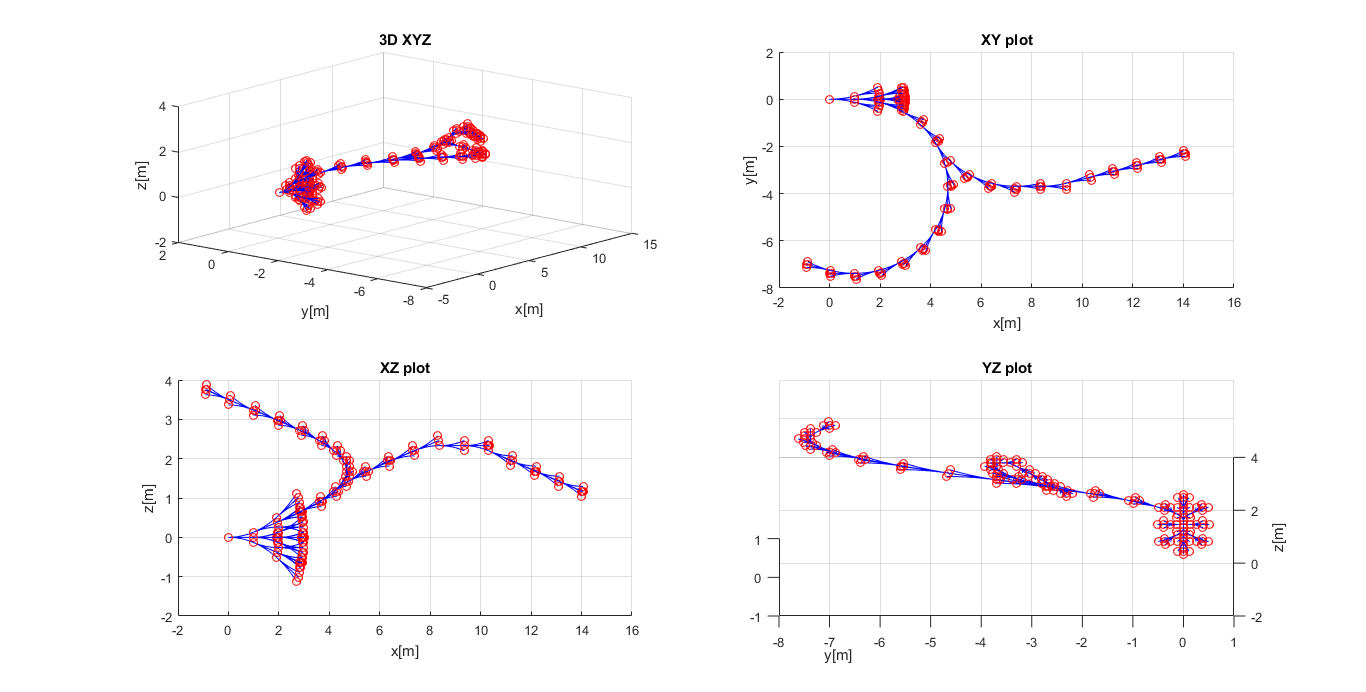
\includegraphics[width=\linewidth]{\FIGDIR/58_Rapid_exploration_path_tree.png}
    \caption{Rapid path exploration tree example with cost function $\hat{J}_D$(\ref{eq:j07}).}
    \label{fig:58rapidPathExploaation}
\end{figure}
\noindent Algorithm is based on tree search of possible movement nodes which represents vehicle state snapshots $x(t_i) i\in \N^+$. State snapshots are calculated based on predictive or linear model, to save computation time and calculation guarantees that real vehicle state $\hat{x}(t_i)$ will reach  state $\vec{x}(t_i)$ with small perturbation $\epsilon$ therefore for each predicted state following inequality holds:
\begin{equation}\label{eq:marginalErrorofPrediction}
    \norm{\hat{x{t_i}}-\vec{x}(t_i)}\le \epsilon^i,\quad i \in \N^+
\end{equation}
\noindent All possible trajectories $\mathscr{T}$ in search tree are represented as sequence of nodes. Each node have defined parent, which is reference to previous node and leafs which are references to possible followers in path. For our purpose augmented data structure \textit{Node} will be presented with following properties:
\begin{enumerate}
    \item \textit{Movement} - movement which has been executed on this node.
    \item \textit{Goal distance} - distance to goal point in space calculated by (\ref{eq:distanceToGoalCalc}).
    \item \textit{Explored} - indication if node have been explored by stack execution true or false.
    \item \textit{Vehicle} - vehicle structure with state and obstacles situation.
    \item \textit{Parent} - parent node handle, if empty node is root of tree. 
    \item \textit{Leafs} - list of accessible non vehicle destructive leafs.
\end{enumerate}
\begin{equation}\label{eq:distanceToGoalCalc}
    d_{goal}(vehicle,\mathscr{W}_g) = 
    \begin{cases}
        \norm{\vec{x}_v-\vec{x}_{goal}}&:\nexists o \in \mathscr{O}; o.danger = 1 \vee 2\\
        \infty&:otherwise
    \end{cases}
\end{equation}
\noindent For purpose of rapid exploration limited move set needs to be introduced, therefore based on defined simplistic system model control set (\ref{simple3dControlSet}):
\begin{equation}\label{eq:rapidExplorationMovementSet}
    moveSet=
    \begin{cases}
        \left\{straight,left,right,up,down \right\} &: node.movement == straight\\
        \left\{straight,left, \right\} &: node.movement == left\\
        \left\{straight,right \right\} &: node.movement == right\\
        \left\{straight,up \right\} &: node.movement == up\\
        \left\{straight,down \right\} &: node.movement == down
    \end{cases}
\end{equation}
\noindent Goal of rapid exploration is to cover maximum amount of space without redundancy therefore allowed movement set \ref{eq:rapidExplorationMovementSet} is covering this situation. For example movement series $[right,left]$ returns to path given by movement series $[straight,straight]$, therefore possible movements after i finis $right$ movement are $right,straight$. This rule reduces search tree complexity from branching factor $n^5$ to branching factor $n^3$. Expand function represented by algorithm \ref{alg:03}.

\begin{algorithm}[H]
\caption{Node expand(...) function.}
\label{alg:03}
\SetKwInOut{Input}{Input}\SetKwInOut{Output}{Output}
\Input{Node node}
\Output{Node[] leafs}
\If{isEmpty(node.leafs)}{
    \ForEach{$appliedMovement\in \left\{straight,left,right,up,down \right\}$}{
        newVehicle = vehicle.predictPosition(appliedMovement);\\
        Node child = new Node(vehicle);\\
        child.recalculateDistance();\\
        child.parrent = node;\\
        node.leafs.append(child);
    }
}
\end{algorithm}
\noindent Node selection is executed based on algorithm \ref{alg:04}. Not all leafs of expanded node can be exploration candidates, because some movements can lead to vehicle crash, which is represented by $node.goalDistance = \infty$. Other reason to decline leaf as exploration candidate is inappropriate movement, movement set which is based on parent node movement (\ref{eq:rapidExplorationMovementSet}), can allow only certain candidates to be explored. Other selection criteria based on system dynamics or constraints can be introduced into selection function later.

\begin{algorithm}[H]
    \caption{Node select(...) function.}
    \label{alg:04}
    \SetKwInOut{Input}{Input}\SetKwInOut{Output}{Output}
    \Input{Node node}
    \Output{Node[] candidates}
    candidates = [];\\
    \ForEach{leaf $\in$ node.leafs}{
    \If{leaf.movement $\in$ moveSet and leaf.goalDistance $\neq \infty$ and\\
        leaf.goalDistance $\le$ node.goalDistance and leaf.explored == false}{
            leaf.explored = true;\\
            candidates.append(leaf);
    }
}
\end{algorithm}
\noindent Stack structure search is used for heuristic search of optimal path according to cost function (\ref{eq:j07}). Path given by heuristic algorithm \ref{alg:05}. is semi-optimal strongly depending on chosen time interval $t_i$ for prediction, count of predicted states $i$ and acceptable marginal error of prediction (\ref{eq:marginalErrorofPrediction}). 
\begin{algorithm}
    \caption{Search path function.}
    \label{alg:05}
    \SetKwInOut{Input}{Input}\SetKwInOut{Output}{Output}
    \Input{Node root, $\mathscr{WP}$ goal}
    \Output{Node path}
    stack = [root];
    \While{~isEmpty(stack)}{
        node = findBestCandidate(stack,goal); (\ref{eq:j07})\\
        node.expand($\dots$); (alg. \ref{alg:03}.)\\
        candidates = node.select($\dots$); (alg. \ref{alg:04}.)\\
        \ForEach{candidate $\in$ candidates}{
            \If{candidate.distance(goal) $\le$ marginDistance}{
                return candidate;
            }
        }
    }
\end{algorithm}

\chapter{Control approach}\label{ch:controlapproach3D}


\section{Control strategy}\label{sec:3DcontrolSimplisticStrategy}
\noindent Main purpose of control strategy is to define discrete set of moves which can be later used in approximation models. Therefore vehicle velocity is set to constant speed $v_v = 1\quad m/s$ because increasing and decreasing speed can make predicted trajectories malformed. It is needed to distinguish between \textit{control strategy} $\Omega(t)$ and \textit{control set} $U(t)$. \textit{Control set} $U(t)$ contains all available control inputs regardless vehicle state and surrounding. \textit{Control strategy} $\Omega(t)$ contains only control inputs $\omega(t)$ which keeps vehicle in safe invariant reachable set $\mathscr{R}$.
\begin{equation}\label{simple3dControlSet}
    u(t)\in U(T) =
    \begin{cases}
        \left [ v_c,0,0,0 \right ]^T & :s_0 \quad\textnormal{fly straight} \\
        \left [ v_c,0,\frac{\pi}{12},0 \right ]^T & :s_1 \quad\textnormal{fly downward} \\
        \left [ v_c,0,-\frac{\pi}{12},0 \right ]^T & :s_2 \quad\textnormal{fly upward} \\
        \left [ v_c,0,0,\frac{\pi}{12} \right ]^T & :s_3 \quad\textnormal{fly left} \\
        \left [ v_c,0,0,-\frac{\pi}{12} \right ]^T & :s_4 \quad\textnormal{fly right} 
    \end{cases}
\end{equation}
Control set $U(t)$ (\ref{simple3dControlSet}) contains five basic movement which affects yaw or pitch angular velocity. This allows us to develop movement set containing basic movement like fly straight, fly upward, fly downward, fly left and fly right. Movement set  is designed to cover maximum maneuverability. From viewpoint of reachable control set $U(t)$ have maximal maneuverability subset $\Gamma(t)$ which contains only maneuvers which are on border of reach set. Maximal maneuverability subset $\Gamma(t)$ is equal to control set $U(t)$ in this case. For example les sharp turn to right $u(t)=\left [ v_c,0,0,-\frac{\pi}{16} \right ]^T$ will be member of control set $U(t)$, but will not be member of maximal maneuverability set $\Gamma(t)$, because there exist sharper turn to right $u(t) = \left [ v_c,0,0,-\frac{\pi}{12} \right ]^T $. Maximal maneuverability set $\Gamma(t)$ is used in estimation of invariant safe reach set $\mathscr{R}$.

\newpage
\section{Path finding in partially known environment}
\noindent Path finding in partially known environment is nontrivial task which requires additional safety margin. Firstly visibility field $\mathscr{F}_{3D}$ needs to be defined for single time snapshot, then it can be extended to trajectory.
\subsection{Visibility field}
\begin{definition}{Visibility field in third dimension $\mathscr{F}_{3D}$}\label{def:VisibleSpace}
    Let $x_0=[0,0,0]^T$ be observation point and X axis as directional axis, horizontal view limiter on XY plane as $[\theta_S,\theta_E]$, vertical view limiter on XZ plane as $[\varphi_S,\varphi_E]$ and view distance as $d_v$.
    \\
    Then point $x_p=[x,y,z]\in R^3$ with horizontal angle $\theta_p = \arctan y/x$, vertical angle $\varphi_p=\arctan z/x$  and $d_p=\norm{x_p}$ belongs to visibility field if and only if:
    \begin{equation}
        0 \le d_p \le d_v
    \end{equation}
    \begin{equation}
        \theta_S \le \theta_p \le \theta_E
    \end{equation}
    \begin{equation}
        \varphi_S \le \varphi_p \le \varphi_E
    \end{equation}
\end{definition}
\noindent\textit{Visibility field} $\mathscr{F}_{3D}$ can be divined into \textit{visibility grid} $\mathscr{G}_{3D}$ to ease computational complexity, this approach is taken from \cite{goerzen2010survey}. This approach is based on fast classification of obstacle space $\mathscr{O}_{3D}$ and uncertain space $\mathscr{U}_{3D}$ in field of vision $\mathscr{F}_{3D}$. Cell size can be scaled to needs of path finding algorithm.
\begin{definition}{Visibility grid cell $c_{i,j,k}\in\N^+$}\label{def:visibilityGridCell}
    in grid is with defined position by layer index $k\in\{1\dots l_c\}$, column index $j\in\{1\dots h_c\}$ and  row index $i\in\{1\dots v_c\}$, where $l_c\in\N^+$ is layer count, $v_c\in\N^+$ is vertical cell count, $h_c\in\N^+$ is horizontal cell count. Example of grid cell can be found in figure \ref{fig:62VisibilityGridCellExample}.
    \begin{figure}[H]
        \centering
        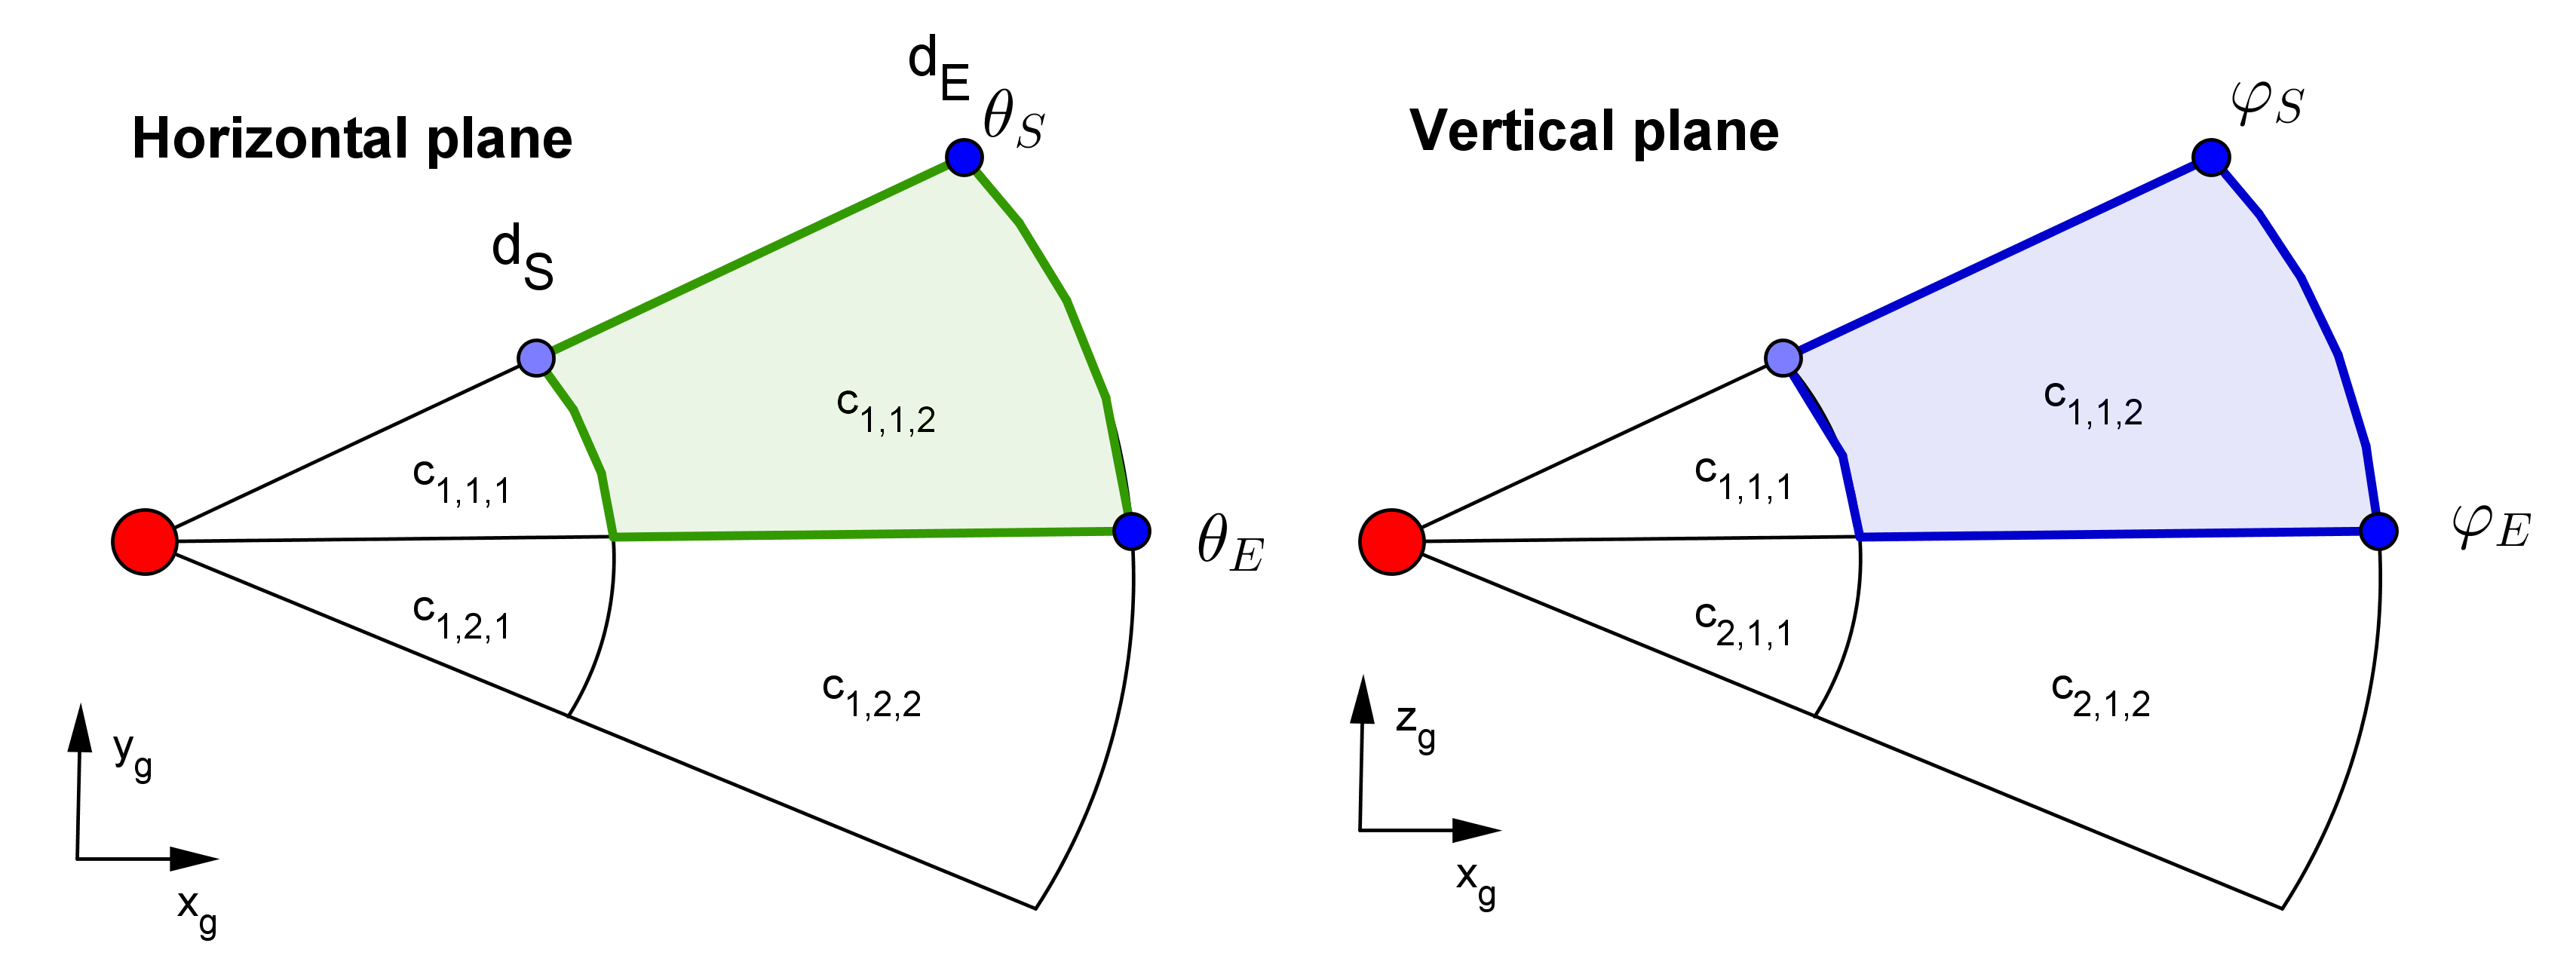
\includegraphics[width=0.8\linewidth]{\FIGDIR/62_Visibility_Grid_Cell_example.png}
        \caption{Visibility grid cell $c_{1,1,2}$ example.}
        \label{fig:62VisibilityGridCellExample}
    \end{figure}
    Visibility grid cell occupied space is defined by $[d_s,d_e,\theta_s,\theta_e,\varphi_s,\varphi_e]$, where $(d_s,d_e]\in\R^2$ distance range, $(\theta_s,\theta_r$ is horizontal range and $(\varphi_s,\varphi_e]$ is vertical range. Then point $x_p=[x,y,z]\in R^3$ with horizontal angle $\theta_p = \arctan y/x$, vertical angle $\varphi_p=\arctan z/x$  and $d_p=\norm{x_p}$ belongs to visibility grid cell $c_{i,j,k}\in\N^+$ if and only if:
    \begin{equation}
        d_s \le d_p \le d_e
    \end{equation}
    \begin{equation}
        \theta_s \le \theta_p \le \theta_e
    \end{equation}
    \begin{equation}
        \varphi_s \le \varphi_p \le \varphi_e
    \end{equation}
    \newpage\noindent    
    Visibility grid cell have defined state property s:
    \begin{enumerate}
        \item \textit{Not determined} - state of cell have not been determined, because it does not complain with any following status rule.
        \item \textit{Reachable} - cell is reachable and there exist control input $u(t)$ which will bring position state $[x_p(t),y_p(t),z_p(t)]^T$ to any point belonging to cell from grid origin $[0,0,0]^T$, and any point of trajectory $[x_p(t),y_p(t),z_p(t)]^T$ does not belong to grid cell with Obstacle or Uncertain state.
        \item \textit{Unreachable} - cell is unreachable and there does not exist any control input $u(t)$ which comply with reachibility rule.
        \item \textit{Obstacle} - cell contains at least one detected obstacle point from obstacle set $\mathscr{O}_{3D}$.
        \item \textit{Uncertain} - cell visibility is hindered by obstacle cell or uncertain cell on previous layer.
        \item \textit{Goal} - cell center is closest to goal waypoint $\mathscr{WP}_{goal}$.
    \end{enumerate}
    \textit{Successors} is set of cells directly or partially covered in line of sight by selected cell $c_{i,j,k}$. \textit{Predecessors} is set of cells directly or partially covering line of sight of selected cell $c_{i,j,k}$.
\end{definition}
\noindent For  further definition of partially known environment definitions of  visibility grid (\ref{def:VisibleSpace}), visibility grid cell (\ref{def:visibilityGridCell}), local obstacle position transformation (\ref{def:globalObstaclePosition3D}). Let say that system $\dot{x} = f(x,u)$ finishes scanning of surrounding environment at time $t_i$ in visibility grid defined by  parameters $[d,\theta_S,\theta_E,\varphi_S,\varphi_E,l_c,h_c,v_c]$. Then $\mathscr{F}_{3d}(t_i)$ gives situation valid for small time frame $[t_i,t_{i+1})$, where $t_{i+1}$ is time of new full surrounding environment scan. 

In this operational frame three distances are setup $0 \le d_p \le d_o \le  d_u \le d$ where $d_p$ is processing distance, $d_o$ is operational distance and $d_u$ is unsafe distance. Processing distance $d_p$ is is maximal distance in which avoidance maneuvers are processed. Operational distance $d_o$ is distance in which  any avoidance maneuver is safe. Unsafe distance $d_u$ is a distance in which avoidance maneuver may lead to crash. Example of avoidance frame overlapping can be found in figure \ref{fig:visibleVsReachableLocalFrame}. Following assumptions have been taken into account:

\begin{assumption}{Processing distance $d_p$ is equal to 0, therefore result of avoidance engine is known at time of detection $t_i$.}\label{ass:7}\end{assumption}
\begin{assumption}{Unsafe distance $d_u$ is equal to visibility distance $d$.}\label{ass:8}\end{assumption}
\noindent For better imagination what this assumptions have done on presented avoidance principle is summarized in following outcome of assumptions \ref{ass:7}. and \ref{ass:8}:
\begin{enumerate}
    \item Avoidance area $\mathscr{A}(t_i)$ is equal to visibility field $\mathscr{F}_{3D}(t_i)$.
    \item There is no unsafe area because $d_u=d$.
    \item Controlable origin (point where you can change vehicle trajectory) is at origin of $\mathscr{F}_{3D}$.
\end{enumerate}

\subsection{Pre-calculated reach set approach}
\noindent To minimize computation time of reachable space for system $\dot{x}=f(x,u)$, with movement automaton $\mathscr{MA}$ given by definition \ref{def:movementAutomaton} in Visibility grid $\mathscr{G}_{3D}$ given by definition \ref{def:VisibleSpace} partitioned into visibility cells $c_{i,j,k}\in \mathscr{G}_{3D}$ given by definition \ref{def:visibilityGridCell} two stage computation method is presented. 
\begin{enumerate}
    \item \textit{First stage} is to create numeric approximation of Reach set in $\mathscr{G}_{3D}$ where all visibility grid cells are considered as \textit{Not determined} state.
    \item \textit{Second stage} is to use pre-calculated structure and prune it with \textit{Obstacles} and \textit{Uncertain} cells popping in.
\end{enumerate}
 This approach allows us to use heavy computational methods in first stage and removing bias of additional calculations from second stage. Second stage is used every obstacle avoidance framework run. First stage is used only in case of following events:
\begin{enumerate}
    \item \textit{System equation change} - when system $\dot{x}=f(x,u)$ changes, this can be invoked by payload or weather condition change, prior the mission execution.
    \item \textit{Control strategy change} - when control strategy $u(t)\in U(t)$ changes, this can be invoked by control constraints change.
    \item \textit{Movement set change} - movement automaton $\mathscr{MA}$ has finite set of movements $m_i\in M$, when this set changes reach set estimation structure needs to be recalculated due the estimation method dependence. 
\end{enumerate}

\noindent\textit{Trajectory representation} is key in this approximation method. Reach set $\mathscr{R}[t_0,t_1,x_0]$ can be represented as set of all trajectories reachable from starting point $x_0$ at time $t_0$ up to end time $t_1$. Reduction of reach set from closed compact set $\mathscr{R}\subset \R^N$ to closed compact set of movement chains $\mathscr{R}\subset M^m, m\in\N^+$ is granted trough using movement automaton $\mathscr{MA}$ as control input in closed control loop for system $\dot{x} = f(x,u)$.

\begin{definition}{Trajectory $\mathscr{T}(x_0,B)$.}\label{def:movementTrajectory} 
    System given by equation $\dot{x}=f(x,u)$ with state vector $x\in \R^n$ and input vector $u \in \R^M$, where control input is $u(t)$ is generated by movement automaton $\mathscr{MA}$. Set of available movements is given by $M\in\mathscr{MA}$, where buffer $B$ ordered set of movements $m_i(t_i)\in M^k, k\in \N^+$. Input signal $\mu(t)$ is execution of movement automaton. Then trajectory $\mathscr{T}(x_0,B)$ is trajectory in state space $x\in\R^n$  executed in time $t\in [t_0,T]$. where final time is given as:
    \begin{equation}
        T= \sum_{i=0}^{k} t_i,\quad t_i\in B 
    \end{equation}
    System state equation solution is given as $\Phi(t,t_0,x_0)$, trajectory $\mathscr{T}(x_0,B)\in \R^n$ is given as:
    \begin{equation}
        \mathscr{T}(x_0,B)= \bigcup_{t\in[t_0,T]} \Phi(t,t_0,x_0)
    \end{equation}
\end{definition}
\noindent One can see that trajectory for initial state $x_0$ and movement buffer $B$ is subset of system state space $x\in\R^n$. To aproximate reach set $R[t_0,t_1,x_0]$ one needs to combine all possible system trajectories where $T\le t_1$.
\begin{definition}{Reach set $\mathscr{R}(t_0,t_1,x_0)$ approximation for system with $\mathscr{MA}$ control.}\label{def:NumericReachSet3D}
    System given by equation $\dot{x}=f(x,u)$ with state vector $x\in \R^n$ and input vector $u \in \R^M$, where control input is $u(t)$ is generated by movement automaton $\mathscr{MA}$. Let  $\mathscr{B}(t_1)$ be ordered set of all possible movement permutations of movements where execution time $T\le t_1$. Movement permutation set $\mathscr{B}(t_1)$ is given by equation:
    \begin{equation}
        \mathscr{B}(t_1) = \bigcup_{T\le t_1} \left\{ m_1(\tau_1),\dots,m_n(\tau_n)\right\};\quad m_i(\tau_i)\in M;\quad \sum_{k=1}^i \tau_i \le t_1
    \end{equation}
    With known movement permutation set $\mathscr{B}(t_1)$ and initial system state $x_0$ one can easily define $\mathscr{R}(t_0,t_1,x_0)\in \R^n$ as follows:
    \begin{equation}
        \mathscr{R}(t_0,t_1,x_0)=\bigcup_{B\in\mathscr{B_i}(t_1)} \mathscr{T}_i(x_0,B_i) 
    \end{equation}
    Where $B_i$ represents i-th movement buffer and $\mathscr{T}_i(x_0,B_i)$ represents i-th trajectory for respective buffer.
\end{definition}
\noindent This approximation of reach set is computational heavy, because movement permutation set $\mathscr{B}(t_1)$ have factorial growth depending on maximal count of movements in time-frame of $[t_0,t_1]$. On the other hand Reach set contains finite number of trajectories, which allows to implement fast pruning methods to obtain reduced reach set $\mathscr{R}_R(t_0,t_1,x_o)\subset\mathscr{R}(t_0,t_1,x_0)$. Relation between reach set and visibility field can be introduced by implementaiton of membership function. Membership function is defined for trajectory $\mathscr{T}(x_0,B)$ as follow:
\begin{definition}{Membership function $\Gamma(c_{i,j,k},\mathscr{T}(x_0,B))$.}\label{def:trajectoryMembershipFunction}
    Let $x_t$ be positional/orientation subset of $R^n$ given as touple of $[p,o]\subset \R^{lm}$, where $p$ is positional subspace with dimension $l$ in system coordinate frame and $o$ is orientation subspace with $l$ dimension in coordinate system. Therefore trajectory evolution can be extracted from trajectory $\mathscr{T}(x_0,B)$ as follow:
    \begin{equation}
        x_t = [\vec{p},\vec{o}]\subset \mathscr{B}(x_0,B)\subset \mathscr{R}(t_0,t_1,x_0)
    \end{equation}
    Grid cell $c_{i,j,k}$ occupies cell space $x_c \subset \R^l$. Therefore membership function $\Gamma(c_{i,j,k},\mathscr{T}(x_0,B))$ is deffined as follow:
    \begin{equation}
        \Gamma(c_{i,j,k},\mathscr{T}(x_0,B))=
        \begin{cases}
            \text{member} & \text{if } p \cap x_c \neq \{\}\\
            \text{void} & \text{otherwise}
        \end{cases}
    \end{equation} 
\end{definition}
\noindent Definition \ref{def:trajectoryMembershipFunction}. can be simplified as when trajectory $\mathscr{B}(x_0,B)$ position subspace intersect cell occupied space it belongs to cell $c_{i,j,k}$.Because trajectory $\mathscr{B}(T,x_0)$ is time depending, one can determine cell entrance time and cell exit time. These properties can be useful in terms of moving obstacle avoidance. Other notable property of mapping is that cells in $\mathscr{G}_{3D}$ can be ordered based on trajectory $\mathscr{T}(x_0,B)$ entrance/exit time.
\begin{definition}{Cell sequence $\mathscr{C}(\mathscr{T}(x_0,B))$.}\label{def:cellSequence}  
    Let $\mathscr{T}(x_0,B)$ by definition \ref{def:movementTrajectory} with trajectory execution time $t\in [t_0,t_1]$. Visibility grid cell $c_{i,j,k}$ belongs to visibility field of $\mathscr{G}_{3D}$. Membership function $\Gamma(c_{i,j,k},\mathscr{T}(x_0,B))$ can be extended to define membership at time $t$ as $\Gamma(c_{i,j,k},\mathscr{T}(x_0,B),t)$. Cell entrance time is given as $t_e\in [t_0,t_1]$ when $\Gamma(c_{i,j,k},\mathscr{T}(x_0,B),t) = \text{member}$ for $t=t_e$ and $\Gamma(c_{i,j,k},\mathscr{T}(x_0,B),t)=\text{void}, \forall t\le t_e$. Then cell sequence is ordered subset of $\mathscr{G_{3D}}$, with ordering by $t_e$.
    \begin{equation}
        \mathscr{C}(\mathscr{T}(x_0,B)) = \left\{c_l\in \mathscr{G}_{3D}:\Gamma(c_{l},\mathscr{T}(x_0,B),t) = \text{member}, t_{e_{l-1}} < t_{e_{l}} < t_{e_{l+1}} \right\}
    \end{equation}
\end{definition}
\noindent With cell sequence defined $\mathscr{C}(\mathscr{T}(x_0,B))$ one can easily map any trajectory to cells. To successfully merge reach $\mathscr{R}(t_0,t_1,x_0)$, with visibility grid $\mathscr{F}_3D$ some additional structures needs to be defined and some needs to be extended as follows:
\begin{enumerate}
    \item \textit{Trajectory register} - map of all trajectories $\mathscr{T}(x_0,B)\in\mathscr{R}(t_0,t_1,x_0)$, which are viable in unoccupied space with following properties:
    \begin{enumerate}[a.]
        \item \textit{Trajectory identifier} - unique sting (created from  $\mathscr{C}(\mathscr{T}(x_0,B))$). 
        \item \textit{Trajectory object} - object of trajectory $\mathscr{T}(x_0,B)$.
    \end{enumerate}
    \item \textit{Trajectory} - as given by definition \ref{def:movementTrajectory}. is extended by following properties:
    \begin{enumerate}[a.]
        \item \textit{Cell sequence $\mathscr{C}(\mathscr{T}(x_0,B))$} - list of passing cells in order, this parameter helps to remove trajectory from cell regisries and trajectory register.
        \item \textit{Trajectory cost} - cost of trajectory $J*(x(t),u(t))$ - is used by decision making algorithm to choose best viable trajectory for execution.
    \end{enumerate}
    \item \textit{Visibility grid cell} - as given by definition \ref{def:visibilityGridCell}. is extended by list of trajectories passing or ending in cell with folowing members:
    \begin{enumerate}[a.]
        \item \textit{Trajectory identifier} - unique sting (created from  $\mathscr{C}(\mathscr{T}(x_0,B))$).
        \item \textit{Trajectory intersection state} - indicates if trajectory is passing or finishing in cell.
        \item \textit{Trajectory entrance time} - time when trajectory enters to cell.
        \item \textit{Trajectory exit time} - time when trajectory leaves cell, this parameter is important in case of passing trajectiories, because execution of movement automaton $\mathscr{MA}$ needs to be cut at this time.
    \end{enumerate}
\end{enumerate}

\begin{figure}[H]
    \centering
    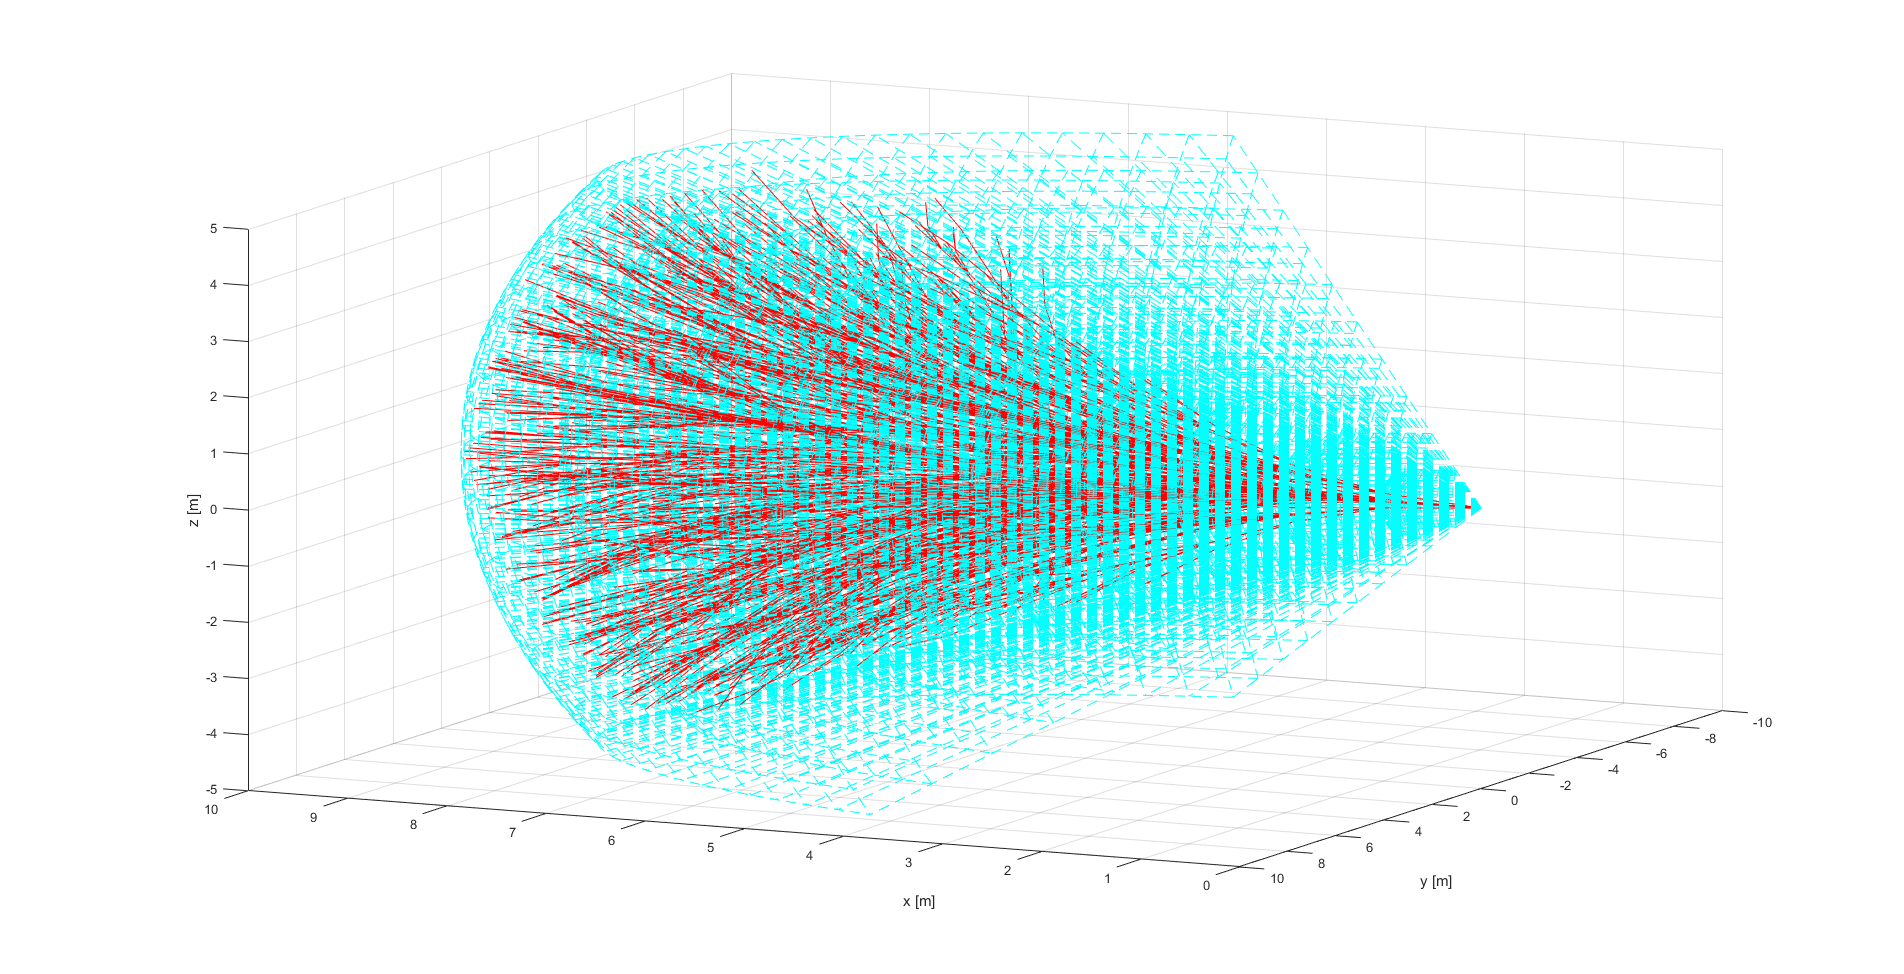
\includegraphics[width=0.95\linewidth]{\FIGDIR/41_Visible_vs_reachable_space.png}
    \caption{Comparison between reachable space and visible space in local coordinates frame.}
    \label{fig:visibleVsReachableLocalFrame}
\end{figure}
\noindent Proposed reach set estimation method have beem used on simplistic plane model from section \ref{sec:3DsimplisticplaneModel} with control strategy $U(t)$ implemented by movement automaton movement set defined in section \ref{sec:3DcontrolSimplisticStrategy}. Final reach set $\mathscr{R}(t_0,t_1,x_0)$ from definition \ref{def:NumericReachSet3D}. is portrayed in visibility grid $\mathscr{G}_{3D}$ in (fig. \ref{fig:visibleVsReachableLocalFrame}).

\subsection{Maximal reach set computation method}\label{s:maxReachSet}
\noindent The first stage of reachable space $\mathscr{R}(t_0,t_1,x_0)$ is computational heavy and its based on prediction of all possible trajectories $\mathscr{T}(x_0,B)$ from def.\ref{def:movementTrajectory}. Each trajectory is defined by movement buffer $B$ from movement automaton $\mathscr{MA}$ movement permutation set $\mathscr{B}(t_1)$ (def. \ref{def:NumericReachSet3D}.). Membership function $\Gamma(c_{i,j,k},\mathscr{T}(x_0,B))$ defined in (def. \ref{def:trajectoryMembershipFunction}.) enables to obtain cell sequence $\mathscr{C}(\mathscr{T}(x_0,B))$ defined in (def. \ref{def:cellSequence}). Cell sequence can be weaved into structure of visibility grid $\mathscr{G}_3D$. Interconnected reach set $\mathscr{R}(t_0,t_1,x_0)$ and visibility grid $\mathscr{G}_{3D}$ for time of scanning $t_i$ results into new structure of \textit{Avoidance grid} $\mathscr{A}(t_i)$. Procedure of avoidance grid creation is described in algorithm \ref{alg:firstStage}.

\begin{algorithm}[H]
    \caption{First stage - calculate maximal reach set.}
    \label{alg:firstStage}
    \SetKwInOut{Input}{Input}
    \SetKwInOut{Output}{Output}
    \Input{Vehicle initial state $x_0$,Vehicle dynamics $\dot{x}=f(x,u)$,\\ Movement Automaton $\mathscr{MA}$, Visibility grid $\mathscr{G}_{3D}$}
    \Output{Avoidance grid $\mathscr{A}(t_i)$}
    $\mathscr{A}(t_i)$=newGrid($t_i,x_0,\dot{x}=f(x,u),\mathscr{MA},\mathscr{G}_{3D}$)\;
    \ForEach{cell $c_{i,j,k}\in\mathscr{A}(t_i)$}{
        $c_{i,j,k}$.status = 'Uncertain'\;
        }
    $t_1\in \R^+$ = maximal escape time \;
    Create movement permutation set $\mathscr{B}(t_i)$\;
    \ForEach{movement buffer $B\in\mathscr{B}(t_i)$}{
        trajectory = $\mathscr{T}(x_0,B)$\;
        cellList = $\mathscr{C}(\mathscr{T}(x_0,B))$\;
        code = hash(cellList)\;
        $\mathscr{A}(t_i)$.trajectoryRegister.put(code,trajectory)\;
        trajectory.cost = trajectory.calculateCost\;
        trajectory.cellSequence=cellList\;
        \ForEach{cell $c_{i,j,k}\in$cellList}{
            state = getState(cell,trajectory)\;
            [entrance,exit] = $\Gamma(c_{i,j,k},\mathscr{T}(x_0,B))$\;
            $c_{i,j,k}$.addTrajectory(code,state,entrance,exit)\;
    }}
\end{algorithm}
\noindent Avoidance grid $\mathscr{A}(t_i)$ for avoidance time $t_i$ represents all possible avoidance trajectories $\mathscr{T}(x_0,B)$ in given visibility grid $\mathscr{G}_{3D}$. Avoidance grid have following properties:
\begin{enumerate}
    \item \textit{Trajectory bounding} - each trajectory $\mathscr{T}(x_0,B)$ in reach set $\mathscr{R}(t_0,t_1,x_0)$ is bounded by positional space occupied by visibility grid $\mathscr{G}_{3D}$.
    \item \textit{Trajectory belonging} - each part of each trajectory $\mathscr{T}(x_0,B)$ in reach set $\mathscr{R}(t_0,t_1,x_0)$ belongs each time of execution to one visibility grid cell $c_{i,j,k}\in\mathscr{G}_{3d}$.
    \item \textit{Trajectory execution-ability} - trajectory $\mathscr{T}(x_0,B)$ with movement buffer $B$ is possible to execute at avoidance time $t_i$ if and only if every cell $c_{i,j,k}$ in trajectory cell sequence is reachable.
    \item \textit{Trajectory cost} - trajectory $\mathscr{T}(x_0,B)$ has given cost of execution for each movement $m_i\in B$ by cost function $J^*(x,u)$.
\end{enumerate}

\subsection{Pruning reach set}
\noindent Second stage of algorithm is much faster than first stage (alg.\ref{alg:firstStage}.), Because it is working with pre-calculated maximal reach set $\mathscr{R}_0(t_0,t_1,x_0)$. To obtain reduced reach set $\mathscr{R}(t_0,t_1,x_0)$ pruning method is introduced in alg. \ref{alg:PruneReachSet}. Visibility grid cells $c_{i,j,k}$ have state which constraints possibilities of vehicle movement. If this status is restrictive, like the cell is \textit{obstacle} or visibility is hindered, therefore cell state is \textit{uncertian}, reach set must be changed to reflect cell status. Trajectory $\mathscr{T}(x_0,B)$ contains movement buffer $B\in\mathscr{MA}$, therefore trajectory can be considered as chain of decisions. Decisions which leads to cells $c_{i,j,k}$ must be removed to maintain reach set $\mathscr{R}$ consistency. Because reach set $\mathscr{R}_0$ is similar to decision tree, application of pruning is feasible \cite{esposito1997comparative}.

\begin{algorithm}[H]
    \caption{Second stage - applying pruning method.}
    \label{alg:PruneReachSet}
    \SetKwInOut{Input}{Input}
    \SetKwInOut{Output}{Output}
    \Input{Target cell for removal $c_{i,j,k}$, Avoidance Grid $\mathscr{A}(t_i)$}
    \Output{Pruned avoidance grid $\mathscr{A}(t_i)$}
    String[] trajectoryCodes = $c_{i,j,k}$.getAllTrajectoryCodes()\;
    \ForEach{code $\in$ trajectoryCodes}{
        trajectory = $\mathscr{A}(t_i)$.getTrajectory(code)\;
        cells = trajectory.cellSequence()\;
        $\mathscr{A}(t_i)$.removeFromRegister(code)\;
        $\mathscr{A}(t_i)$.updateTrajectoryCount()\;
        \ForEach{cell $c_l\in$ cells}{
            $c_l$.removeTrajectory(code)\;
            $c_l$.updateTrajectoryCount()\;
        }
    }
\end{algorithm}
\noindent Because avoidance grid $\mathscr{A}(t_i)$ contains \textit{trajectory register} and each passing trajectory $\mathscr{T}$ is linked to cell $c_i,j,k$ registry. Cross object removal method must be applied. Method to prune reach set $\mathscr{R}$ (alg \ref{alg:PruneReachSet}.)  reflects this fact. Modern object oriented programming languages, like \textit{C++}, enable such implementation \cite{hill1996object}.
	
\subsection{Estimated reach set computation method}\label{ch:estimatedReachSetMethod}
\noindent Let assume that at begin of reach set $\mathscr{R}(t_0,t_1,x_0)$, set of obstacles $\mathscr{O}$ exists. Each obstacle $o\in\mathscr{O}$ is given as point in local coordinate time frame $[d_o,\theta_o,\varphi_o]$, where $d_o$ represents distance, $\theta_o$ represents horizontal angle and $\varphi_o$ represents vertical angle of matter point. Tresholding, filtering and frame shifting are already applied to raw sensor data. Pre-calculated maximal reach set $\mathscr{R}_0(t_0,t_1,x_0)$ is merged to local coordinate frame of avoidance grid $\mathscr{A}(t_i)$. Initial time in reach set is identical to $t_0=t_i$ and final time of reach set $t_1=t_i+t_1$. Initial conditions of system $x_0$ are converted from global coordinate frame to avoidance grid coordinate frame. With well defined offsets, maximal reach set $\mathscr{R}_0$ can be used for any avoidance time $t_i$ and vehicle initial avoidance state $x_i$.

Obstacle avoidance algorithm starts with \textit{initialization of avoidance grid $\mathscr{A}(t_i)$}, where status of each cells $c_{i,j,k}\in\mathscr{A}(t_i)$ status is set as 'Not determined'. For each detected obstacle point in local planar coordinates  $[d_o,\theta_o,\varphi_o]^T$ Obstacle assessment function is given by alg. \ref{alg:06}.
\\
\begin{algorithm}[H]
    \caption{Put obstacle fuction.}
    \label{alg:06}
    \SetKwInOut{Input}{Input}
    \Input{Avoidance grid $\mathscr{A}(t_i)$ grid, Obstacle point $[d_o,\theta_o,\varphi_o]^T$}
    $c_{i,j,k}$=grid.getCell($d_o,\theta_o,\varphi_o$)\;
    \If{$c_{i,j,k}$.status != 'Obstacle'}{
        $c_{i,j,k}$.status = 'Obstacle'\;
        prune($c_{i,j,k}$,${A}(t_i)$)\;
        successors = $c_{i,j,k}$.successors\;
        \ForEach{s $\in$ successors}{
            s.status = 'Uncertain'\;
            prune(s,${A}(t_i)$)\;
        }
    }
\end{algorithm}
\noindent\textit{Obstacle assessment} is done trough application of put obstacle function (alg. \ref{alg:06}.) on each obstacle $o_i$ in detected obstacles set $\mathscr{O}$. At this point every trajectory $\mathscr{T}$ which was passing trough cell with \textit{uncertain} or \textit{obstacle} state is removed. Therefore initial maximal reach set $\mathscr{R}_0(t_0,t_1,x_1)$ is reduced to constrained reach set $\mathscr{R}(t_0,t_1,x_1)$. Avoidance grid $\mathscr{A}(t_i)$ contains cells with \textit{not determined}, \textit{obstacle} and \textit{uncertain} state. Result of alg. \ref{alg:06}. is pruned avoidance grid $\mathscr{A}(t_i)$. Example of pruned avoidance grid $\mathscr{A}(t_i)$ is portrayed in figure \ref{fig:gridObstacleAssessment}. Cells with \textit{obstacle} status are marked as red circles, cells with \textit{uncertain} status are marked as magenta circles and cells with \textit{not determined} status are marked as black stars.
\begin{figure}[H]
    \centering
    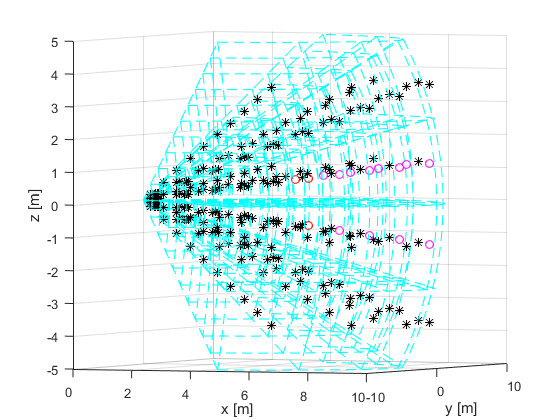
\includegraphics[width=0.6\linewidth]{\FIGDIR/38_Obstacle_assessment_phase.png}
    \caption{Obstacle assessment phase in avoidance grid.}
    \label{fig:gridObstacleAssessment}
\end{figure}

\noindent\textit{Reachability assessment} follows after obtaining pruned avoidance grid $\mathscr{A}(t_i)$. Because pruned avoidance grid $\mathscr{A}(t_i)$ already contains final reach set $\mathscr{R}(t_0,t_1,x_0)$ and hold \textit{trajectory belonging} property, one can say if there exist at least one trajectory $\mathscr{T}(x_0,B)$ to cell $c_{i,j,k}$, cell is reachable. Similar if there does not exist any trajectory $\mathscr{T}(x_0,B)$ to cell $c_{i,j,k}$, cell is unreachable. Reachability/Unreachability assessment is summarized in alg. \ref{alg:reachibilityAssessment}.
\\
\begin{algorithm}[H]
    \caption{Reachibility assessment}
    \label{alg:reachibilityAssessment}
    \SetKwInOut{Input}{Input}
    \SetKwInOut{Output}{Output}
    \Input{Pruned avoidance grid $\mathscr{A}(t_i)$.}
    \Output{Reachable avoidance grid $\mathscr{A}(t_i)$}
    \ForEach{Grid cell $c_{i,j,k}\in \mathscr{A}(t_i)$}{
        \If{$c_{i,j,k}$.status == 'Not determined'}{
            \If{$c_{i,j,k}$.trajectoriesCount()$\ge$ 1}{
                cell.status='Reachable'\;
            }\Else{cell.status='Unreachable'\;}
        }
        
    }
\end{algorithm}
\noindent\textit{Reachability assessment} example is displayed in figure \ref{fig:gridReachabilityAssessment}. Cell status is exact as in figure \ref{fig:gridObstacleAssessment}., cells with \textit{reachable} status are marked as green stars and cells with \textit{unreachable} state are marked as red crosses

\begin{figure}[H]
    \centering
    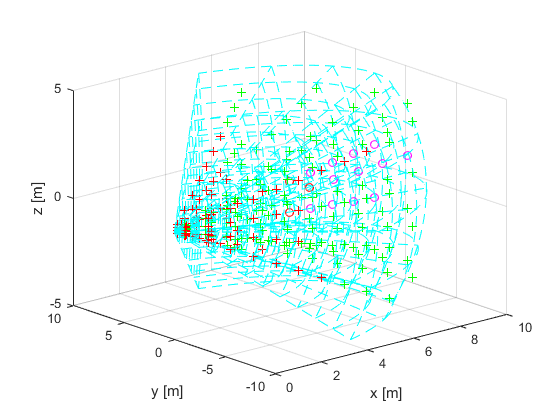
\includegraphics[width=0.6\linewidth]{\FIGDIR/40_Unreachability_assesment_phase.png}
    \caption{Reachibility assessment in avoidance grid.}
    \label{fig:gridReachabilityAssessment}
\end{figure}


\subsection{Avoidance goal selection}\label{ch:avoidanceGoalSimlistic}
\noindent The reachable space $\mathscr{R}$ in avoidance space $\mathscr{A}$ have been estimated. There comes decision where vehicle should fly and which control input should be used to bring vehicle to this point. For theoretical purposes decision making process under uncertainty is omitted. Main purpose of this section is to obtain \textit{avoidance goal} $c_{i,j,k}$ and control input $u(t+t+i)$. Because vehicle is controlled trough movement automaton $\textit{MA}$, movement buffer $B$ will be sufficient for control purposes. Movement automaton $\mathscr{MA}$ can translate movement buffer $B$ to desired control input $u(t+t_i)$.
Let define goal waypoint $\mathscr{WP}$ with global coordinates $[x_g,y_g,z_g]$ and local coordinates $[x_l,\theta_l,\varphi_l]$ in avoidance grid $\mathscr{A}$ coordinate frame. There exist distance function $f(\mathscr{WP},c_{i,j,k})$ which returns euclidean distance between waypoint $\mathscr{WP}$ and center of cell $c_{i,j,k}$. Minimal distance is selection criterion for goal cell $c_{i,j,k}$. Similarly each trajectory $\mathscr{T}(x_0,B)$ belonging to cell $c_{i,j,k}$ have cost $J^*(x,u)$, therefore trajectory movement buffer $B$ for trajectory with minimal cost is selected. Selection process for this simplistic case is summarized in alg. \ref{alg:goalSelectionExample}.  
\begin{algorithm}[H]
    \caption{Example of avoidance goal selection.}
    \label{alg:goalSelectionExample}
    \SetKwInOut{Input}{Input}
    \SetKwInOut{Output}{Output}
    \Input{Avoidance grid $\mathscr{G}_{3D}$, Goal waypoint $\mathscr{WP}_{g}$}
    \Output{Avoidance goal cell $c_{i,j,k}\in\mathscr{A}(t_i)$, Avoidance movement buffer $B$}
    minimalDistance = $\infty$\;
    \ForEach{$c_{i,j,k}\in\mathscr{A}(t_i)$ where $c_{i,j,k}$.status == 'Reachable'}{
        \If{distance($c_{i,j,k},\mathscr{WP}_{g}$) $<$ minimalDistance)}{
            minimalDistance =  distance($c_{i,j,k},\mathscr{WP}_{g}$)\;
            goalCell = $c_{i,j,k}$\;
        }
    }
    minimalCost = $\infty$
    \ForEach{$\mathscr{T}(x_0,B)\in$goalCell}{
        \If{$\mathscr{T}(x_0,B)$.cost $<$ minimalCost}{
            minimalCost =  $\mathscr{T}(x_0,B)$.cost\;
            movementBuffer = $\mathscr{T}(x_0,B)$.buffer\;
        }
    }
    \Return{[goalCell,movementBuffer]}\;
\end{algorithm}

\subsection{Avoidance execution}
\noindent\textit{Avoidance execution} shows reach set estimation method in context of control implementation. Given system $\dot{x}=f(x,u)$ with movement automaton $\mathscr{MA}$ control is controlled via movement buffer $B$, which contains ordered set of movements $\left\{m_1(t_1),\dots,m_j(t_j)\right\}$. Vehicle is equipped with sensor system which have visibility grid $\mathscr{G}_{3D}$. This visibility grid have pre-calculated maximal reach set $\mathscr{R}_0(t_0,t_1,x_0)$ defined by def. \ref{def:NumericReachSet3D}. Visibility grid $\mathscr{G}_{3D}$ and maximal reach set $\mathscr{R}_0(t_0,t_1,x_0)$ are fused into avoidance grid $\mathscr{A}(t_i)$ as defined in section \ref{ch:estimatedReachSetMethod}. Goal for avoidance is determined as described in section \ref{ch:avoidanceGoalSimlistic}. 

Let say vehicle should execute mission plan given by set of waypoints $\left\{\mathscr{WP}_1,\dots,\mathscr{WP}_{n}\right\}$. Movement automaton $\mathscr{MA} $buffer $B$ is flush-able, therefore new ordered set of movements can be inserted after currently processed movement. Avoidance execution is summarized in alg. \ref{alg:avoidanceFramework}. Main cycle is selecting waypoint to reach $\mathscr{WP}$, while inner cycle executes avoidance operation to prevent vehicle collision. Avoidance time $t_i$ is predicted, this time is given as time of last planned movement execution. Empty avoidance grid $\mathscr{A}(t_i)$ for predicted vehicle state $x(t_i)$ is loaded. From visibility grid all augmented obstacles $[d_o,\theta_o,\varphi_o]\in\mathscr{O}$ are put into the avoidance grid (alg. \ref{alg:06}.). Then avoidance goal $c_{i,j,k}$ cell and movement buffer $B$ are selected (alg. \ref{alg:goalSelectionExample}.). Maneuvers obtained from avoidance trajectory $\mathscr{T}(x(t_i),B)$ are inserted into movement automaton $\mathscr{MA}$ execution queue. When vehicle reaches avoidance time $t_i$, movement automaton starts to execute movements $m_j(t_j)\in B$. Defined count of movements is executed in parallel to next avoidance grid $\mathscr{A}(t_{i+1})$ processing. Inner cycle repeats until goal waypoint $\mathscr{WP}_n$ is reached.
\\
\begin{algorithm}[H]
    \label{alg:avoidanceFramework}
    \caption{Obstacle avoidance execution}
    \SetKwInOut{Input}{Input}
    \Input{Mission plan $\left\{\mathscr{WP}_1,\dots,\mathscr{WP}_{n}\right\}$,\\ Plain avoidance grid $\mathscr{A}(t_i),$\\
    Controlled vehicle with $\mathscr{MA}$ control,\\
    Count of executed movements $count$}
    \ForEach{waypoint $\mathscr{WP}_i$ in mission plan}{
    \While{!isWaypointReached($\mathscr{WP}_i$)}{
        $t_i$ = calculateAvoidanceTime($\mathscr{MA}$)\;
        $\mathscr{A}(t_i)$ = loadEmpty$\mathscr{A}(t_i)$()\;
        \ForEach{point $[x_o,\theta_o,\varphi_o]$ in $\mathscr{O}$}{
            putObstacle($\mathscr{A}(t_i)$,$[d_o,\theta_o,\varphi_o]$)(alg. \ref{alg:06}.)\;
            }
        [cell,buffer] = goalSelection($\mathscr{G}_{3D}$,$\mathscr{WP}_i$)(alg. \ref{alg:goalSelectionExample}.)\;
        setMovementBuffer($\mathscr{MA}$,buffer)\;
        executionMovements = getMovements($\mathscr{MA}$,count)\;
        \While{movement $m_j(t_j)\in$executionMovements}{
            $\mathscr{MA}$.executeMovement($m_j$,$t_j$)\;
        }
        }
    }
\end{algorithm}
Proposed avoidance execution with suitable window of opportunity guarantees avoidance of obstacles in environment holding assumptions \ref{ass:1},\ref{ass:3},\ref{ass:4},\ref{ass:5},\ref{ass:6},\ref{ass:7},\ref{ass:8}.
\chapter{Simulation results}\label{ch:simulationResults}

\section{Playground definition}\label{ch:3DPlaygroundDefinition}
\noindent For purpose of testing, new playground (\ref{fig:new3DPlayground})with added dimension needs to be introduced. Additional element of \textit{mission control} needs to be introduced, because previous experiments was with not coordinated flight and for real missions some coordinated flight is required, therefore waypoint set $\mathscr{WP}$ is added into playground. 
\begin{figure}[H]
    \centering
    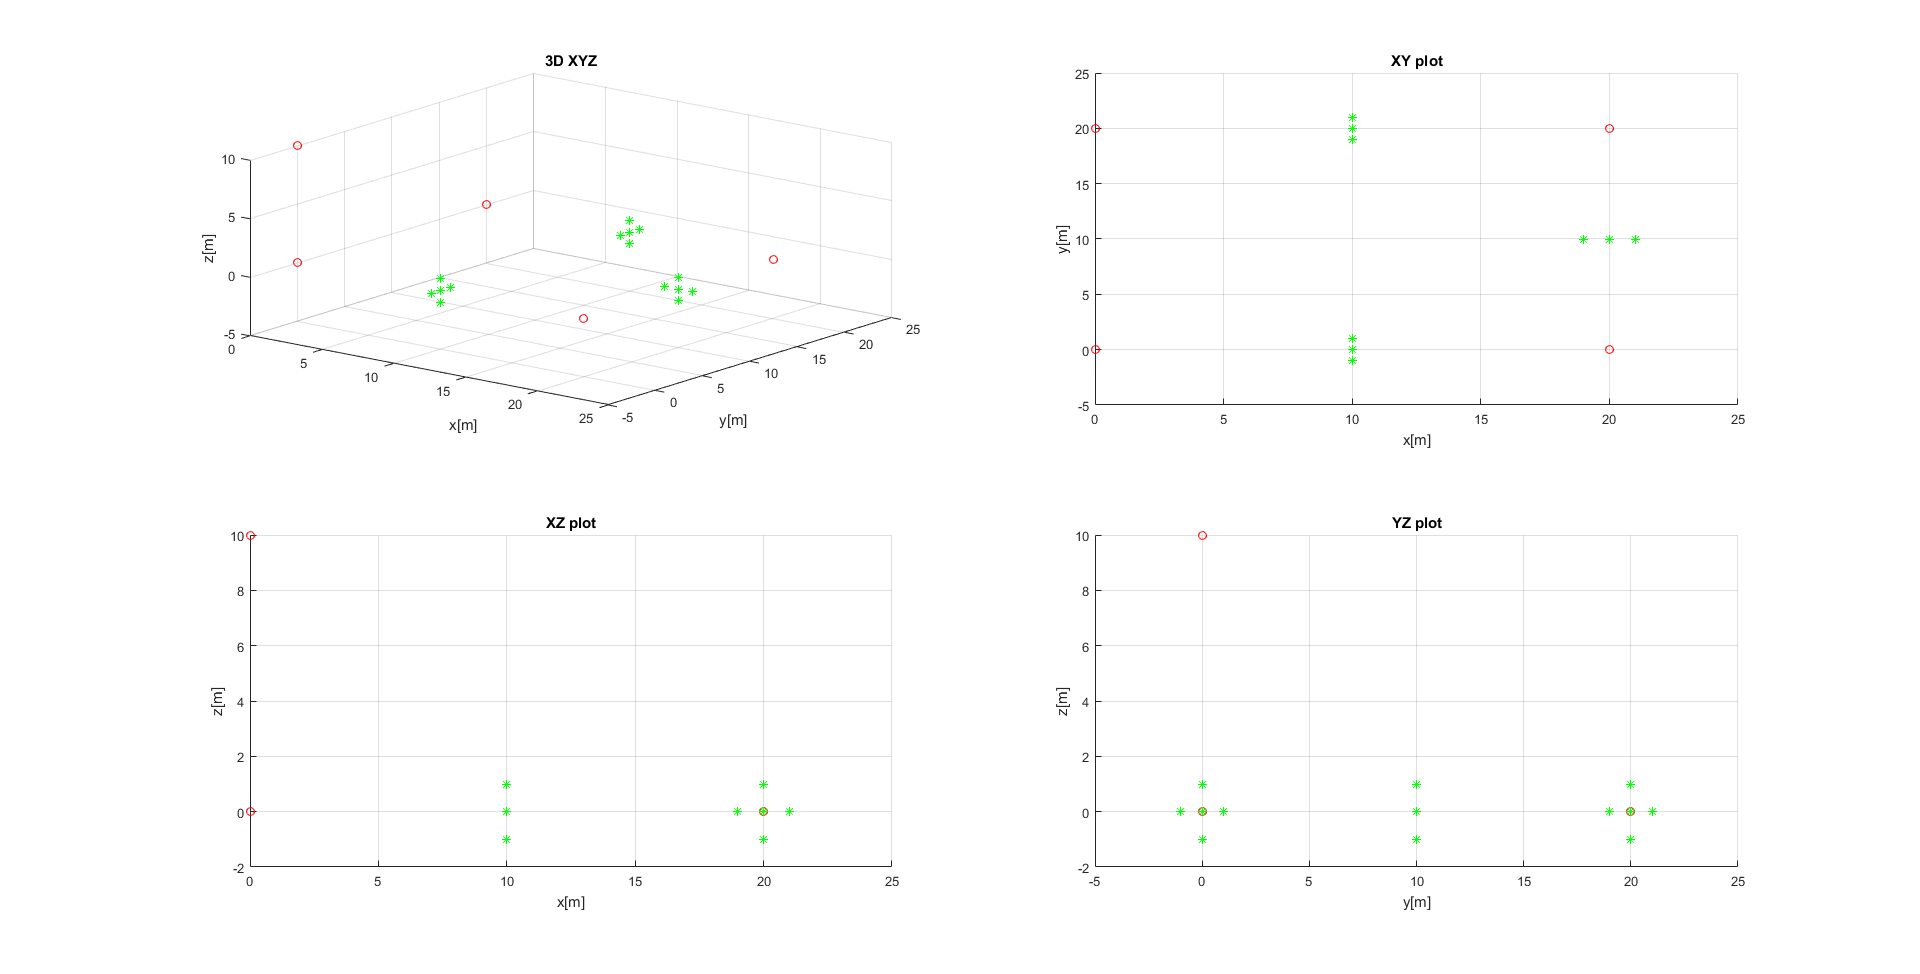
\includegraphics[width=\linewidth]{\FIGDIR/37_Playground_3D.png}
    \caption{Initial playground for obstacle avoidance and optimal path finding testing}
    \label{fig:new3DPlayground}
\end{figure}
\noindent Waypoint set $\mathscr{WP}$ (\ref{eq:playground3DSimpleWPSet}) contains five waypoins in Cartesian coordinates $\mathscr{WP}_i =[x,y,z]^T$. This set is simple rectangular flight around rectangle with side of 20 meters and slightly elevated end by 10 meters $\mathscr{WP}_E$.

\begin{equation}\label{eq:playground3DSimpleWPSet}
    \begin{aligned}
          \mathscr{WP} = \{ \mathscr{WP}_S &=[0,0,0]^T,\\
                            \mathscr{WP}_1 &=[20,0,0]^T,
                            \mathscr{WP}_2 =[20,20,0]^T,\\
                            \mathscr{WP}_3 &=[0,20,0]^T,
                            \mathscr{WP}_E =[0,0,10]^T,\}
    \end{aligned}
\end{equation}
\newpage 
\noindent Each path tracking algorithm needs to have stop condition which indicates when vehicle should stop following presented waypoint. Usually unit ball stop condition is used (\ref{eq:stopFunctionUnitBall}) where $[x_v,y_v,z_v]^t$ is vehicle position, $[x_g,y_g,z_g]^T$ is waypoint position and $p_t$ is precision threshold.
\begin{equation}\label{eq:stopFunctionUnitBall}
    \norm{\begin{bmatrix}x_g-x_v\\y_g-y_v\\z_g-z_v\end{bmatrix}} \le p_t
\end{equation}
Single obstacle $o_i\in\mathscr{O}$ is defined by its position $o=[x_o,y_o,z_o]^T$. All obstacles are stored in single obstacle structure $\mathscr{O}$ defined by (\ref{eq:3dSimplisticPlaygroundO}).
\begin{equation}\label{eq:3dSimplisticPlaygroundO}
    \mathscr{O} = \{\mathscr{O}_1,\mathscr{O}_2,\mathscr{O}_3\}
\end{equation}
Obstacle subset $\mathscr{O}_1$ (\ref{eq:3dSimplisticPlaygroundO1}) is defined between waypoints $\mathscr{WP}_S,\mathscr{WP}_1$.
\begin{equation}\label{eq:3dSimplisticPlaygroundO1}
    \mathscr{O}_1 = \{[10,0,0]^T,[10,1,0]^T,[10,-1,0]^T,[10,0,1]^T,[10,0,-1]^T\}
\end{equation}
Obstacle subset $\mathscr{O}_2$ (\ref{eq:3dSimplisticPlaygroundO2}) is defined between waypoints $\mathscr{WP}_1,\mathscr{WP}_2$.
\begin{equation}\label{eq:3dSimplisticPlaygroundO2}
    \mathscr{O}_2 = \{[20,10,0]^T,[20,10,1]^T,[20,10,-1]^T,[19,10,0]^T,[21,10,0]^T\}
\end{equation}
Obstacle subset $\mathscr{O}_3$ (\ref{eq:3dSimplisticPlaygroundO3}) is defined between waypoints $\mathscr{WP}_2,\mathscr{WP}_3$.
\begin{equation}\label{eq:3dSimplisticPlaygroundO3}
    \mathscr{O}_3 = \{[10,20,0]^T,[10,20,1]^T,[10,20,-1]^T,[10,19,0]^T,[10,21,0]^T\}
\end{equation}

\section{Movement automaton predictor}\label{ch:movementAutomatonPredictor}
\noindent Vehicle system is given by model from section \ref{sec:3DsimplisticplaneModel}. Vehicle control is defined as movement automation $\mathscr{MA}$ with rapid exploration movement set defined in equation \ref{eq:rapidExplorationMovementSet}. Movement predictor needs to be developed in order to obtain control signal $u(t)$ It is possible to predict movement buffer $B_{\mathscr{MA}}$, between vehicle initial position $x_0$ and waypoint, when known obstacle set $\mathscr{O}$ is given and movement state can be predicted for chain of movements. This approach have been defined in alg. \ref{alg:05}. as rapid exploration tree. 

Vehicle state $x(t_0)$ at start of mission execution is known. Vehicle state in discrete time $x(t)$ is given by equation \ref{eq:vehicleStateDiscreteKnown}. Where $x_v(t),y_v(t),z_v(t)$ is vehicle position in local coordinate frame and $\alpha_v(t),\beta_v(t),\gamma_v(t)$ is vehicle orientation angles.
\begin{equation}\label{eq:vehicleStateDiscreteKnown}
    x(t) = [x_v(t),y_v(t),z_v(t),\alpha_v(t),\beta_v(t),\gamma_v(t)]^T;
\end{equation}
Base movement table for movements $m_i(1)\in M$ have been measured on system model (\ref{sec:3DsimplisticplaneModel}). This table represents vehicle position and orientation differences after execution of movement. Vehicle initial state was set at center of local coordinate frame with narrow orientation $[x_0,y_0,z_0]=[0,0,0]$. Vehicle initial orientation was aligned with main frame axis X, therefore initial orientation angles are $[\alpha_0,\beta_0,\gamma_0] = [0,0,0]$. Vehicle velocity was set to constant value $v_v = 1 ms^{-1}$. Vehicle position after movement execution is given by parameters $x_b,y_b,z_b$ at time $t+1$. Vehicle orientation is given by parameters $\alpha_b,\beta_b,\gamma_b$. Givem parameters are also absolute shifting, because initial state is $[x_0,y_0,z_0,\alpha_b,\beta_b,\gamma_b]$ set to $\vec{0}$.
\begin{table}[H]
    \centering
    \begin{tabular}{|l||c|c|c|c|c|}
    \hline
        $v_x/m_i$           &    Straight $\circledcirc$ & Down $\Downarrow$  & Up $\Uparrow$    & Left $\Leftarrow$ & Right $\Rightarrow$\\\hline\hline
        $x_b [m]$           &    1.00	  & 0.98  & 0.98  & 0.98 & 0.98\\\hline
        $y_b [m]$           &    0	      & 0	  & 0	  & 0.13 & -0.13\\\hline
        $z_b [m]$           &    0	      & -0.13 & 0.13  &	0	 & 0\\\hline
        $\alpha_b [rad]$	&    0	      & 0	  & 0	  & 0    & 0\\\hline
        $\beta_b [rad]$     &    0	      & 0.2   & -0.26 & 0	 & 0\\\hline
        $\gamma_b [rad]$    &    0	      & 0	  & 0	  & 0.26 & -0.26\\\hline
    \end{tabular}
    \caption{Base values for movement application, vehicle position difference $x_v,y_v,z_v$ and orientation differences $\alpha_v,\beta_v,\gamma_v$.}
    \label{tab:movementPredictor}
\end{table}
\noindent With defined base movement table (tab. \ref{tab:movementPredictor}). with defined shifting for movement at time $t_0+1$, \textit{rotation} (\ref{eq:rotationSimplisticPredictor}) and \textit{shifting} (\ref{eq:shiftingSimplisticPredictor}) equations must be defined in order to obtain predicted position $\hat{x}(t+1)$. Position after movement execution $[\hat{x}(t+1),\hat{y}(t+1),\hat{z}(t+1)]$ is depending on vehicle orientation before movement execution $[\alpha_v(t),\beta_v(t),\gamma_v(t)]$. Rotation function rotates vehicle position $[x_b(t_0),y_b(t_0),z_b(t_0)]$ according to vehicle orientation angles $[\alpha_v(t),\beta_v(t),\gamma_v(t)]$. For rotation standard rotation matrix $R_{XYZ}(\alpha,\beta\gamma)$ (\ref{eq:xyzspaceRotationMatrix}) is used. Final position offset vector $[\tilde{x}_b(t+1),\tilde{y}_b(t+1),\tilde{z}_b(t+1)]$ at predicted time $t+1$ is given by equation \ref{eq:rotationSimplisticPredictor}.
\begin{equation}\label{eq:rotationSimplisticPredictor}
    \begin{bmatrix}
        \tilde{x}_b\\ 
        \tilde{y}_b\\
        \tilde{z}_b\\
    \end{bmatrix}
    = R_{XYZ}(\alpha_v(t),\beta_v(t),\gamma_v(t))
    \begin{bmatrix}
        x_b\\ 
        y_b\\
        z_b\\
    \end{bmatrix}
\end{equation}
Predicted state vector $\hat{x}(t+1)$ a at time $t+1$ is obtained by combining position offset vector $[\tilde{x}_b(t+1),\tilde{y}_b(t+1),\tilde{z}_b(t+1)]$, orientation offset vector $\alpha_b(t+1),\beta_b(t+1),\gamma_b(t+1)$. as given in equation \ref{eq:shiftingSimplisticPredictor}.\\
\begin{equation}\label{eq:shiftingSimplisticPredictor}
    \begin{aligned}
    \hat{x}(t+1) & = [\hat{x}_v(t+1),\hat{y}_v(t+1),\hat{z}_v(t+1),\hat{\alpha}_v(t+1),\hat{\beta}_v(t),\hat{\gamma}_v(t)]^T\\
    \hat{x}_v(t+1) & = x_v(t)+\tilde{x}_b\\
    \hat{y}_v(t+1) & = y_v(t)+\tilde{y}_b\\
    \hat{z}_v(t+1) & = z_v(t)+\tilde{z}_b\\
    \hat{\alpha}_v(t+1) & = \alpha_v(t) + \alpha_b\\
    \hat{\beta}_v(t+1) & = \beta_v(t) + \beta_b\\
    \hat{\gamma}_v(t+1) & = \gamma_v(t) + \gamma_b
    \end{aligned}
\end{equation}
Movement automaton $\mathscr{MA}$ has chaining property, therefore movement prediction chaining is also possible via recursive procedure for discrete execution time $t_i$. There exist predicted movement buffer $\hat{B}$ with ordered movement sequence $m_1(1),\dots,m_i(1)$, vehicle state after applying movement $m_{i+1}$ at time $t_i$ can be obtained via equation \ref{eq:discretePredictionChaining}.
\begin{equation}\label{eq:discretePredictionChaining}
    \hat{x}(t_i+1) = f(\hat{x}(t_i),m_{i+1}(1))
\end{equation}
Prediction function $f(\hat{x}(t_i),m_{i+1}(1))$ is in this case function defined by equation \ref{eq:shiftingSimplisticPredictor}, where parameters $[x_b,y_b,z_b,\alpha_b,\beta_b\gamma_b]$ are selected based on movement $m_{i+1}(1)$ type from lookup table  \ref{tab:movementPredictor}.


\section{Obstacle avoidance in partially known environment}
\noindent Obstacle avoidance is different in partially known environment, because uncertainty plays great role in control and decision making. Future obstacle avoidance theorem will be developed. Avoidance implementation have been verified at playground defined in section \ref{ch:3DPlaygroundDefinition}. Known world $\mathscr{F}$ have been mentioned multiple times over thesis. In case of reactive obstacle avoidance it is necessary to acknowledge that know world $\mathscr{F}$ is equal to $\mathscr{G}_{3D}$. Most of the time visible space (def. \ref{def:VisibleSpace}) is equal to visibility grid (def. \ref{def:visibilityGridCell}). Let say that for each discrete scanning time $t_i$ there exist avoidance grid $\mathscr{A}(t_i)$ which is valid for time $t\in[t_i,t_i+\tau)$, where $\tau$ is life time of scanned data. In real situation is frame life time $\tau$ equal to some finite time, acquired trough experience with sensor and flight environment. In this testing case $\tau = \infty$, because experience with chosen sensor and environment are not known now.
Known world $\mathscr{F}$ at time $t\ge t_0$ in this scenario is given by following equation:
\begin{equation}
    \mathscr{F}(t) = \left\{\vec{p}\in \R^3: \exists\mathscr{F}_{3D}(t_i),t_0\le t_i \le t, \vec{p} \in \mathscr{g}_{3D}(t_i) \right\}
\end{equation}
Known world at the end of simulation is displayed in following figure \ref{fig:visibleVsReachableLocalFrame}.
\begin{figure}[H]
    \centering
    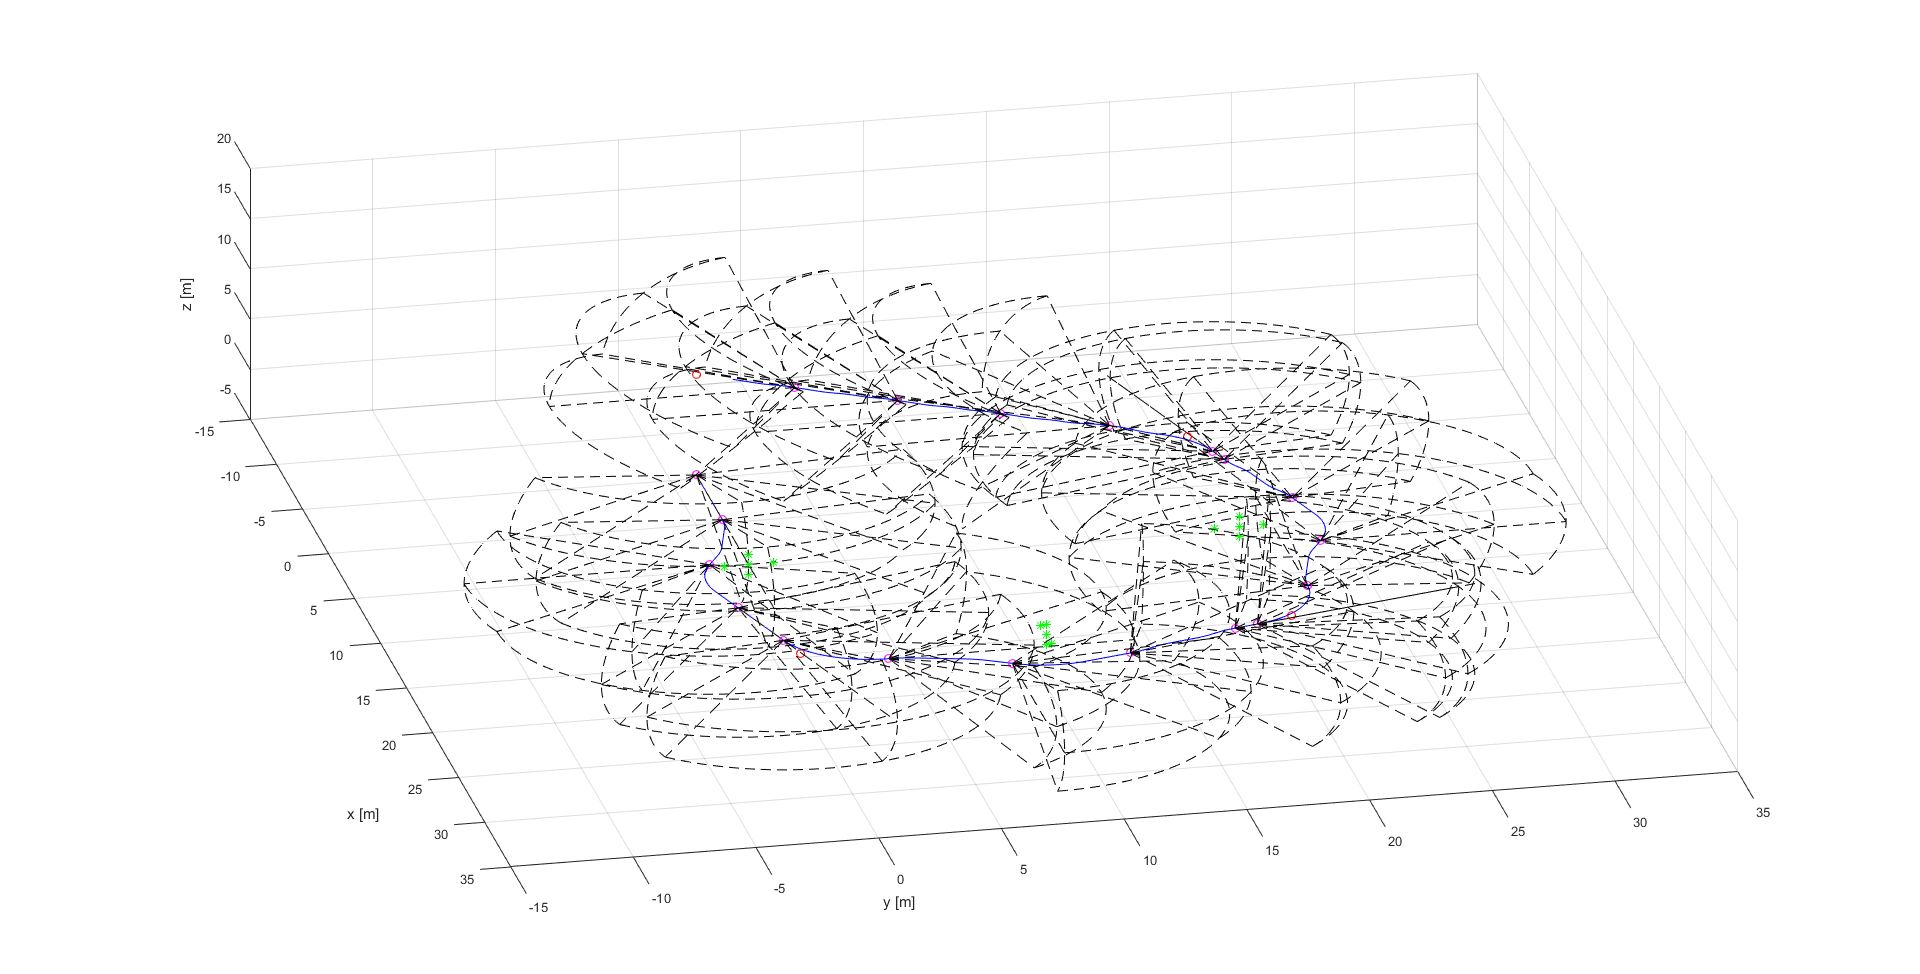
\includegraphics[width=\linewidth]{\FIGDIR/42_Known_world_during_flight.png}
    \caption{Known world during flight in virtual playground.}
    \label{fig:knownWorldDuringFlight}
\end{figure}

\noindent For testing purposes simple cost function $J^*(x(t_i),\mathscr{MA}(t_i))$ is defined for pre-calculated maximal reach set $\mathscr{R}(t_0,t_1,x_0)$ given by def. \ref{def:NumericReachSet3D}. Cost function $J^*$ (\ref{eq:simpleCostFunctionReachSetTest}) is calculated for discrete avoidance time $t_i$ as Euclidean position difference for vehicle position $[x_v,y_v,z_v]$ with penalisation coefficient $c_p(m_k)$ (\ref{eq:penalisationCoeficientSimple}).
\begin{equation}\label{eq:simpleCostFunctionReachSetTest}
    J^*(x(t_i),\mathscr{MA}(t_i) = \sum_{k=1}^i \left(\sqrt{ 
    \begin{aligned}
    &\left(x_v(t_k)-x_v(t_{k-1})\right)^2\\
    +&\left(y_v(t_k)-y_v(t_{k-1})\right)^2\\
    +&\left(z_v(t_k)+z_v(t_{k-1})\right)^2 
    \end{aligned}}\right)c_p(m_k) 
\end{equation}
Purpose of penalisation coefficient $c_p(m_k)$ (\ref{eq:penalisationCoeficientSimple}) is to prefer movements in order: straight($\circledcirc$), right($\Rightarrow$), left($\Leftarrow$), up($\Uparrow$) and down($\Downarrow$). For each trajectory $\mathscr{T}(x_0,B)$ passing trough goal cell $c_{i,j,k}$ cost $J^*$ is assigned, therefore goal determination algorithm (alg. \ref{alg:goalSelectionExample}.) can select best avoidance trajectory $\mathscr{T}(x_0,B)$ in avoidance framework inner cycle (alg. \ref{alg:avoidanceFramework}).
\begin{equation}\label{eq:penalisationCoeficientSimple}
    c_p(m_k)=
    \begin{cases}
        1 :&\text{if} m_k =\circledcirc \\
        1.5 :&\text{if} m_k = \Leftarrow\text{ or }m_k = \Rightarrow\\
        2 :\text{if}& m_k = \Uparrow\text{ or }m_k = \Downarrow
    \end{cases}
\end{equation}
Let say that testing vehicle is occupying in unit-ball $\mathscr{B}$ with diameter $0.30$ m, therefore minimal safety margin is $s_m=0.3m$. Turning radius of vehicle is $2$ meters. If potentional field method is used \cite{koren1991potential}. Minimal safety margin $s_m$ of  $2.6$ meters will be used. Presented obstacle avoidance framework can potentially reduce safety margin $s_m$ to diameter of vehicle unit ball $\mathscr{B}$ and predicted trajectory error $e_p$. Because prediction error $e_p$ have been measured in worst case scenario as $0.3$ meters, therefore safety margin $s_m$ is set as $0.6$ meters. 

Standard LiDAR sensor can scan up to $200$ meters in front of the vehicle. Let us assume very bad weather conditions. According to case study \cite{ramasamy2016lidar} worst possible visibility range in fog with heavy rain is $10$ meters. Using these parameters testing visibility grid is defined as equation \ref{eq:FOVsim3D}.
\begin{equation}\label{eq:FOVsim3D}
    \mathscr{G}_{3D}(d_s=0m,d_e=10m,\theta_s = \frac{\pi}{3},\theta_e =-\frac{\pi}{3},\varphi_s =\frac{pi}{6},\varphi_e=-\frac{pi}{6}).     
\end{equation}


\noindent Movement automaton $\mathscr{MA}$ buffer $B_{\mathscr{MA}}$ is filled with 1 to 10 movements based on actual avoidance grid $\mathscr{A}(t_i)$. at time of avoidance execution $t_i$. Obstacle avoidance algorithm is executed every time when vehicle moves half of visibility grid (every $\sim$5 s). When avoidance algorithm finishes ($\sim$ 0.5 s) movement automaton buffer $B_{\mathscr{MA}}$ is flushed and previously planned movements are replaced with new ones.

Two separate cases are considered to verify aspects of avoidance framework given by alg. \ref{alg:avoidanceFramework}.:
\begin{enumerate}
    \item \textit{Simple obstacle avoidance} - vehicle flies between two waypoints and encounters obstacles, this case shows decision making of obstacle avoidance framework.
    \item \textit{Mission plan execution} - vehicle executes mission plan defined in section \ref{ch:3DPlaygroundDefinition}, this case is to show complex mission execution, and discuss overall framework performance.
\end{enumerate}

\subsection{Simple obstacle avoidance}
\noindent Avoidance decision time $t_d$ is important parameter, because it is definef visibility grid $\mathscr{G}_{3D}$ overlaps in known world $\mathscr{F}$. Every decision time $t_d$ obstacle avoidance framework (alg. \ref{alg:avoidanceFramework}) is executed. For purpose of this simulation Movement automaton structure (def. \ref{def:movementAutomaton}.) is extended for:
\begin{enumerate}
    \item \text{Executed buffer} $B_E\in M^i$ - purpose is to store executed movements in decision time $t_0+kt_{d+1},k\in\N^+$, movements are stored after next decision frame $\mathscr{D}(t_d+1)$is invoked.
    \item \text{Planned buffer} $B_P\in M^i$ - purpose is to store planned movements in decision time $t_0+kt_{d},k\in\N^+$., movements are stored when actual decision frame is invoked $\mathscr{D}(t_d)$.
\end{enumerate}
Decision frame $\mathscr{D}(t_d)$  is deployed every decision time $t_d$. Six decision frames were deployed during this simulation. Main purpose is to show how decision frame impacts planned and flew trajectory.


For simple obstacle avoidance mission plan is defined by waypoint set $\mathscr{WP}$ (\ref{eq:simpleObstacleMissionPG1}) and obstacle set $\mathscr{O}$ (\ref{eq:simpleObstacleMissionPG2}). There is two waypoints $\mathscr{WP_S}$ and $\mathscr{WP}_E$ with mutual distance $30m$.
\begin{equation}\label{eq:simpleObstacleMissionPG1}
    \mathscr{WP}=\left\{\mathscr{WP}_S,\mathscr{WP}_E\right\} = \left\{[0,0,0],[30,0,0]\right\}
\end{equation}
Two obstacle sets $\mathscr{O}_1$ and $\mathscr{O}_2$ are put between waypoints $\mathscr{WP_S}$ and $\mathscr{WP}_E$ (\ref{eq:simpleObstacleMissionPG1}). Its assured that vehicle without avoidance system will crash into obstacle set $\mathscr{O}$.
\begin{equation}\label{eq:simpleObstacleMissionPG2}
    \begin{aligned}
    \mathscr{O}   &= \left\{\mathscr{O}_1,\mathscr{O2}\right\}\\
    \mathscr{O}_1 &= \left\{[10,0,0],[10,1,0)[10,-1,0],[10,0,1],[10,0,-1]\right\}\\
    \mathscr{O}_2 &= \left\{[10,0,0],[10,1,0)[10,-1,0],[10,0,1],[10,0,-1]\right\}
    \end{aligned}
\end{equation}

\noindent Decision frame is invoked $t_d=5s$, mission given by wapypoints $\mathscr{WP}$ and  obstacles $\mathscr{O}$ had six decisions frames defined at decision time $t_d\in T_d = \left\{0, 5, 10, 15, 20, 25\right\}$. Decisions made in decision time set $T_d$ are discussed in following text

\begin{figure}[H]
    \centering
    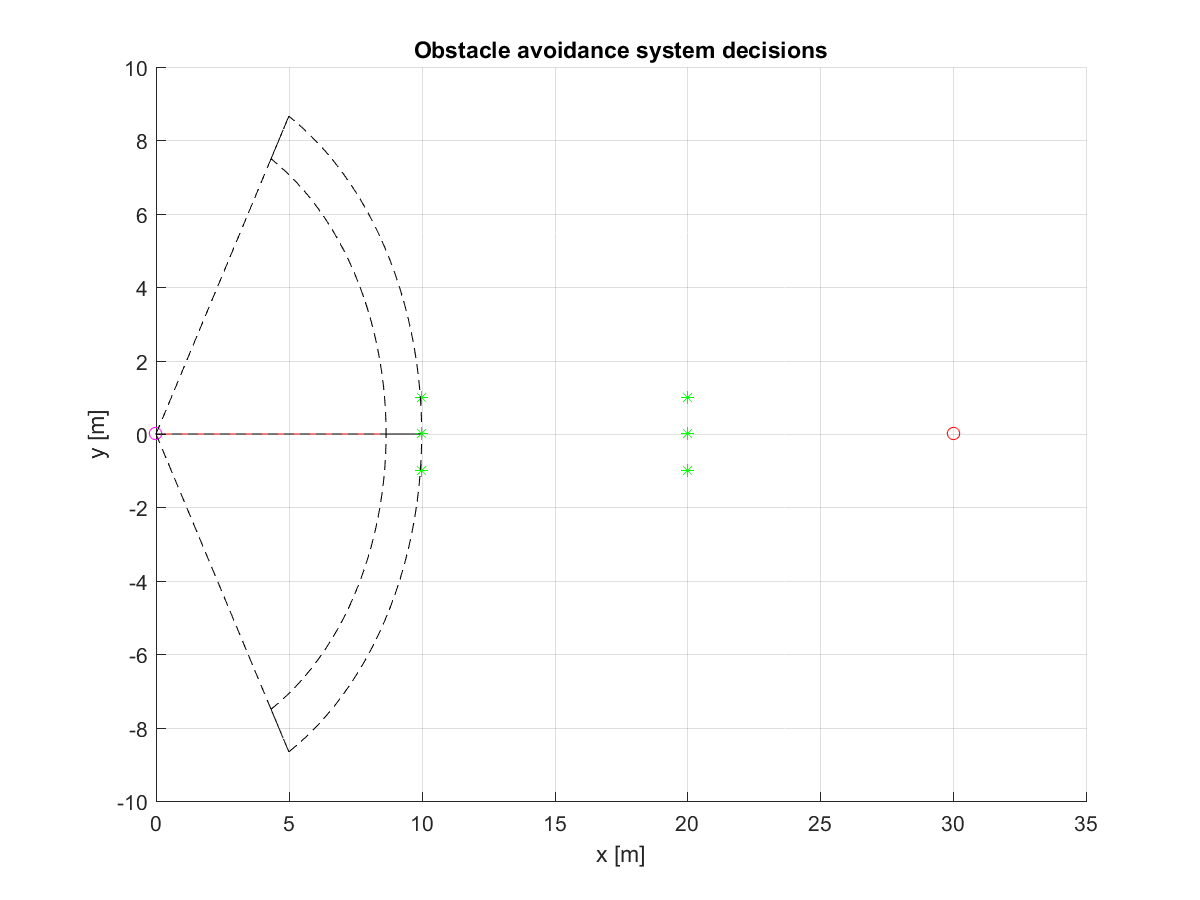
\includegraphics[width=0.7\linewidth]{\FIGDIR/64_AvoidanceFrame-01.png}
    \caption{Decision frame $\mathscr{D}(0)$.}
    \label{fig:decisionFrameSimple0}
\end{figure}
\noindent Decision $\mathscr{D}(0)$ is portrayed in figure \ref{fig:decisionFrameSimple0}. Vehicle is at initial position $x_0$ and visibility grid $\mathscr{G}_3D$ does not registered any approaching obstacle, therefore avoidance grid $\mathscr{A}(0)$ is identical to maximal avoidance grid. Goal cell $c_{i,j,k}$ is selected as closest cell to $\mathscr{WP}_E$. Planned movement buffer $B_P$ is filled with movement buffer from trajectory $\mathscr{T}(x_0,B)$. Five straight movement $\circledcirc(5)$ are executed as results. Without executing avoidance at decision time $t_d=5$ vehicle will surely crash to obstacle set $\mathscr{O}_1$.
Planned buffer $B_P$ for decision frame $\mathscr{D}(0)$ have following values $B_P$ = \textit{[$\mathscr{D}(0)$ $\circledcirc$(10)]}.
Executed buffer $B_E$ for decision frame $\mathscr{D}(0)$ have following values $B_P$ = \textit{[$\circledcirc$(5)]}.
\begin{figure}[H]
    \centering
    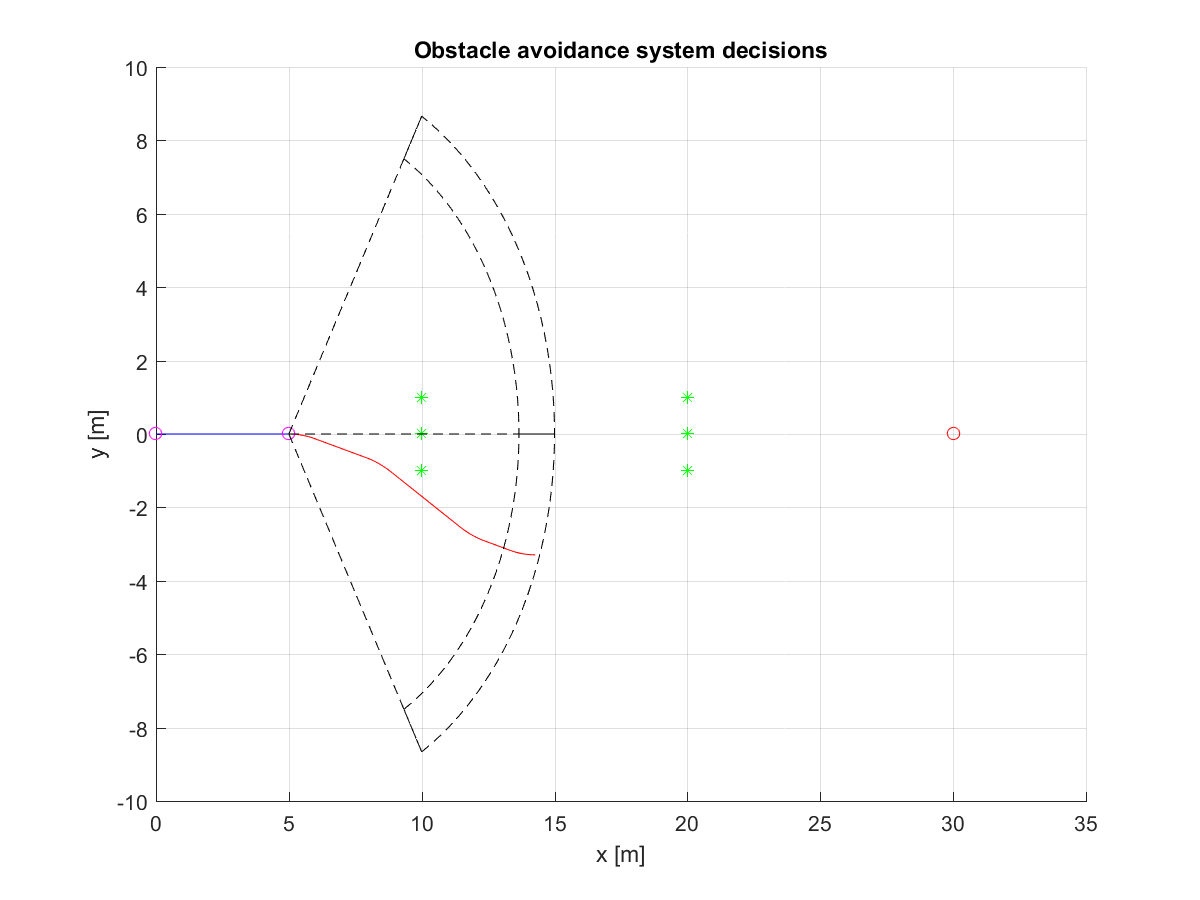
\includegraphics[width=0.7\linewidth]{\FIGDIR/65_AvoidanceFrame-02.png}
    \caption{Decision frame $\mathscr{D}(5)$.}
    \label{fig:decisionFrameSimple5}
\end{figure}
\newpage
\noindent Decision $\mathscr{D}(5)$ is portrayed in figure \ref{fig:decisionFrameSimple5}. Vehicle executed five of movements $m_i$ planned in decision frame $\mathscr{D}(0)$. Visibility grid $\mathscr{G}_{3D}$ is filled with obstacle set $\mathscr{O_1}$. Avoidance grid $\mathscr{A}(5)$ asses space inf front of the obstacle set $\mathscr{O}_1$ as \textit{'Uncertain'}, therefore any trajectory $\mathscr{T}(x_5,B)$ belonging to reduced reach set $\mathscr{R}(t_5,t_{10},x_{5})$ does not return to original course after passing an obstacle. Avoidance trajectory $\mathscr{A}(x_5,B)$ with lowest cost $J^*$ selected in goal cell $c_{i,j,k}$ closest to waypoint $\mathscr{WP}_E$. Avoidance priority is \text{straight, right, left, up and down}, because \text{straight} trajectory is not available \textit{right} avoidance trajectory is selected. Planed trajectory $\mathscr{T}(x_5,B_P)$ is deviating from original course, but is deemed as safe trajectory.
Planned buffer $B_P$ for decision frame $\mathscr{D}(5)$ have following values $B_P$ = \textit{[ $\Rightarrow$(1), $\circledcirc$(2), $\Rightarrow$(1), $\circledcirc$(3), $\Leftarrow$(1), $\Downarrow$(1), $\Leftarrow$(1)]}.
Executed buffer $B_E$ for decision frame $\mathscr{D}(5)$ have following values $B_P$ = \textit{[$\Rightarrow$(1), $\circledcirc$(2), $\Rightarrow$(1), $\circledcirc$(1)]}.     
\begin{figure}[H]
    \centering
    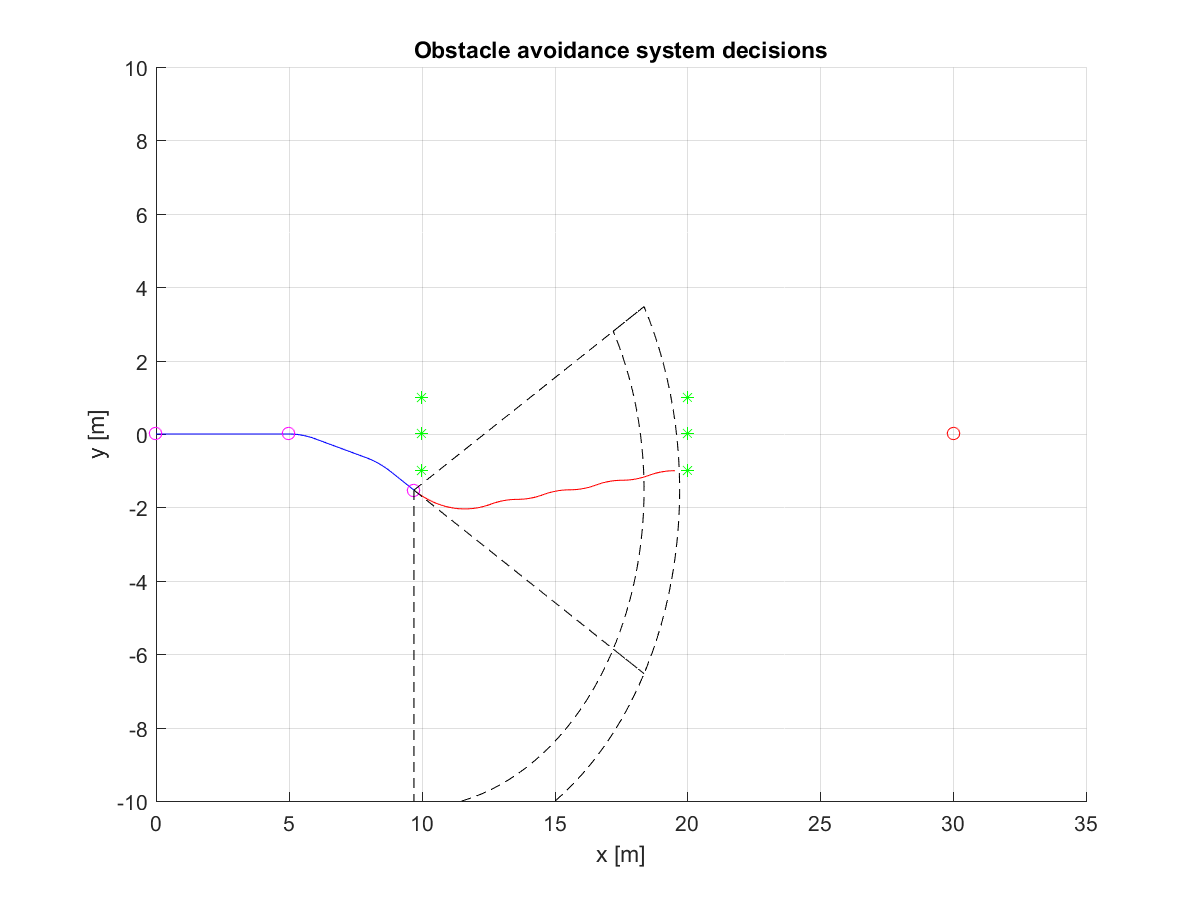
\includegraphics[width=0.7\linewidth]{\FIGDIR/66_AvoidanceFrame-03.png}
    \caption{Decision frame $\mathscr{D}(10)$.}
    \label{fig:decisionFrameSimple10}
\end{figure}
\noindent Decision $\mathscr{D}(10)$ is portrayed in figure \ref{fig:decisionFrameSimple10}. Vehicle executed five of movements $m_i$ planned in decision frame $\mathscr{D}(5)$. Visibility grid $\mathscr{G}_{3D}$. does not register obstacle set $\mathscr{O}_2$, because its behind border of vision. Avoidance grid $\mathscr{A}(t_{10})$ is loaded with maximal reach set $\mathscr{R}(t_{10},t_{15},x_{10})$. Goal cell $c_{i,j,k}$ with cheapest trajectory $\mathscr{T}(x_{10},B_P)$ is selected. At this state vehicle is planning to return to original trajectory between waypoints $\mathscr{WP}_S$ and $\mathscr{WP}_E$. If planned buffer $B_P$ was fulle executed at this state $x_{10}$, it will lead to crash at obstacle set $\mathscr{O}_2$.
Planned buffer $B_P$ for decision frame $\mathscr{D}(10)$ have following values $B_P$ = \textit{ [$\Leftarrow$(3), $\Rightarrow$(1), $\Leftarrow$(1), $\Rightarrow$(1), $\Leftarrow$(1), $\Rightarrow$(1), $\Leftarrow$(1), $\Rightarrow$(1)]}.
Executed buffer $B_E$ for decision frame $\mathscr{D}(10)$ have following values $B_P$ = \textit{[$\Leftarrow$(3), $\Rightarrow$(1), $\Leftarrow$(1]}.
\begin{figure}[H]
    \centering
    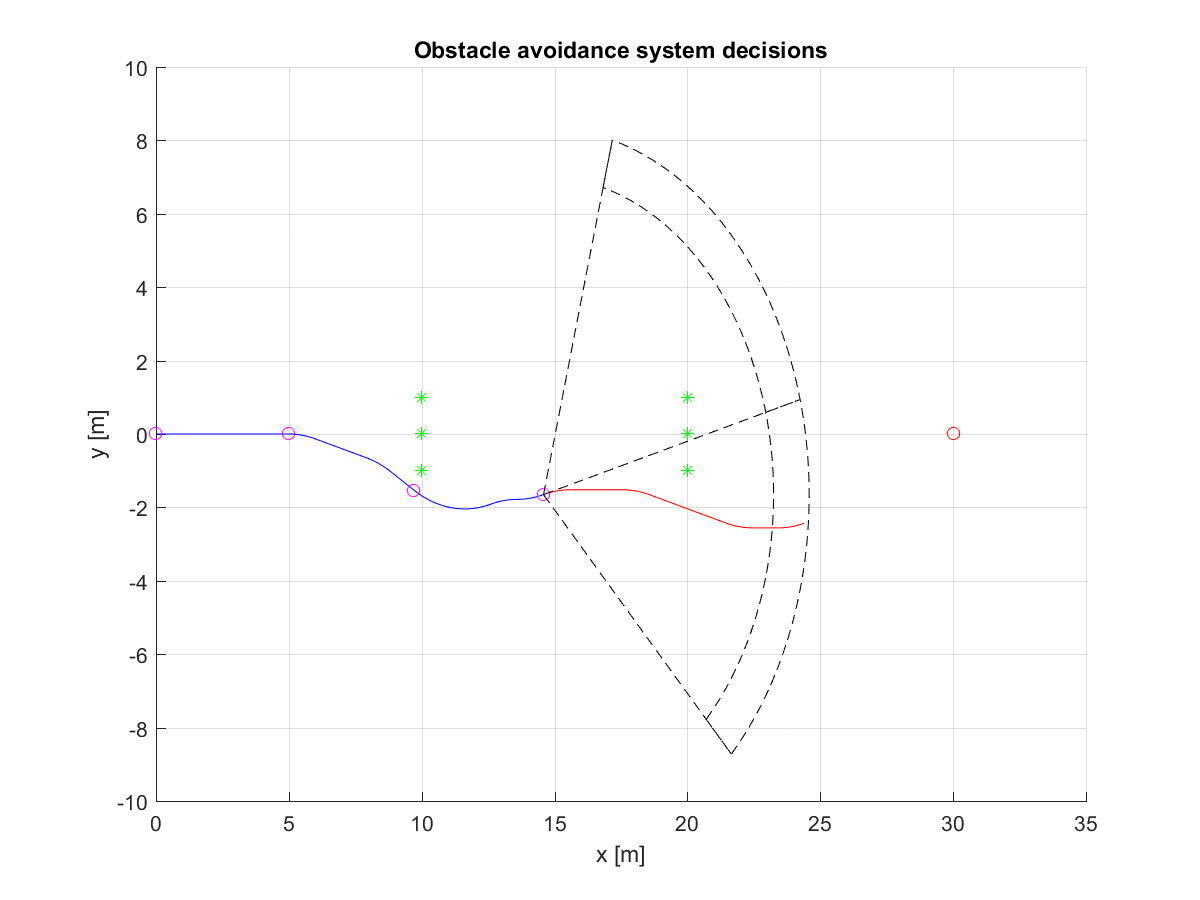
\includegraphics[width=0.7\linewidth]{\FIGDIR/67_AvoidanceFrame-04.png}
    \caption{Decision frame $\mathscr{D}(15)$.}
    \label{fig:decisionFrameSimple15}
\end{figure}
\noindent Decision $\mathscr{D}(15)$ is portrayed in figure \ref{fig:decisionFrameSimple15}. Vehicle executed five of movements $m_i$ planned in decision frame $\mathscr{D}(10)$. Visibility grid $\mathscr{G}_{3D}$ has detected obstacle set $\mathscr{O}_2$. Avoidance grid $\mathscr{A}(t_{15})$ is initialized and pruned, reduced reach set $\mathscr{R}(t_{15},t_{20},x_{15})$ is obtained. Goal cell $c_{i,j,k}$ closest to waypoint $\mathscr{WP}_E$ is selected. Trajectory $\mathscr{T}(x_{15},B_P)$ with lowest cost function $J*$ is selected as avoidance trajectory. Avoidance maneuver is avoiding detected obstacle set $\mathscr{O}_2$ from right side, due the avoidance maneuvers priority. 
Planned buffer $B_P$ for decision frame $\mathscr{D}(15)$ have following values $B_P$ = \textit{
[$\Rightarrow$(1), $\circledcirc$(2), $\Rightarrow$(1), $\circledcirc$(3), $\Leftarrow$(1), $\Downarrow$(1), $\Leftarrow$(1)]}.
Executed buffer $B_E$ for decision frame $\mathscr{D}(10)$ have following values $B_P$ = \textit{[$\Rightarrow$(1), $\circledcirc$(2), $\Rightarrow$(1), $\circledcirc$(1)]}.
\begin{figure}[H]
    \centering
    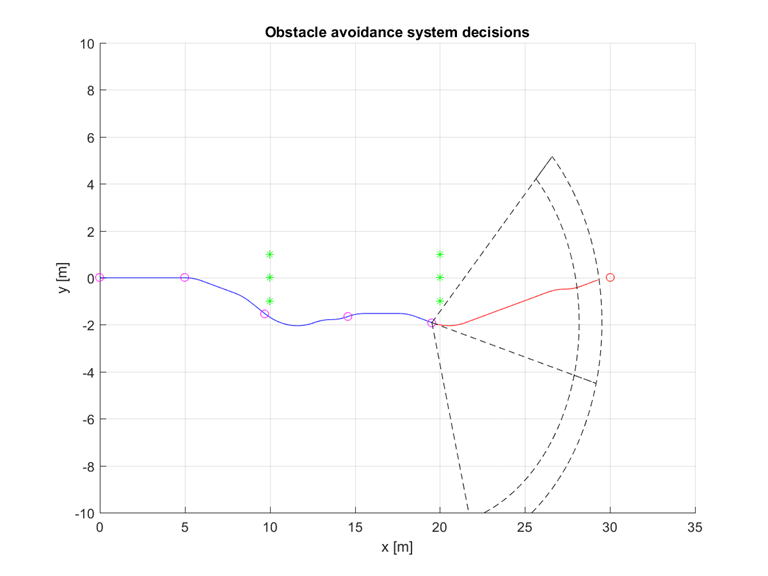
\includegraphics[width=0.7\linewidth]{\FIGDIR/68_AvoidanceFrame-05.png}
    \caption{Decision frame $\mathscr{D}(20)$.}
    \label{fig:decisionFrameSimple20}
\end{figure}
\noindent Decision $\mathscr{D}(20)$ is portrayed in figure \ref{fig:decisionFrameSimple20}. Vehicle executed five of movements $m_i$ planned in decision frame $\mathscr{D}(15)$. Visibility grid $\mathscr{G}_{3D}$ does not contain any obstacle, therefore shortest trajectory $\mathscr{T}(x_20,B_P)$ to $\mathscr{WP}_E$ is selected as avoidance trajectory. This decision is standard after avoidance decision and vehicle will return to original trajectory between $\mathscr{WP}_S$ and $\mathscr{WP}_E$.
Planned buffer $B_P$ for decision frame $\mathscr{D}(20)$ have following values $B_P$ = \textit{[$\Leftarrow$(2), $\circledcirc$(5), $\Rightarrow$(1), $\Leftarrow$(1), $\circledcirc$(1)]}.
Executed buffer $B_E$ for decision frame $\mathscr{D}(20)$ have following values $B_P$ =\textit{[$\Leftarrow$(2), $\circledcirc$(3)]}.
\begin{figure}[H]
    \centering
    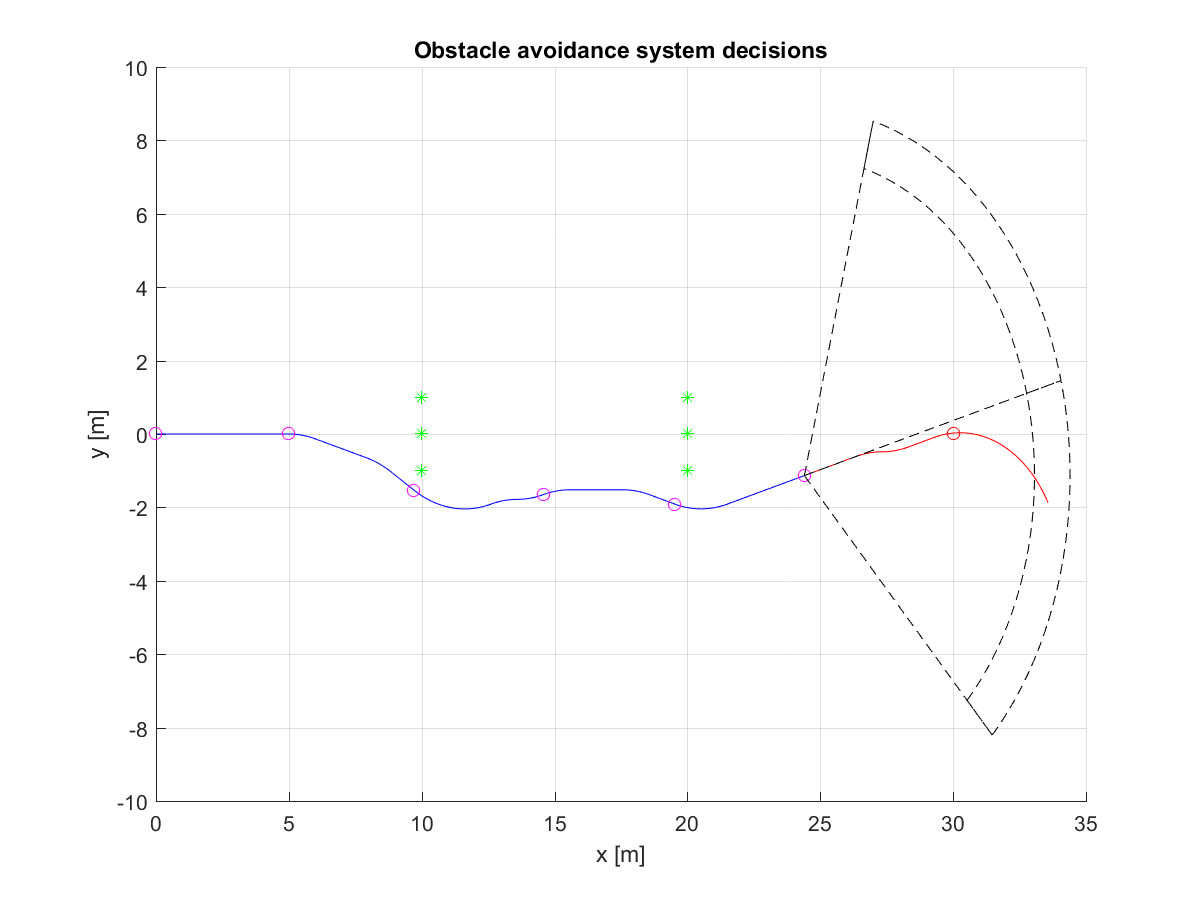
\includegraphics[width=0.7\linewidth]{\FIGDIR/69_AvoidanceFrame-06.png}
    \caption{Decision frame $\mathscr{D}(25)$.}
    \label{fig:decisionFrameSimple25}
\end{figure}
\noindent Decision $\mathscr{D}(25)$ is portrayed in figure \ref{fig:decisionFrameSimple25}. Waypoint $\mathscr{WP}_E$ will be reached after execution of first five movement $m_i$. Other half of planned movements is unused.
Planned buffer $B_P$ for decision frame $\mathscr{D}(25)$ have following values $B_P$ =  \textit{[$\circledcirc$(2), $\Rightarrow$(1), $\Leftarrow$(1), $\circledcirc$(1) $\Rightarrow$(5)]}.
Executed buffer $B_E$ for decision frame $\mathscr{D}(25)$ have following values $B_P$ = \textit{[$\circledcirc$(2), $\Rightarrow$(1), $\Leftarrow$(1), $\circledcirc$(1)]}.
\begin{figure}[H]
    \centering
    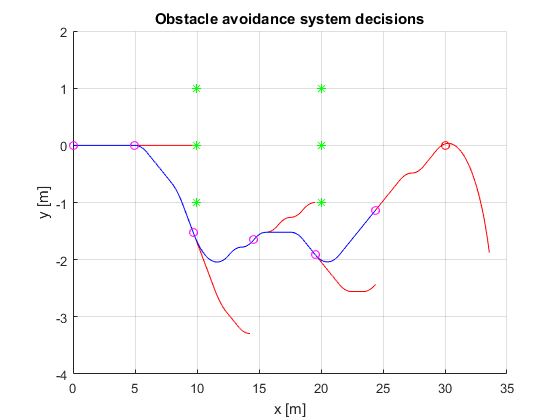
\includegraphics[width=0.7\linewidth]{\FIGDIR/70_PathPlanning_vs_Execution.png}
    \caption{Planned movements (red) vs. Executed movements (blue).}
    \label{fig:planVSExecutionSimple}
\end{figure}
\noindent Aggregated view of all planned movements $\cup B_P(i)$ (red) and all executed movements $\cup B_E(i)$ (blue) for decision frames $\mathscr{D}(t_d);t_d=\{0,5,10,15,25\}$ is portrayed in figure \ref{fig:planVSExecutionSimple}. Two collision situations were inverted in frames $\mathscr{D}(10)$ to obstacle set $\mathscr{O}_1$ and $\mathscr{D}(20)$ to obstacle set $\mathscr{O}_2$.
\begin{figure}[H]
    \centering
    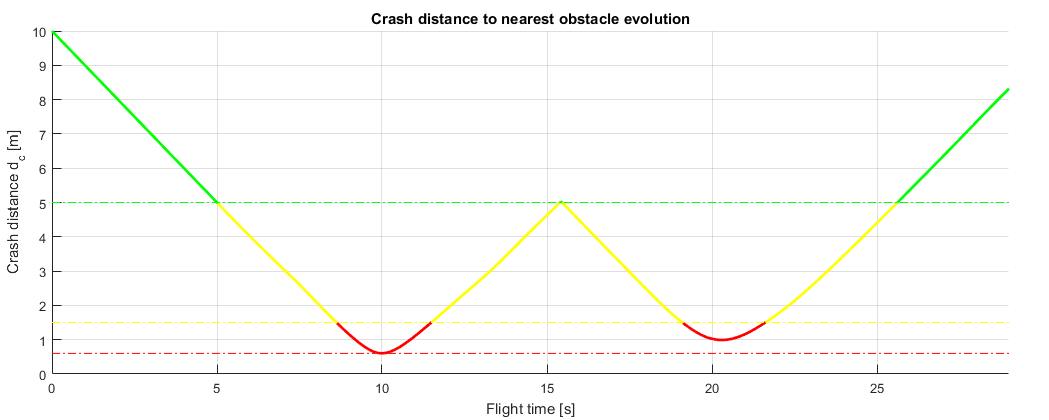
\includegraphics[width=0.8\linewidth]{\FIGDIR/61_Crash_distance_to_nearest_obstacle_evolution_known_world.png}
    \caption{Vehicle crash distance $d_c$ evolution during flight}
    \label{fig:vehicleCrashDistanceEvolutionDecisions}
\end{figure}
\noindent Crash distance $d_c$ evolution is portrayed in figure \ref{fig:vehicleCrashDistanceEvolutionDecisions}. Minimal crash distance $d_c$ never crossed safety margin $s_m$ therefore safety condition $min(d_c)\ge s_m$ is considered as satsfied. 

\subsection{Mission plan execution}
\noindent Vehicle executes mission plan defined in section \ref{ch:3DPlaygroundDefinition}. This simulation considers only notable detection frames $\mathscr{D}(t_d)$ at time of decision $t_d$. This cased shows what happens during complex mission execution.

Movement between waypoints are portrayed in figures \ref{fig:43firstwaypointMovement}, \ref{fig:45secondwaypointMovement}, \ref{fig:47thirdwaypointMovement}, \ref{fig:fourthObstacleGrid}. \textit{Red circles} represents waypoints $\mathscr{WP}$, \textit{magenta circles} represents avoidance decision points $\mathscr{D}(t_d)$, \text{blue line} represents vehicle trajectory in $\R^3$, \textit{black dashed line} represents visibility gird $\mathscr{G}_{3D}$ in time of obstacle avoidance $t_i$, \textit{green stars} represents detected obstacle points $o_i\in\mathscr{O}\subset\mathscr{G}_{3D}$.

Obstacle avoidance in given visibility grid $\mathscr{G}_{3D}$ during escape calculation are portrayed in figures \ref{fig:44ObstacleAvoidance}, \ref{fig:46ObstacleAvoidance}, \ref{fig:48ObstacleAvoidance}. \textit{Cyan dashed line} represents boundary of visibility cells $c_{i,j,k}$ in avoidance grid $\mathscr{A}(t_d)$. Each cell state is represented by point at their center, for reachable cells \textit{green cross} is used, for unreachable cells \textit{black cross} is used, for obstacle cells \textit{red circle is used}, for uncertain cells \textit{magenta circle} is used. avoidance trajectory $\mathscr{T}(x_{t_d},B)$ from reduced reach set $\mathscr{R}(t_d,t_{d+5},x_{t_d})$ is displayed as \textit{red line}.
\begin{figure}[H]
    \begin{subfigure}{0.5\textwidth}
    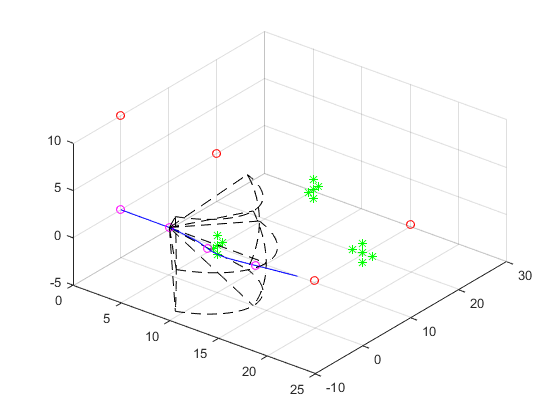
\includegraphics[width=0.9\linewidth]{\FIGDIR/43_First_waypoint_movement.png} 
    \caption{Movement to waypoint.}
    \label{fig:43firstwaypointMovement}
    \end{subfigure}
    \begin{subfigure}{0.5\textwidth}
    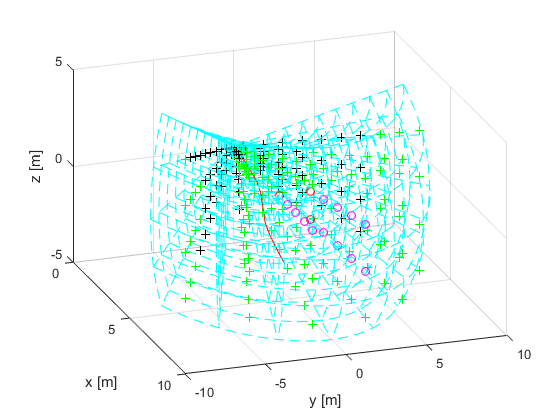
\includegraphics[width=0.9\linewidth]{\FIGDIR/44_First_osbtacle_avoidance.png}
    \caption{Avoidance grid $\mathscr{A}(t_5)$}
    \label{fig:44ObstacleAvoidance}
    \end{subfigure}
\caption{Obstacle avoidance at $\mathscr{WP}_1=[20,0,0]^T$, with best avoidance maneuver in reachable set.}
\label{fig:firstObstacleGrid}
\end{figure}
\noindent Vehicle encounters first obstacle set $\mathscr{O}_1$ at decision time $t_d=5s$. Avoidance grid $\mathscr{A}(t_5)$is initialized and filled with obstacles, reduced reach set $\mathscr{R}(t_5,t_{10},x_{5})$ is obtained. Right avoidance is executed and vehicle continues to move to goal waypoint $\mathscr{WP}_1$.
Executed movements during flight from $\mathscr{WP}_S$ to $\mathscr{WP}_1$ have follow values: $B_{\mathscr{MA}}$ = \textit{[$\circledcirc$(5), right(1), $\circledcirc$(2), $\Rightarrow$(1), $\circledcirc$(1), $\Leftarrow$(3), $\circledcirc$(6)]}
\begin{figure}[H]
    \begin{subfigure}{0.5\textwidth}
    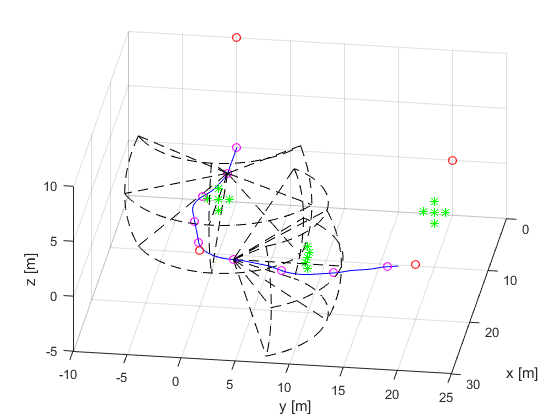
\includegraphics[width=0.9\linewidth]{\FIGDIR/45_Second_waypoint_movement.png} 
    \caption{Movement to waypoint.}
    \label{fig:45secondwaypointMovement}
    \end{subfigure}
    \begin{subfigure}{0.5\textwidth}
    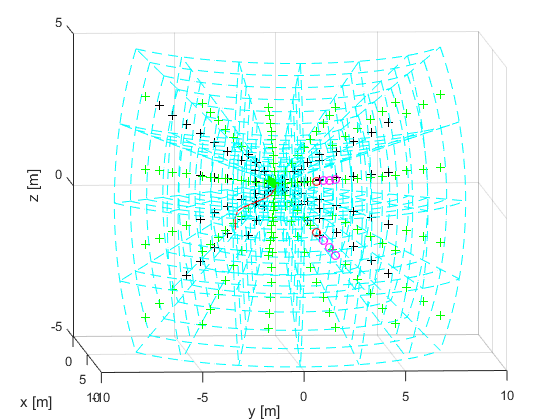
\includegraphics[width=0.9\linewidth]{\FIGDIR/46_Second_obstacle_avoidance.png}
    \caption{Avoidance grid $\mathscr{A}(t_{25}$}
    \label{fig:46ObstacleAvoidance}
    \end{subfigure}
\caption{Obstacle avoidance at $\mathscr{WP}_2=[20,20,0]^T$. with best avoidance maneuver in reachable set.}
\label{fig:secondObstacleGrid}
\end{figure}
\newpage
\noindent Vehicle reaches waypoint $\mathscr{WP}_1$ and sets waypoint $\mathscr{WP}_2$ as new goal waypoint. Vehicle executes sharp left turn. Obstacle set $\mathscr{O}_2$ is detected at time of decision $t_d=25s$. Similar maneuvers are executed as in case of obstalce set $\mathscr{O}_1$.
Executed movements buffer during flight from $\mathscr{WP}_1$ to $\mathscr{WP}_2$ have follow values: $B_{\mathscr{MA}}$ = \textit{[$\Leftarrow$(5), right(1), $\circledcirc$(2), right(1), $\circledcirc$(1), $\Leftarrow$(3), $\circledcirc$(1), $\Leftarrow$(1), right(1), $\circledcirc$(1), $\Leftarrow$(1), right(1), $\circledcirc$(1)]}.
\begin{figure}[H]
    \begin{subfigure}{0.5\textwidth}
    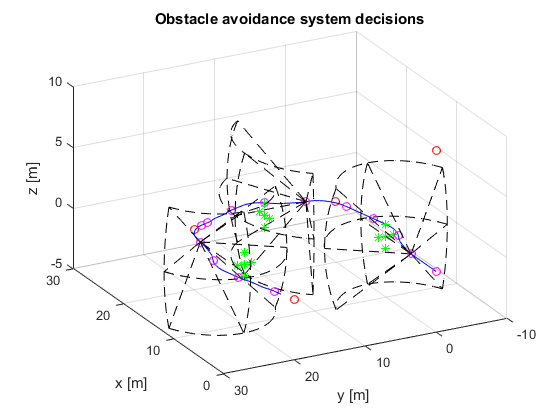
\includegraphics[width=0.9\linewidth]{\FIGDIR/47_Third_waypoint_movement.png} 
    \caption{Movement to waypoint.}
    \label{fig:47thirdwaypointMovement}
    \end{subfigure}
    \begin{subfigure}{0.5\textwidth}
    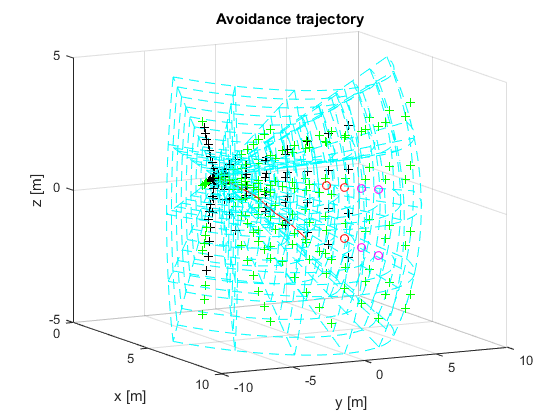
\includegraphics[width=0.9\linewidth]{\FIGDIR/48_Third_obstacle_avoidance.png}
    \caption{Avoidance grid $\mathscr{A}(t_{50})$}
    \label{fig:48ObstacleAvoidance}
    \end{subfigure}
\caption{Obstacle avoidance at $\mathscr{WP}_3=[0,20,0]^T$. with best avoidance maneuver in reachable set.}
\label{fig:thirdObstacleGrid}
\end{figure}
\noindent Vehicle reaches waypoint $\mathscr{WP}_2$ and sets waypoint $\mathscr{WP}_3$ as new goal waypoint. Vehicle executes sharp left turn. Obstacle set $\mathscr{O}_3$ is detected at time of decision $t_d=50s$. Similar maneuvers are executed as in case of obstalce set $\mathscr{O}_2$.
Executed movements during flight from $\mathscr{WP}_2$ to $\mathscr{WP}_3$ have follow values: $B_{\mathscr{MA}}$ = \textit{[$\Leftarrow$(5), right(1), $\circledcirc$(2), right(1), $\circledcirc$(1), $\Leftarrow$(3), $\circledcirc$(1), $\Leftarrow$(1), right(1), $\circledcirc$(1), $\Leftarrow$(1), right(1), $\circledcirc$(1)]}.
\begin{figure}[H]
    \centering
    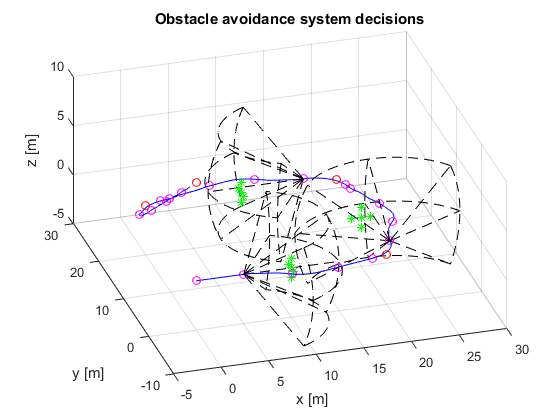
\includegraphics[width=0.6\linewidth]{\FIGDIR/49_Fourth_waypoint_movement.png}
    \caption{Optimal minimal cost flight to $\mathscr{WP}_E=[0,0,10]^T$, no avoidance have been executed.}
    \label{fig:fourthObstacleGrid}
\end{figure}
\newpage
\noindent Vehicle reaches waypoint $\mathscr{WP}_3$ and sets waypoint $\mathscr{WP}_E$ as new goal waypoint. Vehicle executes sharp left turn with increasing altitude to reach final waypoint $\mathscr{WP}_E$. 
Movement automaton buffer during flight from $\mathscr{WP}_3$ to $\mathscr{WP}_E$ have follow values: $B_{\mathscr{MA}}$ = \textit{[$\Leftarrow$(3), $\Uparrow$(1), $\Leftarrow$(2), $\Uparrow$(1), $\Leftarrow$(1), right(1), $\circledcirc$(1) ,$\Leftarrow$(1), right(1), $\Leftarrow$(1), right(1), $\circledcirc$(1), $\Leftarrow$(1), right(1), $\Leftarrow$(1), right(1), $\circledcirc$(1), $\Leftarrow$(1), right(1), $\circledcirc$(1)]}.
Simulation stops when final waypoint $\mathscr{WP}_E$ is reached.

\begin{figure}[H]
    \centering
    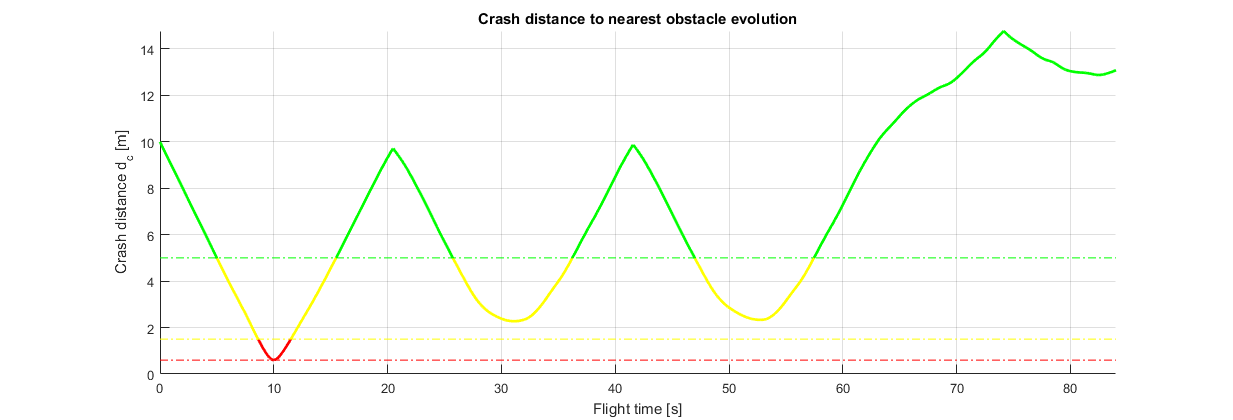
\includegraphics[width=0.95\linewidth]{\FIGDIR/59_Crash_distance_to_nearest_obstacle_evolution.png}
    \caption{Vehicle crash distance $d_c$ evolution during flight}
    \label{fig:vehicleCrashDistanceEvolution}
\end{figure}
\noindent Vehicle crash distance $d_c$ evolution during flight simulation have been measured to closest known obstacle $o_i\in\mathscr{O}$ in known world $\mathscr{F}$.  Figure \ref{fig:vehicleCrashDistanceEvolution}. shows crash distance evolution. Distance have been divined into following levels:
\begin{enumerate}
    \item \textit{Safe distance (green)} - distance where crash is avoidable, in this case $distance \ge 5 m$, this distance is threshold for conservative methods. 
    \item \textit{Cautious distance (yellow)} - distance where crash is avoidable with additional effort using special maneuver, in this case $1.5m \ge distance < 5m$, this distance is best performance for methods with obstacle classification.
    \item \textit{Dangerous distance (red)} - distance where crash is invertible in case of noncolinear obstacle heading, in this case $0.6m \ge distance < 1.5m$, this distance can be only performed by presented obstacle avoidance algorithm.
\end{enumerate}
\noindent During simulation only closest distance to obstacle of 0.7 meter have been reached. This proves that presented avoidance algorithm keeps given safety margin $s_m=0.6 m$ also in practical implementation. The theoretical obstacle distance is best in state of art of theoretical avoidance systems.

Prediction quality is very important factor in predictive control, therefore quantitative measurement for prediction of this system have been introduced (\ref{eq:movementAutomatonPredictionError2}). Movement automaton prediction error $e_p$ is based on mean square prediction error (MSE).
\begin{equation}\label{eq:movementAutomatonPredictionError2}
    e_p=\sqrt{\sum_{t_i=t_0+i}^{i\in\{1,\dots,n\}} \left (\hat{x}(t_i)-x(t_i)\right)^2}    
\end{equation}

\noindent Movement automaton prediction error compares predicted state $\hat{x}$ and real system state $x$ for each movement execution time $t_i$. Movement execution time in this case was $s_1$ so time $t_i$ was defined as $t_i=t_0+i, i\in\{1,\dots,n\}$, where n is total count of executed movements. Movement automaton prediction error $e_p$ was in this case $e_p\approx 0$.
\begin{figure}[H]
    \centering
    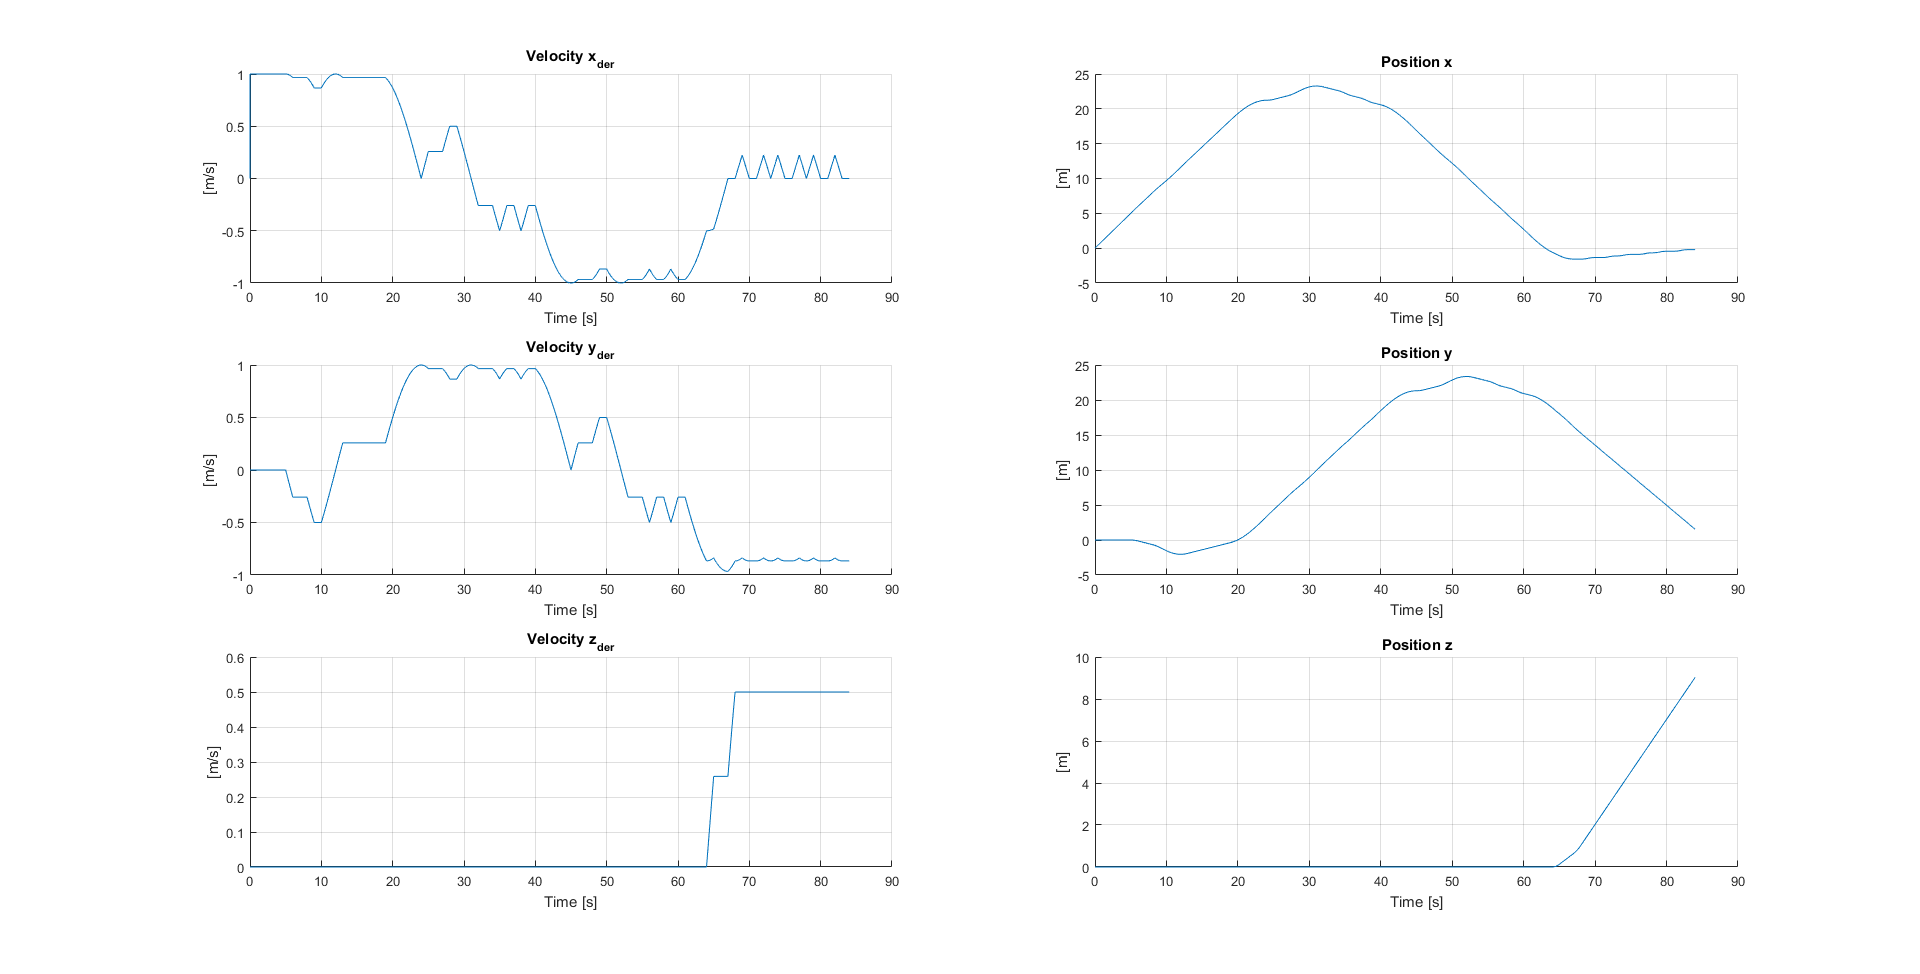
\includegraphics[width=\linewidth]{\FIGDIR/50_Vehicle_position.png}
    \caption{Vehicle position $x,y,z$ and their derivations $\dot{x},\dot{y},\dot{z}$ evolution during flight.}
    \label{fig:vehicleStateGrid1}
\end{figure}
\noindent Vehicle position $x,y,z$ and their derivations $\dot{x},\dot{y},\dot{z}$ and their evolution during flight is portrayed in figure \ref{fig:vehicleStateGrid1}. Brown color is used for predicted model state and blue color is used for real model parameter evolution. Both models are equal, supported by movement automaton prediction error $e_p\approx 0$.
\begin{figure}[H]
    \centering
    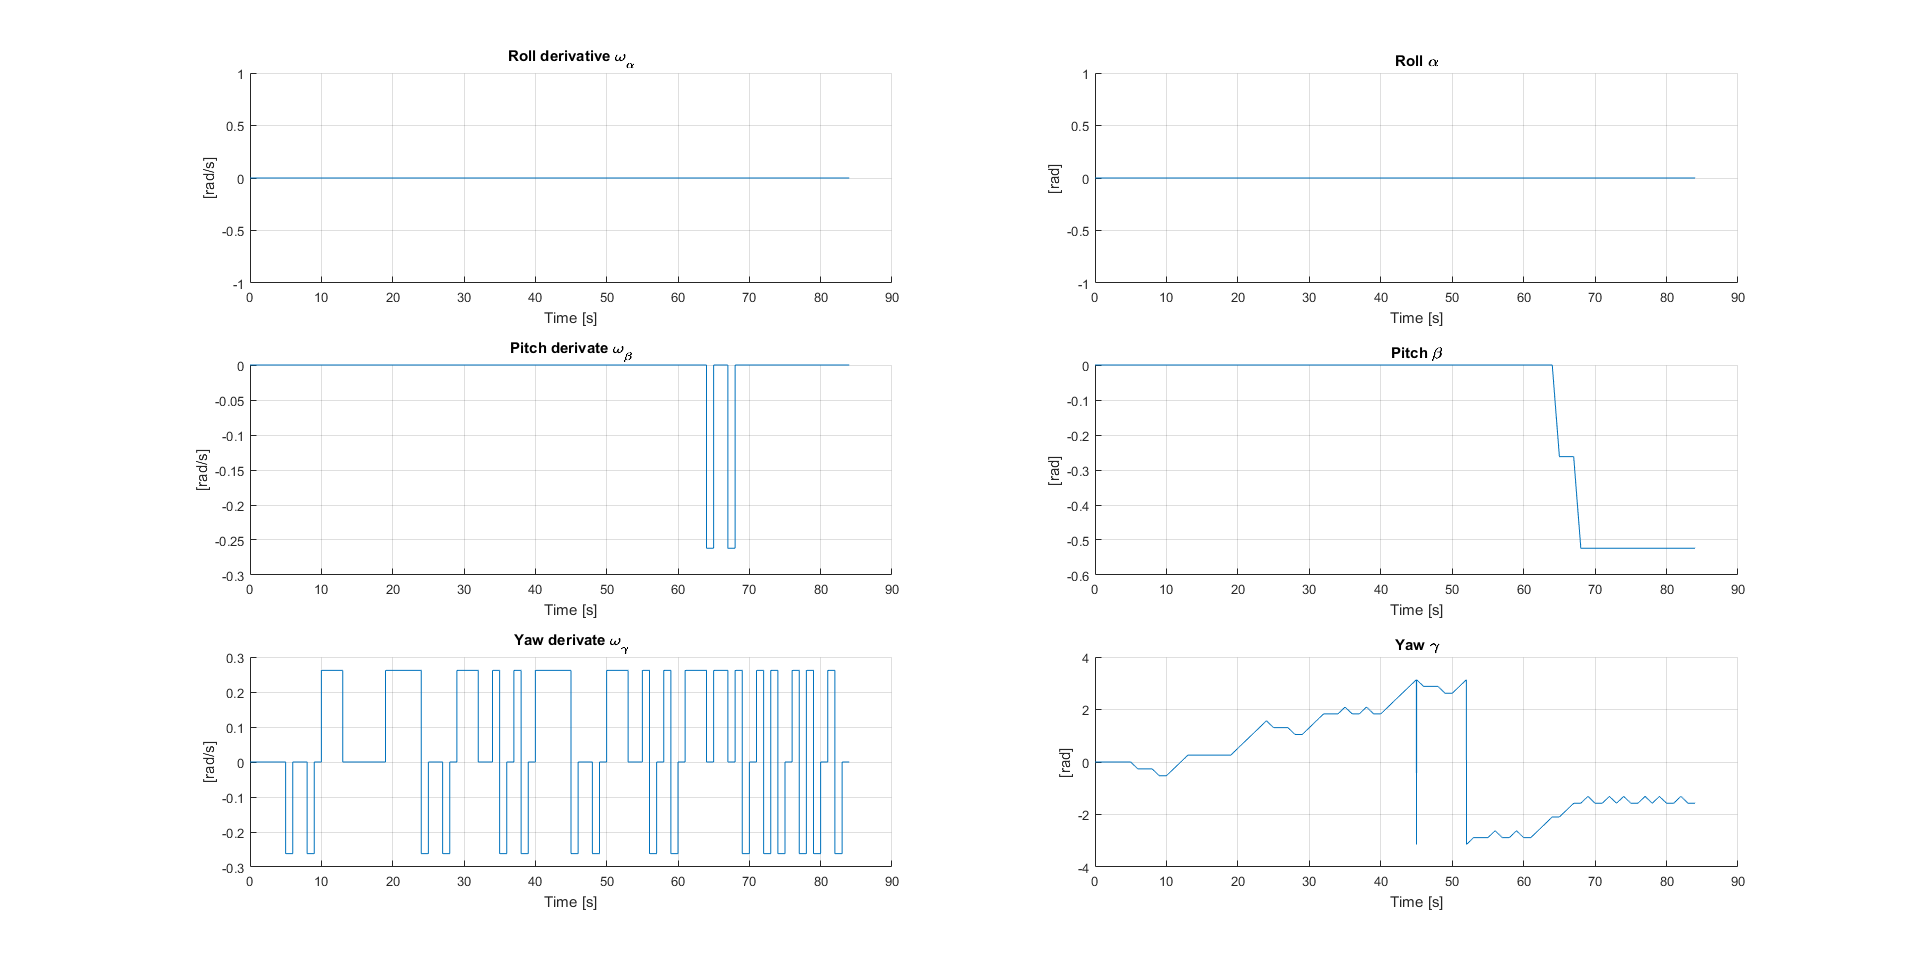
\includegraphics[width=\linewidth]{\FIGDIR/51_Vehicle_angles.png}
    \caption{Vehicle positional angles $\alpha,\beta,\gamma$ and their angular velocities $\omega_\alpha,\omega_\beta,\omega_\gamma$ evolution during flight}
    \label{fig:vehicleStateGrid2}
\end{figure}
\noindent Similar to previous comparison (fig. \ref{fig:vehicleStateGrid1}.) Comparison for vehicle positional angles $\alpha,\beta,\gamma$ and their angular velocities $\omega_\alpha,\omega_\beta,\omega_\gamma$ evolution during flight holds previous assumption (fig. \ref{fig:vehicleStateGrid2}).
\bibliography{thesis}
\chapter*{Annex}\noindent
\noindent This chapter contains required linear algebra supplements used in this work for estimation, projection and rotation in euclidean space. 

3-dimensional Cartesian space gives us an x, y, and z axis (describing position based on horizontal placement, vertical placement, and depth respectively). The coordinates for any point within this space are shown as a tuple $(x,y,z)$. Coordinate system used this work will be viewed as right-handed system (thumbs points at positive direction of x-axis, index finger is pointing to positive direction of y-axis, then positive  direction of z axis is shown by remaining fingers).

Euler have worked on universal rotation theorem which was presented in \cite{euler1775formulae}. Rigid body dynamics and rotation matrices have been proposed in book by Schaub \cite{schaub2003analytical}. Local coordinates are used, where plane center of gravity is used as center point and plane heading is oriented to X axis. This local coordinate system is called Euler Normalized Unit-frame (ENU). Rotation matrices are used to transform between two displaced coordinate systems. Roll angle $\alpha$ rotation is defined around X-axis by matrix (\ref{eq:rollTransformationMatrix}) on YZ-plane. Pitch angle $\beta$ rotation matrix is defined around Y-axis by matrix (\ref{eq:pitchTransformationMatrix}) on XZ plane. Yaw angle $\gamma$ rotation matrix is defined around Z axis by matrix (\ref{eq:yawTranformationMatrix}) on XY plane.

\begin{equation}\label{eq:rollTransformationMatrix}
    R_{YZ} = R_\alpha =
    \begin{bmatrix}
        1 & 0 & 0\\
        0 & \cos(\alpha) & -\sin(\alpha)\\
        0 & \sin(\alpha) & \cos(\alpha)
    \end{bmatrix}
\end{equation}
\begin{equation}\label{eq:pitchTransformationMatrix}
    R_{XZ} = R_\beta =
    \begin{bmatrix}
        \cos(\beta) & 0 & \sin(\beta)\\
        0 & 1 & 0\\
        -\sin(\beta) & 0 & \cos(\beta)
    \end{bmatrix}
\end{equation}
\begin{equation}\label{eq:yawTranformationMatrix}
    R_{XY} = R_\gamma = 
    \begin{bmatrix}
        \cos(\gamma) & -\sin(\gamma) & 0 \\
        \sin(\gamma) & \cos(\gamma) & 1 \\
        0 & 0 & 1
    \end{bmatrix}
\end{equation}
Final rotation matrix in XYZ ordered space is given by equation(\ref{eq:xyzspaceRotationMatrix}).
\begin{equation}\label{eq:xyzspaceRotationMatrix}
    \begin{aligned}
        R_{XYZ}  =& R_{\alpha\beta\gamma} =  R_{XY} * R_{XZ} * R_{YZ} = R_\gamma * R_\beta *R_\alpha\\
         =& 
         \small
         \begin{bmatrix}
            \cos\beta\cos\gamma & \cos\gamma\sin\alpha\sin\beta - \cos\alpha\sin\gamma & \sin\alpha\sin\gamma + \cos\alpha\cos\gamma\sin\beta \\
            \cos\beta\sin\gamma & \cos\alpha\cos\gamma + \sin\alpha\sin\beta\sin\gamma & \cos\alpha\sin\beta\sin\gamma - \cos\gamma\sin\alpha \\
            -\sin\beta & \cos\beta\sin\alpha & \cos\alpha\cos\beta 
         \end{bmatrix}
         \normalsize
    \end{aligned}
\end{equation}
To keep solution numerically stable and rotations numerically stable gimbal lock prevention is necessary \cite{kramer1977gyro}. Gimbal lock occurs when one of matrices (\ref{eq:rollTransformationMatrix}, \ref{eq:pitchTransformationMatrix}, \ref{eq:yawTranformationMatrix}) is singular or final matrix for XYZ rotation is singular (\ref{eq:xyzspaceRotationMatrix}). Gimbal lock leads to loose of one or more degree of freedom, depending on rank and space dimension of singular matrix. To prevent gimbal lock it is necessary to introduce mechanism to check if rotation matrix is regular. For this purpose normative reset function is introduced:
\begin{equation}
    \left [ \alpha, \beta ,\gamma \right ]^T = f(t,\alpha^-,\beta^-,\gamma^-), \quad \textnormal{norm}(R_{\alpha\beta\gamma})=3
\end{equation}
Function resets yaw $\gamma$ or roll $\alpha$ angle to initial position to keep degree of rotation matrix. Simpler but not fault tolerant solution is to keep angles $\alpha,\beta,\gamma, \in \left (  -\pi,\pi\right ]$ range.

\subsection*{Transformation between coordinate systems}
\noindent Polar coordinate system represents point in form of vector $[distance$, $angle_{horizontal}$, $angle_{vertical}]$, which is ideal for representation of LiDAR scanned point, because usually total point distance andpair of angles are returned. Using most common LiDAR with horizontal rotation $\theta$ and vertical mirror inclination $\varphi$, one can define planar coordinate $p_{planar} = [d_{xyz},\theta,\varphi]$ which is dual to Cartesian coordinate $p_{cartesian} = [x,y,z]$. If rotation angles are forced to stay as $\theta,\varphi\in(-\pi,\pi]$ transformation function is bijection.

Transformation from planar to Cartesian representation is defined by following series of functions (\ref{eq:cpt01}, \ref{eq:cpt02},\ref{eq:cpt03}, \ref{eq:cpt04}).
\begin{equation}\label{eq:cpt01}
    d_{xy} = \cos\varphi.d_{xyz}
\end{equation}
\begin{equation}\label{eq:cpt02}
    z = \sin\varphi.d_{xyz}
\end{equation}
\begin{equation}\label{eq:cpt03}
    y = \sin\theta.d_{xy}
\end{equation}
\begin{equation}\label{eq:cpt04}
    x = \cos\theta.d_{xy}
\end{equation}
Transformation from Cartesian to planar representation is defined by following series of functions (\ref{eq:cpt05}, \ref{eq:cpt06},\ref{eq:cpt07}, \ref{eq:cpt08}).
\begin{equation}\label{eq:cpt05}
    d_{xyz} = \sqrt{x^2+y^2+z^2}    
\end{equation}
\begin{equation}\label{eq:cpt06}
    d_{xy} = \sqrt{x^2+y^2}    
\end{equation}
\begin{equation}\label{eq:cpt07}
    \theta = \arctan\frac{y}{x}
\end{equation}
\begin{equation}\label{eq:cpt08}
    \varphi= \arctan\frac{z}{d_{xy}}
\end{equation}

\begin{definition}{Global coordinate system $\mathscr{X}_\mathscr{G}$}\label{def:globalCoordinateSystem}
    takes as center $c_{\mathscr{G}0}$ well known point (for example center of geo-reference model in GNSS systems) every reference distance, plane or angle is calculated taking this center to mind.
\end{definition}
\begin{definition}{Local coordinate system $\mathscr{X}_\mathscr{L}$}\label{def:localCoordinateSystem}
    takes as center $c_{\mathscr{L}0}$ frame of vehicle and can be changing position and orientation in global coordinate frame $\mathscr{X}_\mathscr{G}$.
\end{definition}
\begin{definition}{Global position of planar obstacle $o_i\in\mathscr{O}_{3D}$.}\label{def:globalObstaclePosition3D}
    Let $o_i = [d_o, \theta_o, \varphi_o]^T$ be planar position of obstacle $o_i$ in local coordinate frame of vehicle with global Cartesian position $[x,_v,y_v,z_v]^T$ and normalized orientation angles $[\alpha_v,\beta_v,\gamma_v]$.\\
    Then Cartesian position of obstacle $oi$, $[x_o,y_o,z_o]^T$  in local coordinate frame is given by transformation functions $x_o$ (\ref{eq:cpt04}), $y_o$ (\ref{eq:cpt03}), $z_o$ (\ref{eq:cpt02}).\\ 
    Global  position of planar obstacle $oi$, $[x_g,y_g,z_g]^T$ is given by following equation:
    \begin{equation}
        \begin{bmatrix}
            x_g\\y_g\\z_g
        \end{bmatrix}
        =
        \left [
            R_{XYZ}(\alpha_v,\beta_v,\gamma_v)
            \begin{bmatrix}
                x_o\\y_o\\z_o
            \end{bmatrix}
            +
            \begin{bmatrix}
                x_v\\y_v\\z_v
            \end{bmatrix}
        \right ]
    \end{equation}    
\end{definition}
\newpage
\begin{definition}{Local position of global coordinate $[x_g,y_g,z_g]^T\in\R^3$.}\label{def:globalToLocal}
    Let there be vehicle with global Cartesian position $[x,_v,y_v,z_v]^T$ and normalized orientation angles $[\alpha_v,\beta_v,\gamma_v]$. in global coordinate frame $\mathscr{X}_\mathscr{X}$.\\
    Then local Cartesian coordinate position $[x_l,y_l,z_l]^T$ of point $[x_g,y_g,z_g]^T$ is given by following equation:
    \begin{equation}
        \begin{bmatrix}
            x_l\\y_l\\z_l
        \end{bmatrix}
        =
        \left [
            R_{XYZ}(-\alpha_v,-\beta_v,-\gamma_v)
            \left (
            \begin{bmatrix}
                x_g\\y_g\\z_g
            \end{bmatrix}
            -
            \begin{bmatrix}
                x_v\\y_v\\z_v
            \end{bmatrix}
            \right )
        \right ]
    \end{equation}
    Local planar position is given as $[d_l, \theta_l,\varphi_l]$, where $d_l$ is given by (\ref{eq:cpt05}), $\theta_l$ is givent by (\ref{eq:cpt07}). $\varphi_l$ is given by (\ref{eq:cpt08}), where $[x_l,y_l,z_l]$ are used as local coordinates.
\end{definition}
\end{document}
